\documentclass[a4paper,12pt]{article}

% For content
\usepackage[nottoc,numbib,notlof,notlot]{tocbibind}

% No intetation
\usepackage[parfill]{parskip}

% Multirow tables
\usepackage{multirow}

% Calligraphic math
% \usepackage{calrsfs}
% \usepackage{boondox-cal}

% Paragraph new line
\newcommand{\paragraphLine}[1]{\paragraph{#1}\mbox{}\\}

\usepackage{amsmath}
\DeclareMathOperator*{\argmin}{\arg\!\min}
\newcommand{\argminUnder}{\arg\!\min}
\newcommand{\argminB}{\mathop{\mathrm{argmin}}}
\usepackage{mathtools}
\DeclarePairedDelimiter\abs{\lvert}{\rvert}
% \DeclarePairedDelimiter\norm{\lVert}{\rVert}
\newcommand\norm[1]{\left\lVert#1\right\rVert}

% R symbol
\usepackage{amssymb}
\newcommand{\R}{\mathbb{R}}

% For bold
\usepackage{bm}

% Font
\usepackage{fontspec}
\setmainfont{GFS Artemisia}

% English-Greek use
\usepackage{polyglossia}
% \setmainlanguage{english}
% \setotherlanguage{greek}
\setmainlanguage{greek}
\setotherlanguage{english}

\iffalse
\usepackage[greek, english]{babel}
\fi

\newfontfamily\greekfont{GFS Artemisia}
\let\greekfonttt\ttfamily

% Hyperlinks
\usepackage[hidelinks, pdfencoding=auto]{hyperref}
\renewcommand{\figureautorefname}{Σχήμα}
\renewcommand{\tableautorefname}{Πίνακας}

% Images
\usepackage{graphicx}
\graphicspath{{./images/}}
\usepackage[font={footnotesize,it}]{caption}
\usepackage[font={footnotesize}]{subcaption}
\renewcommand{\thesubfigure}{\Roman{subfigure}}
\usepackage{float}

% New page every section
\usepackage{titlesec}
\newcommand{\sectionbreak}{\clearpage}

% References
\usepackage[backend=biber,style=ieee]{biblatex}
\addbibresource{references.bib}
% \bibliography{references} 

\usepackage[justify]{ragged2e}
% \justifying

% Defines a new command for the horizontal lines, change thickness here
\newcommand{\HRule}{\rule{\linewidth}{0.5mm}}

\tolerance=10000 
% \pretolerance=10000

\begin{document}

\begin{titlepage}

\center
 
\textsc{\LARGE Αριστοτέλειο Πανεπιστήμιο Θεσσαλονίκης}

% \vspace{1cm}


\includegraphics[scale=.3]{LogoAUTH72ppi.png}

% \vspace{1cm}
\textsc{\Large Τμήμα Ηλεκτρολόγων Μηχανικών και Μηχανικών Υπολογιστών}
\vspace{0.5cm}

\textsc{\large Τομέας Ηλεκτρονικής και Υπολογιστών}
\vspace{0.5cm}

\HRule
\vspace{0.4cm}
{ \huge \bfseries Τίτλος διπλωματικής}
\vspace{0.4cm}
\HRule
\vspace{1cm}

\begin{minipage}{0.8\textwidth}
    \center
    \large
    \emph{Συγγραφέας:} \\ 
    \Large
    Κωστινούδης Ευάγγελος
\end{minipage}
\vspace{0.5cm}

\begin{minipage}{0.8\textwidth}
    \center
    \large
    \emph{Επιβλέπων καθηγητής:} \\ 
    \Large
    Θεοχάρης Ιωάννης \\
\end{minipage}
\vspace{0.5cm}

\begin{minipage}{0.8\textwidth}
    \center
    \large
    \emph{Επιβλέπων Υποψήφιος Διδάκτορας:} \\ 
    \Large
    Χαδουλός Χρήστος
\end{minipage}
\vspace{0.5cm}

\vspace*{\fill}

% {\large \today}
{\large Απρίλιος, 2021}

\end{titlepage}

\begin{titlepage}

\begin{center}
    \HRule
    \vspace{0.4cm}
    { \huge \bfseries Thesis Title in english}
    \vspace{0.4cm}
    \HRule
    \vspace{1.5cm}

    \begin{minipage}{0.8\textwidth}
    \center
    \large
    \emph{Author:} \\ 
    \Large
    Kostinoudis Evangelos
    \end{minipage}
    \vspace{0.5cm}

    \begin{minipage}{0.8\textwidth}
        \center
        \large
        \emph{Supervisor professor:} \\ 
        \Large
        Theocharis Ioannis
    \end{minipage}
    \vspace{0.5cm}

    \begin{minipage}{0.8\textwidth}
        \center
        \large
        \emph{Supervisor PhD Student:} \\ 
        \Large
        Chadoulos Christos
    \end{minipage}
    \vspace{0.5cm}
\end{center}
\end{titlepage}

\section*{Ευχαριστίες}

Σε αυτό το σημείο θα ήθελα να ευχαριστήσω θερμά τον καθηγητή Θεοχάρη Ιωάννη και
τον υποψήφιο διδάκτορα Χαδουλό Χρήστο για την καθοδήγηση, την βοήθεια και τις
συμβουλές τους για την εκπόνηση της διπλωματικής εργασίας.


\section*{Περίληψη}

Οι εξελίξεις στη μηχανική μάθηση και συγκεκριμένα στην κατάτμηση εικόνων
μέσω αυτής επιτρέπουν να λυθεί αυτόματα το πρόβλημα της κατάτμησης ιατρικών
απεικονίσεων, το οποίο είναι χρονοβόρο και μπορεί να υλοποιηθεί μόνο από
ειδικούς. Στην παρούσα διπλωματική εργασία, παρουσιάζονται τρεις μέθοδοι
μηχανικής μάθησης κατάτμησης ιατρικών απεικονίσεων και συγκεκριμένα απεικονίσεων
μαγνητικής τομογραφίας γονάτων. Οι ανατομικές δομές που χρησιμοποιήθηκαν είναι
τα οστά και οι χόνδροι. Τα δεδομένα που χρησιμοποιήθηκαν τόσο για την εκπαίδευση
όσο για την αξιολόγηση των προτεινόμενων μεθόδων προέρχονται από το
Osteoarthritis Initiative Zuse Institute Berlin. Το αποτέλεσμα των μεθόδων
(συντελεστής ομοιότητας Dice) για ετικέτα των χόνδρων κυμαινόταν μεταξύ
0.82-0.85 και για την ετικέτα των οστών γύρο στο 0.96. 

\section*{Abstract}

Recent developments in machine learning and in particular in image segmentation
using machine learning allows the problem of medical image registration, which
is time consuming and only implemented by experts, to be solved. In this diploma
thesis, three medical image segmentaion methods are presented using machine
learing and in particular magnetic resonance imaging images of knees. The
anatomical structures used are bones and cartilage. The data used for both
training and evaluation of the proposed methods come from the Osteoarthritis
Initiative Zuse Institute Berlin. The result of the methods (Dice similarity
coefficient) for the cartilage label ranged between 0.82-0.85 and for the bone
label around at 0.96. 

\tableofcontents

\listoffigures

\listoftables

\section{Εισαγωγή}

\subsection{Διατύπωση του προβλήματος}

Η κατάτμηση είναι η διαδικασία διαμέρισης μίας εικόνας σε διάφορα ουσιαστικά
τμήματα. Σκοπός της κατάτμησης είναι η απλοποίηση ή/και η αλλαγή της
αναπαράστασης της εικόνας σε κάτι που είναι πιο σημασιολογικά σημαντικό και
είναι πιο εύκολο να αναλυθεί. Πιο συγκεκριμένα, η κατάτμηση εικόνας είναι η
διαδικασία ανάθεσης μίας ετικέτας σε κάθε εικονοστοιχείο της εικόνας έτσι ώστε
τα εικονοστοιχεία με την ίδια ετικέτα να έχουν ίδια χαρακτηριστικά.

Στην ιατρική απεικόνιση αυτά τα τμήματα αντιστοιχούν συχνά σε διαφορετικές
κατηγορίες ιστών, οργάνων, παθολογίες ή άλλες βιολογικά σχετιζόμενες δομές. Η
αυτοματοποιημένη κατάτμηση ιατρικών απεικονίσεων μπορεί να βοηθήσει τους
γιατρούς επιταχύνοντας τη διαδικασία διάγνωσης. Η καθημερινή δημιουργία πληθώρας
ιατρικών απεικονίσεων καθιστά τη χειροκίνητη κατάτμηση από ειδικούς όλο και
δυσκολότερη, λόγο του χρονικού διαστήματος που χρειάζεται η ανάλυση. Επομένως, η
ανάπτυξη αξιόπιστων, σταθερών και ακριβών τεχνικών για την αυτοματοποιημένη
κατάτμηση ιατρικών απεικονίσεων αποτελεί μία σημαντική πρόκληση.

\subsubsection{Κατάτμηση βάση ατλάντων}

Η κατάτμηση απεικονίσεων βάση ατλάντων αποτελεί την διαδικασία κατά την οποία
χρησιμοποιούνται απεικονίσεις που έχουν κατανεμηθεί από κάποιον ειδικό, ούτως
ώστε να επιτευχθεί η κατάτμηση της νέας απεικόνισης. Οι μέθοδοι αυτοί συνήθως
απαιτούν την χρήση καταχώρησης εικόνας (image registration) με σκοπό την
ευθυγράμμιση τού ή των ατλάντων στην εικόνα-απεικόνιση που πρόκειται να
κατανεμηθεί \cite{Registration_Segmentation:1}.

\subsubsection{Αντικείμενο διπλωματικής εργασίας}

Στην διπλωματική εργασία εφαρμόστηκαν μέθοδοι κατάτμησης ιατρικών απεικονίσεων
βάση ατλάντων με χρήση μηχανικής μάθησης \cite{Zhang:1} \cite{Tong:1}
\cite{Coupe:1}. Οι απεικονίσεις αφορούν μαγνητικές τομογραφίες σε γόνατα και οι
περιοχές κατάτμησης αποτελούνται από τους αρθρικούς χόνδρους και τα οστά. Τα
δεδομένα που χρησιμοποιήθηκαν προέρχονται από το Osteoarthritis Initiative Zuse
Institute Berlin (OAI ZIB). Οι μέθοδοι που χρησιμοποιήθηκαν προέρχονται από
μεθόδους που έχουν χρησιμοποιηθεί για την κατάτμηση περιοχών του εγκεφάλου.
% TODO: references


\section{Θεωρητικό υπόβαθρο}

\subsection{Πλαίσιο συγχώνευσης κατηγοριών βασισμένο σε γράφους}
\label{Graph-Based_Framework:1}

Το πλαίσιο συγχώνευσης κατηγοριών βασισμένο σε γράφους προτάθηκε από
το \cite{Zhang:1} ως μία μέθοδος μέσω της οποίας μπορούν να παραχθούν πολλές
υπάρχουσες μέθοδοι συγχώνευσης κατηγοριών.

Έστω το ζεύγος $\{(I_i,L_i),i=1,...,n\}$ όπου $I_i$ είναι η απεικόνιση ενός
άτλαντα, $L_i$ ο χάρτης των κατηγοριών της αντίστοιχης απεικόνισης και $n$ το
σύνολο των ατλάντων. Δοθείσας μία απεικόνισης $I$, δημιουργείται ο σταθμισμένος
γράφος $G_i$ μεταξύ των εικονοστοιχείων $\bm{x}$ της δοθείσας εικόνας $I$ και
του εικονοστοιχείου $\bm{y}$ της απεικόνισης του άτλαντα $I_i$, μαζί με τα
αντίστοιχα βάρη $w_i(\bm{x},\bm{y})$, για $(\bm{x},\bm{y})\in\Omega^2$, όπου
$\Omega$ ο χώρος των απεικονίσεων. Με τη δημιουργία των βαρών του γράφου, η
συγχώνευση των κατηγοριών γίνεται για κάθε $\bm{x}$ της απεικόνισης εισόδου $I$
σύμφωνα με το τύπο:

\begin{equation} \label{label_fusion:1}
    L(\bm{x})=\frac{ \sum_{i=1}^{n}  \sum_{\bm{y}\in\Omega}
                     w_i(\bm{x},\bm{y})L_i(\bm{y})}
    { \sum_{i=1}^{n}  \sum_{\bm{y}\in\Omega} w_i(\bm{x},\bm{y}) }
    , \forall \bm{x}\in\Omega
\end{equation}

$L$ είναι ο χάρτης των κατηγοριών της απεικόνισης εισόδου $I$.

% Lasso
\subsection{Ελάχιστα απόλυτος τελεστής συρρίκνωσης και επιλογή} \label{lasso:1}

Ο ελάχιστα απόλυτος τελεστής συρρίκνωσης και επιλογής (Least Absolute Shrinkage
and Selection Operator, Lasso) \cite{Lasso:1} είναι μία μέθοδος παλινδρόμησης.
Παλινδρόμηση είναι η μέθοδος πρόβλεψης της συμπεριφοράς μίας μεταβλητής
βασισμένη σε μία ή περισσότερες άλλες μεταβλητές. Έστω οι παρατηρήσεις
$(\bm{x_i},y_i), i=1,...,N$, όπου $\bm{x_i}=(x_{i1},...,x_{ip})$ οι $p$
μεταβλητές εισόδου και $y_i$ η μεταβλητή εισόδου για την $i$-οστή παρατήρηση. Αν
$\hat{\beta} = (\hat{{\beta}_1},...,\hat{{\beta}_p})^T$ και $\hat{\alpha}$ τα
αποτέλεσματα της παλινδρόμησης (συντελεστές παλινδρόμησης) τότε ο τελεστής
ορίζεται ως:

\begin{equation}\label{lassoEq1}
    (\hat{\alpha}, \hat{\beta}) = 
    \argmin{\left\{\sum_{i=1}^{N} {\left(\,y_i-\alpha- \sum_{j=1}^{p}
    \beta_{j}x_{ij}\right)}^2 \right\}} 
    \text{ subject to }
    \sum_{j=1}^{p} \abs{\beta_j} \leq t
\end{equation}

Το $t \geq 0$ είναι παράμετρος συντονισμού. Για κάθε τιμή του $t$ η λύση για το
$\alpha$ είναι $\hat{\alpha}=\overline{y}$ (όπου $\overline{y}$ είναι η μέση
τιμή του $y$). Επίσης μπορούμε να υποθέσουμε χωρίς την απώλεια της γενίκευσης
ότι $\hat{\alpha}=0$ ώστε να εξαλειφθεί το $\alpha$. Έστω $\bm{X} =
(\bm{x_1},...,\bm{x_N})^T$ και $y = (y_1,...,y_N)^T$ τότε η \eqref{lassoEq1}
μπορεί να γραφτεί ως:

\begin{equation}\label{lassoEq2}
    \hat{\beta} = 
    \argmin{\left\{\frac{1}{N} \norm{\left(\,y - \bm{X} \beta\right)}_2^2
    \right\}} 
    \text{ subject to }
    \norm{\beta}_1 \leq t
\end{equation}

Όπου η $p$-οστή νόρμα του $x=(x_1,...,x_n)$ ορίζεται ως:

\begin{equation*}
    \norm{x}_p=\left( \sum_{i=1}^{n} \abs{x_i}^p\right)^{1/p}
\end{equation*}

Η εξίσωση \eqref{lassoEq2} μπορεί να γραφτεί επίσης με την χρήση του
πολλαπλασιαστή Lagrange ως:

\iffalse
Όπου $\norm{x}_p=\left( \sum_{i=1}^{n} \abs{x_i}^p\right)^{1/p}$ είναι η
$p$-οστή νόρμα του $x=(x_1,...,x_n)$. Η εξίσωση μπορεί να γραφτεί επίσης με την
χρήση του πολλαπλασιαστή Lagrange ως:
\fi

\begin{equation}\label{lassoEq3}
    \hat{\beta} = 
    \argmin{\left\{\frac{1}{N} \norm{\left(\,y - \bm{X} \beta\right)}_2^2 +
    \lambda \norm{\beta}_1 \right\}} 
\end{equation}

Πολλές φορές οι στήλες του $\bm{X}$ κανονικοποιούνται, δηλαδή ισχύει:

\begin{equation*}
    \sum_{j=1}^{p} {\frac{x_{ij}}{N}} = 0
    \text{ , }
    \sum_{j=1}^{p} {\frac{x_{ij}^2}{N}} = 1
\end{equation*}


\iffalse
% TODO: Ίσως να το ϐαλω αυτό:
Το πλεονέκτημα του ελάχιστα απόλυτου τελεστή συρρίκνωσης και επιλογής είναι ότι
σε σχέση 
\fi

% registration
\subsection{Καταχώρηση εικόνας} \label{registration:1}

Καταχώρηση εικόνας (image registration) είναι η διαδικασία μετασχηματισμού
διαφορετικών δεδομένων σε ένα σύστημα συντεταγμένων. Η διαδικασία αυτή επιδιώκει
μέσω του μετασχηματισμού αυτού, την επικάλυψη των κοινών χαρακτηριστικών των
δεδομένων. Τα δεδομένα μπορεί να είναι πολλαπλές φωτογραφίες, δεδομένα από
διαφορετικούς αισθητήρες, ώρες, βάθη και οπτικές \cite{Registration:1}. Στις
ιατρικές απεικονίσεις επιδιώκεται μέσω του μετασχηματισμού, αντίστοιχα
εικονοστοιχεία των απεικονίσεων να αναπαριστούν όμοια βιολογικά σημεία.

Συνήθως στις μεθόδους καταχώρησης εικόνας η μία εικόνα παραμένει σταθερή κατά
την διαδικασία της καταχώρησης και η άλλη-άλλες μετασχηματίζονται. Η εικόνα που
παραμένει σταθερή αποκαλείται εικόνα αναφοράς ή απλά σταθερή εικόνα. Οι εικόνες
που μετασχηματίζονται ονομάζονται εικόνες καταχώρισης ή κινούμενες εικόνες.

%TODO: εικόνα εδώ;

Η βασική διαδικασία της καταχώρησης εικόνας αποτελείται από την ανίχνευση
χαρακτηριστικών, την ευθυγράμμιση χαρακτηριστικών από την κινούμενη εικόνα στην
σταθερή, εκτίμηση παραμέτρων συναρτήσεων χαρτογράφησης, την δειγματοληψία και
τον μετασχηματισμό εικόνας. Οι μέθοδοι καταχώρισης εικόνας είναι μοναδικές για
κάθε πρόβλημα και δεν υπάρχει κοινή τεχνική καταχώρισης εικόνας που να είναι
ισάξια αποτελεσματική σε κάθε πρόβλημα που εφαρμόζεται \cite{Registration:2}.
Για παράδειγμα υπάρχουν μέθοδοι που βασίζονται στην ένταση των εικόνων και
μέθοδοι που βασίζονται σε χαρακτηριστικά τους.

% Οι μέθοδοι της καταχώρησης εικόνας διαφέρουν ανάλογα με το δεδομένα που
% πρόκειται να καταχωρηθούν \cite{Registration:2}. 

\subsubsection{Μέση διαφορά τετραγώνων} \label{MSSD}

Στην οικογένεια των μεθόδων που βασίζονται στην ένταση των εικόνων, η μέτρηση
της ομοιότητας μεταξύ της κινούμενης και της σταθερής εικόνας αποτελεί ένα
δομικό στοιχείο της καταχώρησης εικόνας. Η μέτρηση αυτή αξιολογεί την
καταλληλότητα του μετασχηματισμού και χρησιμοποιείται για να υπολογιστεί η
παράγωγος της αξιολόγησης, ούτως ώστε να χρησιμοποιηθούν από τον αλγόριθμο
βελτιστοποίησης. Η επιλογή της μετρικής βασίζεται στο εκάστοτε πρόβλημα που
επιχειρεί να λύσει

Η μέση διαφορά τετραγώνων υπολογίζει τον μέσο όρο των τετραγώνων της διαφορά της
έντασης για κάθε εικονοστοιχείο μεταξύ της σταθερής και της κινούμενης εικόνας.
Η μετρική αυτή βασίζεται στην υπόθεση ότι η ένταση όμοιων σημείων είναι η ίδια
και στις δύο εικόνες και έχει την ίδια κατανομή και στις δύο εικόνες. Αυτό
σημαίνει ότι και οι δύο εικόνες έχουν την ίδια μορφή. 

Η μέση διαφορά τετραγώνων ορίζεται ως:

\begin{equation*}
    MSSD(I_F, I_M) = \frac {1} {\abs{\Omega_F}} \sum_{\bm{x_i} \in \Omega_F} 
        \left(\, {I_F\left(\bm{x_i}\right)\, - 
                  I_M\left(\bm{T}\left(\bm{x_i}\right)\,\right)\,}
        \right)^2\, 
\end{equation*}

Όπου $I_F$ η σταθερή εικόνα, $I_M$ η κινούμενη εικόνα, $\bm{T}$ ο
μετασχηματισμός της διαδικασίας της καταχώρησης, $\Omega_F \subset \R^D \mapsto
\R$ το πεδίο ορισμού της σταθερής εικόνα και $\abs{\Omega_F}$ ο αριθμός την
εικονοστοιχείων της σταθερής εικόνας.


\subsubsection{Αλγόριθμος προσαρμοστικής στοχαστικής απότομης καθόδου}
\label{reg:asgd:1}

Ο Αλγόριθμος προσαρμοστικής στοχαστικής απότομης καθόδου (Adaptive Stochastic
Gradient Descent, ASGD) \cite{ASGD:1} είναι ένας αλγόριθμος βελτιστοποίησης. Ο
αλγόριθμος αυτός χρησιμοποιείται ώστε να υπολογιστούν οι βέλτιστες παράμετροι
του μετασχηματισμού. Χρησιμοποιεί μία επαναληπτική διαδικασία ώστε να υπολογίσει
τις βέλτιστες παραμέτρους.

Έστω $F(x): \Omega_F \subset \R^D \mapsto \R$ η σταθερή εικόνα, $M(x): \Omega_M
\subset \R^D \mapsto \R$ η κινούμενη εικόνα και $\bm{T(x,\mu)}: \Omega_F \times
\R^P \mapsto \Omega_M$ παραμετροποιημένος μετασχηματισμός συντεταγμένων, όπου
$\bm{\mu} \in \R^P$ αναπαριστά το διάνυσμα των παραμέτρων του μετασχηματισμού.
Το πρόβλημα βελτιστοποίησης είναι:


\begin{equation*}
    \hat{\bm{\mu}} = \argminUnder_{\bm{\mu}} \mathcal{C} (F,M\circ \bm{T})
\end{equation*}

Όπου $\mathcal{C}$ είναι μία συνάρτηση αξιολόγησης (όπως η μέση διαφορά
τετραγώνων \ref{MSSD}). Η $\hat{\bm{\mu}}$ είναι η παράμετρος που ελαχιστοποιεί
την συνάρτηση κόστους, επομένως μπορούμε να γράψουμε την συνάρτηση αυτή
$\mathcal{C} (\bm{\mu}) \equiv \mathcal{C} (F,M\circ \bm{T})$.

Ο Αλγόριθμος προσαρμοστικής στοχαστικής απότομης καθόδου οπότε ορίζεται ως:

\begin{equation*}
\begin{split}
    \bm{\mu}_{k+1} &= \bm{\mu}_{k} - \gamma(t_k) \widetilde{\bm{g}}_{k},
    \text{,  }
    k=0,1,...,K
    \\
    t_{k+1} &= [t_k + f(-\widetilde{\bm{g}}_{k}^T \widetilde{\bm{g}}_{k-1}]^+
\end{split}
\end{equation*}

Όπου $[x]^+$ σημαίνει $max(x,0)$, $f$ είναι μία σιγμοειδής συνάρτηση και
$\bm{\mu}_{0}$, $t_0$ και $t_1$ είναι ορίσματα του αλγορίθμου.
$\widetilde{\bm{g}}_{k}$ είναι προσέγγιση της παραγώγου $\bm{g} \equiv \frac
{\partial \mathcal{C}} {\partial \bm{\mu}}$ στο $\bm{\mu}_k$. Επίσης ο βαθμωτός
συντελεστής κέρδους $\gamma_k$ ορίζεται από την συνάρτηση απόσβεσης: 

\begin{equation*}
    \gamma_k \equiv \gamma(k) = \frac {a} {(k+A)^a}
\end{equation*}

Όπου $0 < a \leq 1$ και $A$ σταθερά ορίσματα του αλγορίθμου.

Στον αλγόριθμο αυτό, η μεταβλητή του "χρόνου" $t_k$ εξαρτάται από το εσωτερικό
γινόμενο της παραγώγου $\widetilde{\bm{g}}_{k}$ και της προηγούμενης παραγώγου
$\widetilde{\bm{g}}_{k-1}$. Αν οι παράγωγοι αυτοί σε δύο συνεχόμενα βήματα του
αλγορίθμου έχουν την ίδια κατεύθυνση, τότε  το εσωτερικό τους γινόμενο θα είναι
θετικό. Οπότε ο "χρόνος" θα μειωθεί, που οδηγεί σε μεγάλο βήμα
$\gamma(t_{k+1})$ επειδή η $\gamma$ είναι γνησίων φθίνουσα συνάρτηση. Με αυτό
τον τρόπο ο αλγόριθμος της προσαρμοστικής στοχαστικής απότομης καθόδου υλοποιεί
τον μηχανισμό του προσαρμοστικού βήματος.

\subsubsection{Αγχίγραμμος μετασχηματισμός} \label{reg:affine:1}

Ο μετασχηματισμός που θα χρησιμοποιηθεί για την διαδικασία της κατάτμησης
καθορίζει το τι θεωρείται επιτυχία. Ο μετασχηματισμός αντικατοπτρίζει τον
επιθυμητό τύπο μετασχηματισμού και περιορίζει τον χώρο λύσης σε αυτόν τον τύπο
παραμόρφωσης.

Ο βαθμός ελευθερίας του μετασχηματισμού είναι ίσος με τον αριθμό των παραμέτρων
του. Με άλλα λόγια, ο βαθμός ελευθερίας του μετασχηματισμού είναι ίσος με τη
διάσταση του χώρου αναζήτησης. Επίσης είναι ανάλογος με την υπολογιστική
πολυπλοκότητα του προβλήματος βελτιστοποίησης.

Ο αγχίγραμμος μετασχηματισμός (Affine) είναι ένας γεωμετρικός μετασχηματισμός
που διατηρεί τις γραμμές και τον παραλληλισμό (αλλά όχι απαραίτητα αποστάσεις
και γωνίες). Οι ιδιότητες του μετασχηματισμού είναι:

\begin{enumerate}
    \item Διατηρεί τις ευθείες και τον λόγο αυτών.
    \item Διατηρεί τον παραλληλισμός: δύο ή περισσότερες ευθείες που είναι
        παράλληλες μεταξύ τους, συνεχίζουν να είναι παράλληλες μετά τον
        μετασχηματισμό.
    \item Διατηρεί ισομετρίες μέσω μεταφορών. 
    \item Διατηρεί την κυρτότητα συνόλων: ένα κυρτό σετ συνεχίζει να είναι κυρτό
        μετά τον μετασχηματισμό. Επιπλέον, τα ακραία σημεία του αρχικού σετ
        αντιστοιχίζονται στα ακραία σημεία του μετασχηματισμένου σετ.
\end{enumerate}

Ο αγχίγραμμος μετασχηματισμός πραγματοποιεί μετατόπιση, περιστροφή, αλλαγή
κλίμακας και στρέβλωση.

\begin{figure}[H]
    \centering
    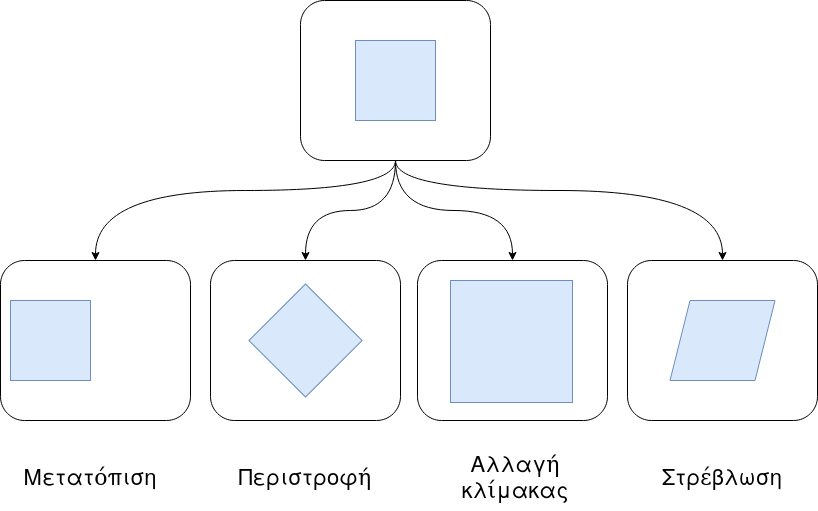
\includegraphics[width=0.7\textwidth]{affine_2}
    \captionsetup{width=0.7\textwidth}
    \caption{Μετατόπιση, περιστροφή, αλλαγή κλίμακας και στρέβλωση ενός
    τετραγώνου.}
\end{figure}

Έστω $F(x): \Omega_F \subset \R^D \mapsto \R$ η σταθερή εικόνα, $M(x): \Omega_M
\subset \R^D \mapsto \R$ η κινούμενη εικόνα και $\bm{T_{\mu}}(\bm{x}): \Omega_F
\times \R^P \mapsto \Omega_M$ παραμετροποιημένος μετασχηματισμός συντεταγμένων,
όπου $\bm{\mu} \in \R^P$ αναπαριστά το διάνυσμα των παραμέτρων του
μετασχηματισμού. Επίσης $P$ είναι ο βαθμός ελευθερίας του μετασχηματισμού.

Ο αγχίγραμμος μετασχηματισμός ορίζεται ως:

\begin{equation*}
    \bm{T_{\mu}}(\bm{x}) = \bm{A}(\bm{x} - \bm{c}) + \bm{t} + \bm{c}
\end{equation*}

Όπου $\bm{t}$ είναι το διάνυσμα μετατόπισης και $\bm{c}$ το κέντρο περιστροφής.
Επίσης, ο πίνακας $\bm{A}$ πραγματοποιεί την περιστροφή, αλλαγή κλίμακας και
στρέβλωση. Το διάνυσμα παραμέτρων $\bm{\mu}$ θα αποτελείται από τα στοιχεία
$a_{ij}$ του πίνακα $\bm{A}$ και το διάνυσμα μετατόπισης $\bm{t}$. Στις δύο
διαστάσεις ο μετασχηματισμός έχει έξι βαθμούς ελευθερίας, ενώ στις τρεις έχει
δώδεκα.

\subsubsection{Γραμμική παρεμβολή} \label{reg:linear:1}

Κατά την διαδικασία του υπολογισμού της μετρικής αξιολόγησης της κατάτμησης
(όπως στη \ref{MSSD}), συγκρίνονται οι τιμές των αντίστοιχων σημείων της
σταθερής εικόνας και των μετασχηματισμένων της κινούμενης. Αυτά τα
μετασχηματισμένα σημεία της κινούμενης εικόνας μπορεί να μην ανήκουν στο πλέγμα
της εικόνας. Γι᾽ αυτόν τον λόγο, είναι απαραίτητη η παρεμβολή των σημείων αυτών.

Η γραμμική παρεμβολή υπολογίζει τον σταθμισμένο μέσο όρο των γειτονικών
εικονοστοιχείων, χρησιμοποιώντας την απόσταση ως το βάρος.

\subsubsection{Χώρος κλίμακας Gauss} \label{reg:gauss:1}

Ένα πρόβλημα που συναντάται όσο αυξάνεται ο χώρος αναζήτησης της κατάτμησης,
είναι ότι υπάρχουν μεγαλύτερες πιθανότητες να καταλήξει η βελτιστοποίηση σε
κάποιο τοπικό ελάχιστο, με αποτέλεσμα να μην είναι καλό το αποτέλεσμα της. Ένας
τρόπος να αυξηθεί η πιθανότητα να βρεθεί το ολικό ελάχιστο είναι να
χρησιμοποιηθεί μία ιεραρχική διαδικασία κατά την οποία η πληροφορία των εικόνων
θα αυξάνεται από τα αρχικά προς τα τελικά στάδια. 

Ο χώρος κλίμακας Gauss είναι ένας τρόπος να επιτευχθεί το παραπάνω αποτέλεσμα
\cite{scale_space:1}. Αυτή η μέθοδος χρησιμοποιεί τον πυρήνα Gauss για να
μειώσει την πληροφορία μίας εικόνας. Ο πυρήνας Gauss ορίζεται για τρεις
διαστάσεις ως:

\begin{equation} \label{gaussian_kernel:1}
    g(x,y,z,t) = \frac{1} {2 \pi t} e^{\frac{-(x^2 + y^2 + z^2) }{t}}
\end{equation}

Όπου $\sqrt{2t}$ είναι η τυπική απόκλιση του πυρήνα και $t$ το επίπεδο του χώρου
κλίμακας. Ο πυρήνας αυτός συνελίσεται με μία εικόνα ώστε να μειωθεί η πληροφορία
της. Αυτό γίνεται σε πολλαπλά ιεραρχικά στάδια, στα οποία αρχικά η τιμή του $t$
είναι μεγάλη και μειώνεται σε κάθε στάδιο. Ιδανικά με αυτήν την μέθοδο, οι
εικόνες θα έχουν ένα ελάχιστο στο αρχικό ιεραρχικό επίπεδο, το οποίο θα είναι
κοντά στο επιθυμητό ολικό ελάχιστο. Έπειτα σε κάθε στάδιο αφού αυξάνεται η
πληροφορία, το ελάχιστο ιδανικά θα τείνει όλο και πιο κοντά στο ολικό.

Στο \autoref{fig:tGauss} παρουσιάζεται η ίδια εικόνα για διάφορες τιμές του $t$.
Από το σχήμα αυτό, παρατηρείται ότι όσο αυξάνεται η τιμή του $t$ τόσο μειώνεται
και η πληροφορία στην εικόνα.

\begin{figure}[H]
    \centering

    \begin{subfigure}[b]{0.4\linewidth}
    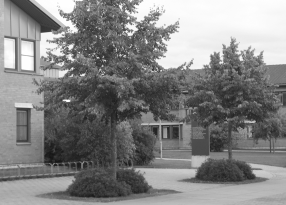
\includegraphics[width=\linewidth]{Scalespace0.png}
    \caption{$t=0$}
    \end{subfigure}
    \begin{subfigure}[b]{0.4\linewidth}
    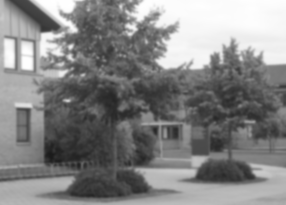
\includegraphics[width=\linewidth]{Scalespace1.png}
    \caption{$t=0.5$}
    \end{subfigure}

    \begin{subfigure}[b]{0.4\linewidth}
    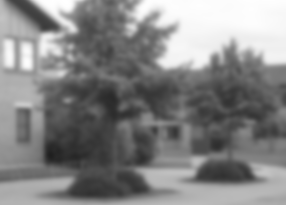
\includegraphics[width=\linewidth]{Scalespace2.png}
    \caption{$t=2$}
    \end{subfigure}
    \begin{subfigure}[b]{0.4\linewidth}
    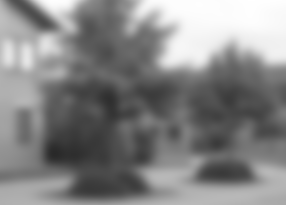
\includegraphics[width=\linewidth]{Scalespace3.png}
    \caption{$t=8$}
    \end{subfigure}

    \begin{subfigure}[b]{0.4\linewidth}
    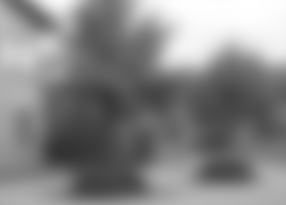
\includegraphics[width=\linewidth]{Scalespace4.png}
    \caption{$t=32$}
    \end{subfigure}
    \begin{subfigure}[b]{0.4\linewidth}
    
\includegraphics[width=\linewidth]{Scalespace5.png}
    \caption{$t=128$}
    \end{subfigure}

    \caption{Χώρος κλίμακας Gauss για διάφορες τιμές του $t$.}
    \label{fig:tGauss}
\end{figure}

\subsubsection{Δειγματοληψία συντεταγμένων εικόνας} \label{reg:sampling:1}

Κατά την διαδικασία της αξιολόγησης μπορεί να χρησιμοποιηθεί η διαδικασία της
δειγματοληψίας συντεταγμένων εικόνας ώστε να μειωθεί ο υπολογιστικός χρόνος που
χρειάζεται για την αξιολόγηση. Στην διαδικασία αυτή επιλέγονται τυχαίες
συντεταγμένες (σημεία στον χώρο της εικόνας) με ομοιόμορφη κατανομή, ώστε να
χρησιμοποιηθούν για την αξιολόγηση. Μέσω παρεμβολής των συντεταγμένων αυτών
δημιουργείται η νέα δειγματοληπτημένη εικόνα.

\subsubsection{Μάσκα εικόνας} \label{reg:mask:1}

Αν μία εικόνα (είτε σταθερή, είτε κινούμενη) έχει περιοχές στις οποίες δεν
υπάρχουν χαρακτηριστικά ενδιαφέροντος, τότε μπορεί να χρησιμοποιηθεί μία μάσκα
εικόνας, ώστε μην να συμπεριληφθούν οι περιοχές αυτές στην διαδικασία της
κατάτμησης. Η μάσκα εικόνας είναι μία δυαδική εικόνα, η οποία υποδεικνύει εάν
ένα εικονοστοιχείο θα συμπεριληφθεί στην διαδικασία της κατάτμησης. Το μέγεθος
της μάσκας είναι ίδιο με το μέγεθος της εικόνας που θα εφαρμοστεί, ώστε να
υπάρχει αντιστοιχία μεταξύ των εικονοστοιχείων της εικόνας και των
εικονοστοιχείων της μάσκας. Επομένως, κάθε εικονοστοιχείο της μάσκας δηλώνει εάν
το αντίστοιχο εικονοστοιχείο της εικόνας θα χρησιμοποιηθεί στην κατάτμηση.

\subsection{Μέτρα αξιολόγησης}

Τα μέτρα αξιολόγησης χρησιμοποιούνται για να αξιολογήσουν το αποτέλεσμα της
κατάτμησης. Συγκρίνουν το αποτέλεσμα της κατάτμησης με το επιθυμητό αποτέλεσμα,
ούτως ώστε να παράξουν μία αριθμητική αναπαράσταση της ποιότητας της κατάτμησης.
Με αυτόν το τρόπο μπορούν να συγκριθούν διαφορετικοί αλγόριθμοι κατάτμησης και
διαφορετικές τιμές για τον ίδιο αλγόριθμο.

Η επιλογή του μέτρου ή των μέτρων αξιολόγησης έχει μεγάλη σημασία για την
δημιουργία και τον συντονισμό (επιλογή των κατάλληλων μεταβλητών) του μοντέλου
επειδή, είναι το μέτρο που θα χρησιμοποιηθεί για την επιλογή του καταλληλότερου
μοντέλου. Η επιλογή αυτή ταυτίζεται με την επιθυμητή συμπεριφορά του τελικού
μοντέλου. Για παράδειγμα, αν το επιθυμητό μοντέλο πρέπει να έχει όσο είναι
δυνατόν πιο λίγα αληθή αρνητικά, τότε πρέπει να επιλεχθεί και το ανάλογο μέτρο
αξιολόγησης που να ικανοποιεί τον περιορισμό αυτό.

\subsubsection{Συντελεστής ομοιότητας Dice} \label{Dice:1}

Ο συντελεστής ομοιότητας Dice είναι μία μετρική που εκτιμά την ομοιότητα μεταξύ
δύο συνόλων \cite{dice:1}. Είναι γνωστός επίσης και ως δείκτης Sørensen–Dice,
συντελεστής Dice και F1 σκορ. Ο συντελεστής ομοιότητας Dice ορίζεται ως:

\begin{equation} \label{eq:Dice:1}
    DSC = \frac{2 \abs{X \cap Y}} {\abs{X} + \abs{Y}}
\end{equation}

Όπου $X$ και $Y$ είναι σύνολα, $\abs{x}$ είναι ο αριθμός των στοιχείων του
συνόλου $x$ και $\cap$ δηλώνει την τομή δύο συνόλων.

Στην αξιολόγηση της κατάτμησης εικόνας τα παραπάνω σύνολα αποτελούνται από το
σύνολο των εικονοστοιχείων που ανήκουν σε μία κλάση. Επομένως ο συντελεστής
αυτός υπολογίζει το ποσοστό των σημείων μίας κλάσης που επικαλύπτονται. Η
μέγιστη τιμή του συντελεστή είναι $1$ και η ελάχιστη $0$.

\subsubsection{Δείκτης δομικής ομοιότητας} \label{SSIM:1}

Ο δείκτης δομικής ομοιότητας \cite{SSIM:1} (Structural SIMilarity index, SSIM)
είναι μία μετρική της ομοιότητας δύο εικόνων. Χρησιμοποιεί τις σύγκρισεις της
φωτεινότητας, της αντίθεσης και της δομής των εικόνων. Κατά την δημιουργία μίας
εικόνας η φωτεινότητα των αντικειμένων της εικόνας εξαρτάται από τον φωτισμό και
την ανακλαστικότητα των αντικειμένων αυτών, αλλά και από την δομής τους. Γι᾽
αυτό τον λόγο είναι επιθυμητό να διαχωριστεί η επίδραση της φωτεινότητας έτσι
ώστε η δομή να είναι ανεξάρτητη από την φωτεινότητα. Επομένως μπορεί να οριστεί
η δομική πληροφορία της εικόνας ως τα χαρακτηριστικά των αντικειμένων της που
είναι ανεξάρτητα από την φωτεινότητα και την αντίθεση.

Η φωτεινότητα ενός σήματος ορίζεται ως:

\begin{equation}\label{luminance}
    \mu_x = \frac {1} {N} \sum_{i=1}^{N} x_i
\end{equation}

Όπου $x$ είναι το σήμα  και $N$ ο αριθμός των στοιχείων του. Αν οι τιμές των
εικονοστοιχείων μίας εικόνας τοποθετηθούν σε ένα διάνυσμα τότε μπορεί να
χρησιμοποιηθεί ο τύπος \eqref{luminance} για τον υπολογισμό της φωτεινότητας
αλλά και των παρακάτω τύπων. Για να αφαιρεθεί η επίδραση της φωτεινότητας στο
σήμα θα πρέπει να ισχύει:

\begin{equation*}
    \sum_{i=1}^{N} x_i = 0
\end{equation*}

Η αντίθεση της σήματος-εικόνας εκτιμάτε με την διακύμανση του σήματος:

\begin{equation*}
    \sigma_x = \sqrt{\left(\, \frac{1}{N-1} \sum_{i=1}^{N} {\left(\,x_i -
                     \mu_x\right)}^2\, \right)}
\end{equation*}

Για να αφαιρεθεί και η επίδραση της αντίθεσης θα πρέπει να κανονικοποιηθεί το
σήμα, δηλαδή να διαιρεθεί με την διακύμανση του ώστε να έχει μοναδιαία
διακύμανση. Επομένως

\begin{equation*}
    \hat{x} = \frac{x-\mu_x} {\sigma_x}
\end{equation*}

Όπου $\hat{x}$ είναι το κανονικοποιημένο σήμα. Η σύγκριση της φωτεινότητας δύο
εικόνων $x$ και $y$ ορίζεται ως:

\begin{equation}\label{luminance_comp}
    l(x,y) = \frac {2\mu_x\mu_y + C_1} {\mu_x^2 + \mu_y^2 + C_1}
\end{equation}

Η σταθερά $C_1$ μπορεί να χρησιμοποιηθεί για να αποφευχθεί υπολογιστική αστάθεια
για μικρές τιμές του παρανομαστή. Η σύγκριση της αντίθεσης ορίζεται ως:

\begin{equation}\label{contrast_comp}
    c(x,y) = \frac {2\sigma_x\sigma_y + C_2} {\sigma_x^2 + \sigma_y^2 + C_2}
\end{equation}

Όπου η σταθερά $C_2$ χρησιμοποιείται επίσης για την υπολογιστική σταθερότητα.
Επειδή η συσχέτιση των κανονικοποιημένων σημάτων $\hat{x}$ και $\hat{y}$ είναι
ίδια με την συσχέτιση των μη κανονικοποιημένων σημάτων, μπορεί να οριστεί η
σύγκριση της δομής (που είναι ανεξάρτητη από την φωτεινότητα και την αντίθεση)
ως:

\begin{equation}\label{structure_comp}
    s(x,y) = \frac {\sigma_{xy} + C_3} {\sigma_x \sigma_y + C_3}
\end{equation}

Όπου η σταθερά $C_3$ χρησιμοποιείται επίσης για την υπολογιστική σταθερότητα και
$\sigma_{xy}$ είναι η συνδιακύμανση των σημάτων και ορίζεται ως:

\begin{equation*}
    \sigma_{xy} = \frac {1} {N-1} \sum_{i=1}^{N} {(x_i - \mu_x) (y_i - \mu_y)}
\end{equation*}

Τέλος, χρησιμοποιώντας τις συγκρίσεις της φωτεινότητας, της αντίθεσης και της
δομής (\eqref{luminance_comp}, \eqref{contrast_comp} και \eqref{structure_comp}
αντίστοιχα), ο τύπος του δείκτης δομικής ομοιότητας ορίζεται ως:

\begin{equation} \label{eq:SSIM:1}
    SSIM(x,y) = \left[l(x,y)\right]^\alpha \left[c(x,y)\right]^\beta 
                \left[s(x,y)\right]^\gamma
\end{equation}

Οι τιμές $\alpha$, $\beta$ και $\gamma$ χρησιμοποιούνται για να ορίσουν την
επίδραση κάθε σύγκρισης.

\subsection{Προεπεξεργασία δεδομένων} \label{preprocessing:1}

Η προεπεξεργασία των δεδομένων αποτελεί ένα από τα πιο βασικά βήματα της
μηχανικής μάθησης. Σε αυτό το βήμα τα δεδομένα αναλύονται και επεξεργάζονται
ούτως ώστε η διαδικασία της μάθησης να είναι πιο αποτελεσματική. Αν τα δεδομένα
περιέχουν περιττές και ασυσχέτιστες πληροφορίες για το πρόβλημα που
χρησιμοποιούνται, τότε δυσκολεύουν την διαδικασία της μάθησης. Το ίδιο ισχύει
και για αφερέγγυα και θορυβώδη δεδομένα. Επίσης στην προεπεξεργασία μπορεί να
αυξηθεί η σημαντικότητα μερικών χαρακτηριστικών των δεδομένων.

Στη περίπτωση όπου τα δεδομένα αποτελούνται από εικόνες-απεικονίσεις, σκοπός της
προεπεξεργασίας είναι να παραχθεί μία νέα εικόνα-απεικόνιση που θα έχει καλύτερα
αποτελέσματα στην μάθηση από αυτά της αρχικής. Πιο αναλυτικά, σκοπεύει στην
εξάλειψη της αθέμιτης διαστρέβλωσης των εικόνων, στην αύξηση της σημαντικότητας
μερικών χαρακτηριστικών τους και στον γεωμετρικός μετασχηματισμός τους
\cite{Image_preprocessing:1}.

\iffalse
Οι μέθοδοι προεπεξεργασίας
δεδομένων εικόνας μπορούν να διαχωριστούν σε τέσσερις κατηγορίες ανάλογα με την
γειτονία των εικονοστοιχείων που χρησιμοποιείται για τον υπολογισμό της νέας
εικόνας, όπως παρουσιάζεται στο \cite{Image_preprocessing:1}. Οι κατηγορίες
αυτές είναι:

\begin{enumerate}
    \item Μέθοδοι που επεξεργάζονται την ένταση κάθε εικονοστοιχείου ξεχωριστά.
    \item Γεωμετρική μετασχηματισμοί.
    \item Μέθοδοι που χρησιμοποιούν πληροφορίες των γειτονικών εικονοστοιχείων.
    \item 
\end{enumerate}
\fi

\subsubsection{Αντιστοίχιση ιστογράμματος} \label{histogram:1}

Η αντιστοίχιση ιστογράμματος είναι ένας μετασχηματισμός της εικόνας κατά τον
οποίο το ιστόγραμμα της εικόνας αντιστοιχίζεται με ένα άλλο ιστόγραμμα το οποίο
μπορεί να προέρχεται από άλλη εικόνα. Αυτό μπορεί να επιτευχθεί με διάφορους
αλγόριθμους. Ο αλγόριθμος που θα παρουσιαστεί περιγραφικά παρακάτω βασίζεται στο
\cite{histogram_matching:1}.

Ο αλγόριθμος πραγματοποιεί γραμμικούς μετασχηματισμούς για διάφορα τμήματα του
ιστογράμματος των εικόνων. Αρχικά υπολογίζει τα τμήματα αυτά μέσω
προκαθορισμένων τιμών της συνάρτησης αθροιστικής κατανομής. Έπειτα υπολογίζει
για κάθε άκρο τον μέσο όρο των αντίστοιχων τιμών. Τέλος μετασχηματίζει γραμμικά
τις τιμές κάθε εικόνας, για κάθε διάστημα, από το αρχικό διάστημα της εικόνας,
στο τελικό διάστημα που υπολογίστηκε με τον μέσο όρο.

Στο \autoref{fig:histogram_matching} φαίνεται η διαδικασία τους γραμμικού
μετασχηματισμού μίας εικόνας. Οι τιμές της εικόνας μετασχηματίζονται γραμμικά
από τον οριζόντιο άξονα στον κάθετο. Στο παράδειγμα αυτό υπάρχουν τέσσερα
διαστήματα, όπου $\mu_1, \mu_2, \mu_3, \mu_4$ είναι τα άκρα του αρχικού
διαστήματος και $\mu_{s1}, \mu_{s2}, \mu_{s3}, \mu_{s4}$ τα άκρα του τελικού.
$m_1, m_2$ είναι η ελάχιστη και η μέγιστη τιμή αντίστοιχα της εικόνας και
$m_{s1}, m_{s2}$ ίδια άκρα για το αποτέλεσμα της αντιστοίχισης ιστογράμματος.

\begin{figure}[H]
    \centering
    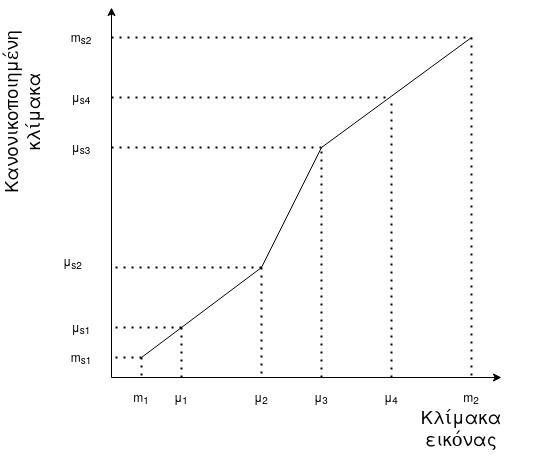
\includegraphics[width=0.6\textwidth]{histogram_matching_2}
    \iffalse
    \caption{Γραμμικός μετασχηματισμός μίας εικόνας για τέσσερα άκρα. $\mu_1,
             \mu_2, \mu_3, \mu_4$ είναι τα άκρα του αρχικού διαστήματος και
             $\mu_{s1}, \mu_{s2}, \mu_{s3}, \mu_{s4}$ τα άκρα του τελικού. $m_1,
             m_2$ είναι η ελάχιστη και η μέγιστη τιμή αντίστοιχα της εικόνας και
             $m_{s1}, m_{s2}$ ίδια άκρα για το αποτέλεσμα της αντιστοίχισης
             ιστογράμματος.}
    \fi
    % \captionsetup{width=0.7\textwidth}
    \caption{Γραμμικός μετασχηματισμός αντιστοίχισης ιστογράμματος μίας εικόνας
             για τέσσερα άκρα.}
    \label{fig:histogram_matching}
\end{figure}

\subsubsection{Απαλοιφή θορύβου εικόνας μέσω ροής της καμπυλότητας}
\label{curvature_flow:1}

Η ροή της καμπυλότητας μπορεί να χρησιμοποιηθεί για την απαλοιφή του θορύβου.
Συγκεκριμένα, σε μία μία εικόνα χρησιμοποιούνται οι καμπύλες που σχηματίζονται
από τα εικονοστοιχεία που έχουν την ίδια τιμή (φωτεινότητα εικονοστοιχείου). Οι
καμπύλες αυτές εξελίσσονται \cite{curvature_flow:1} μέσω της μερικής διαφορικής
εξίσωσης:

\begin{equation} \label{eq:curvature_flow:1}
    I_t = \kappa \abs{\nabla I}
\end{equation}

Όπου $I$ είναι η εικόνα και $\kappa$ η καμπυλότητα. Η καμπυλότητα μίας καμπύλης
$\bm{\gamma}$ ορίζεται ως:

\begin{equation*}
    \kappa = \frac {\norm{\bm{\gamma}' \times \bm{\gamma}''}}
                   {\norm{\bm{\gamma}'}^3}
\end{equation*}

Όπου το σύμβολο $x'$ δηλώνει την παράγωγο της συνάρτησης $x$ ως προς τον χρόνο.
Επίσης $\norm{v}$ είναι η ευκλείδεια νόρμα του διανύσματος $v$.

Αυτή η τεχνική για την απαλοιφή του θορύβου έχει το πλεονέκτημα ότι διατηρεί
τα αιχμηρά όρια της εικόνας ενώ ταυτόχρονα εξομαλύνει τα υπόλοιπα σημεία. Επειδή
οι ροή των καμπυλών τείνει προς την εξάλειψη των ορίων, η υπερβολική χρήση της
τεχνική θα οδηγήσει στη εξάλειψη της πληροφορίας στη εικόνα.

\subsection{Διασταυρωμένη επικύρωση}

Σύμφωνα με το \cite{cross_validation:1}, διασταυρωμένη επιτήρηση είναι μια
στατιστική μέθοδος αξιολόγησης και σύγκρισης των αλγορίθμων μάθησης διαιρώντας
τα δεδομένα σε δύο τμήματα. Το ένα χρησιμοποιείται για την εκμάθηση ή την
εκπαίδευση ενός μοντέλου και το άλλο χρησιμοποιείται για την επικύρωση του
μοντέλου. Ο σκοπός της διασταυρωμένης επικύρωσης είναι μέσω αυτής να αξιολογηθεί
η δυνατότητα του μοντέλου να πραγματοποιεί σωστές προβλέψεις για δεδομένα που
δεν χρησιμοποιήθηκαν για την εκπαίδευση του. Έτσι μπορεί να κριθεί η ικανότητα
του μοντέλου να γενικεύει (ικανότητα πρόβλεψης του σε ανεξάρτητα δεδομένα).

\subsubsection{Αφήνω ένα έξω διασταυρωμένη επικύρωση} \label{leave_one_out:1}

Η μέθοδος αφήνω ένα έξω διασταυρωμένης επικύρωσης είναι μία μέθοδος
διασταυρωμένης επικύρωσης κατά την οποία χρησιμοποιείται μία παρατήρηση από το
σύνολο των δεδομένων για την επικύρωση του μοντέλου και οι υπόλοιπες για την
εκπαίδευση του. Η διαδικασία αυτή επαναλαμβάνεται μέχρις ότου κάθε παρατήρηση
του συνόλου δεδομένων έχει χρησιμοποιηθεί για την επικύρωση. Αν $\bm{m}$ είναι ο
συνολικός αριθμός των παρατηρήσεών, τότε η διαδικασία αυτή επαναλαμβάνεται
$\bm{m}$ φορές.

\iffalse
NOTES:
    !Graph-Based Framework for Label Fusion 
    !lasso
    !registration
    !dice, (maybe) sse
    !structural similarity measure (SSIM)
    !φιλτρα
    !leave-one-out cross validation
\fi


\section{Μέθοδοι επίλυσης του προβλήματος}

Σε αυτό το κεφάλαιο θα παρουσιαστούν οι μέθοδοι επίλυσης του προβλήματος. Όπως
προαναφέρθηκε, το πρόβλημα αφορά την κατάτμηση ιατρικών απεικονίσεων βάση
ατλάντων με χρήση μεθόδων μηχανικής μάθησης. Οι ιατρικές απεικονίσεις
αποτελούνται από απεικονίσεις μαγνητικής τομογραφίας γονάτων.

\subsection{Δεδομένα} \label{data:1}

Τα δεδομένα που χρησιμοποιήθηκαν τόσο για την εκπαίδευση των μοντέλων όσο και
για την αξιολόγηση τους προέρχονται από το OAI ZIB. Συγκεκριμένα τα δεδομένα
αυτά αποτελούνται από απεικονίσεις μαγνητικής τομογραφίας γονάτων μαζί με τις
αντίστοιχες κατατμήσεις τους. Η κατάτμηση έχει γίνει χειροκίνητα από ειδικούς.
Οι κλάσεις της κατάτμησης αποτελούνται από τα οστά, τους χόνδρους και το
υπόβαθρο.  Χρησιμοποιήθηκαν 46 από τα 507 δείγματα που διατίθενται. Τα δεδομένα
που χρησιμοποιήθηκαν καλύπτουν όλο το φάσμα του βαθμού οστεοαρθρίτιδας. Στον
\autoref{dataset:1} απαριθμούνται κάποια χαρακτηριστικά των δεδομένων της βάσης
OAI ZIB.

\begin{table}[h!]
    \centering
    \begin{tabular}{|c|c|} 
        \hline
        MRI scanner            & Siemens 3T Trio \\ 
        MRI sequence           & DESS            \\
        Acquisition plane      & Sagittal        \\
        Image resolution in mm & 0.36×0.36×0.7   \\
        Timepoints             & Baseline        \\
        \hline
    \end{tabular}
    \caption{Χαρακτηριστικά δεδομένων OAI ZIB.}
    \label{dataset:1}
\end{table}

Οι κλάσεις-ετικέτες των δεδομένων που χρησιμοποιήθηκαν για την κατάτμηση μαζί με
την τιμή τους είναι:

\begin{enumerate}
    \setcounter{enumi}{-1} 
    \item Υπόβαθρο
    \item Οστό
    \item Χόνδρος
\end{enumerate}

\subsection{Προεπεξεργασία δεδομένων}

Όπως αναφέρθηκε και στο \ref{preprocessing:1}, σκοπός της προεπεξεργασίας είναι
να παραχθεί μία νέα εικόνα-απεικόνιση που θα έχει καλύτερα αποτελέσματα στην
μάθηση από αυτά της αρχικής. Με τις μεθόδους που παρουσιάζονται παρακάτω
επιθυμείτε να υπάρξει το αποτέλεσμα αυτό που θα βοηθήσει στην διαδικασία την
εκμάθησης.

\subsubsection{Απαλοιφή θορύβου εικόνας μέσω ροής της καμπυλότητας}

Κατά την προεπεργασία των απεικονίσεων χρησιμοποιήθηκε αρχικά η απαλοιφή θορύβου
εικόνας μέσω ροής της καμπυλότητας (\ref{curvature_flow:1}). Με την μέθοδο αυτή
επιτυγχάνεται η μύωση του θορύβου στις απεικονίσεις και η διατήρηση-τόνωση των
αιχμηρών σημείων (σημείων που διαχωρίζονται οι διάφορες ανατομικές περιοχές) των
απεικονίσεων.

Η τιμή που χρησιμοποιήθηκε για το χρονικό βήμα είναι $t=0.04$ (από την εξίσωση
\eqref{eq:curvature_flow:1}) και η μέθοδος επαναλήφθηκε δέκα φορές.  Στα
\autoref{fig:curvature_flow:1}, \autoref{fig:curvature_flow:2} και
\autoref{fig:curvature_flow:3} παρουσιάζονται απεικονίσεις του ίδιου γόνατου,
από διάφορες οπτικές γωνίες, χωρίς και με την χρήση της απαλοιφής θορύβου. Από
τα σχήματα αυτά φαίνεται ότι ο θόρυβος έχει μειωθεί αρκετά. Επίσης είναι εμφανές
ότι οι ακμές των καμπυλών έχουν διατηρηθεί και σε μερικές περιπτώσεις έχουν
αυξηθεί μετά τη χρήση της μεθόδου.

\begin{figure}[H]
    \centering

    \begin{subfigure}[t]{0.4\linewidth}
    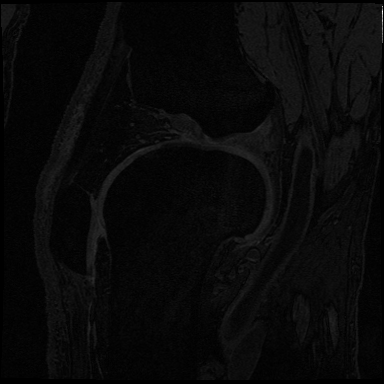
\includegraphics[width=\linewidth]{original_1.png}
    \caption{Αρχική απεικόνιση}
    \end{subfigure}
    \begin{subfigure}[t]{0.4\linewidth}
    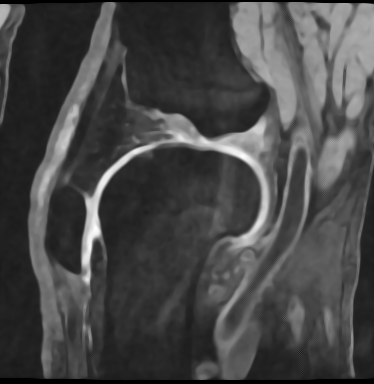
\includegraphics[width=\linewidth]{curvature_1.png}
    \caption{Απεικόνιση με απαλοιφή θορύβου}
    \end{subfigure}

    \begin{subfigure}[t]{0.4\linewidth}
    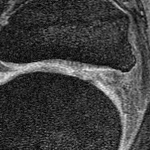
\includegraphics[width=\linewidth]{original_1_1.png}
    \caption{Μεγέθυνση της αρχικής απεικόνιση}
    \end{subfigure}
    \begin{subfigure}[t]{0.4\linewidth}
    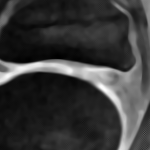
\includegraphics[width=\linewidth]{curvature_1_1.png}
    \caption{Μεγέθυνση της απεικόνισης με απαλοιφή θορύβου}
    \end{subfigure}

    \caption{Τομή απεικόνισης γονάτου χωρίς και με την χρήση της απαλοιφής
    θορύβου μέσω ροής της καμπυλότητας.}
    \label{fig:curvature_flow:1}
\end{figure}

\begin{figure}[H]
    \centering
    \begin{subfigure}[t]{0.4\linewidth}
    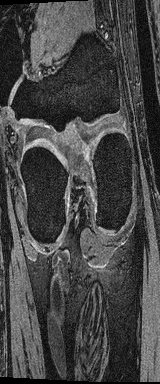
\includegraphics[width=\linewidth]{original_2.png}
    \caption{Αρχική απεικόνιση}
    \end{subfigure}
    \begin{subfigure}[t]{0.4\linewidth}
    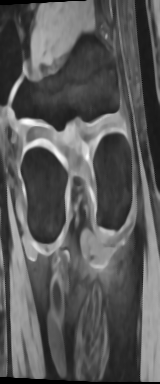
\includegraphics[width=\linewidth]{curvature_2.png}
    \caption{Απεικόνιση με απαλοιφή θορύβου}
    \end{subfigure}

    \caption{Τομή απεικόνισης γονάτου χωρίς και με την χρήση της απαλοιφής
    θορύβου μέσω ροής της καμπυλότητας.}
    \label{fig:curvature_flow:2}
\end{figure}

\begin{figure}[H]
    \centering
    \begin{subfigure}[t]{0.4\linewidth}
    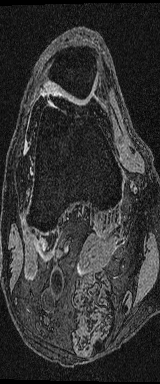
\includegraphics[width=\linewidth]{original_3.png}
    \caption{Αρχική απεικόνιση}
    \end{subfigure}
    \begin{subfigure}[t]{0.4\linewidth}
    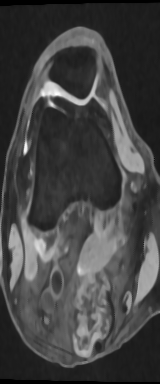
\includegraphics[width=\linewidth]{curvature_3.png}
    \caption{Απεικόνιση με απαλοιφή θορύβου}
    \end{subfigure}

    \caption{Τομή απεικόνισης γονάτου χωρίς και με την χρήση της απαλοιφής
    θορύβου μέσω ροής της καμπυλότητας.}
    \label{fig:curvature_flow:3}
\end{figure}


\subsubsection{Αντιστοίχιση ιστογράμματος}

Έπειτα από την απαλοιφή του θορύβου χρησιμοποιήθηκε η αντιστοίχιση ιστογράμματος
(\ref{histogram:1}). Το ιστόγραμμα της κινούμενης απεικόνισης αντιστοιχίστηκε με
το ιστόγραμμα της σταθερής απεικόνισης. Σκοπός του μετασχηματισμού αυτού είναι
οι απεικονίσεις να έχουν την ίδια φωτεινότητα για τις αντίστοιχες βιολογικές
περιοχές των γονάτων στην σταθερή και στην κινούμενη απεικόνιση. 
% Με αυτόν τον τρόπο θα είναι πιο εύκολη η διαδικασία της κατάτμησης.

Αν και οι απεικονίσεις προέρχονται από το ίδιο μοντέλο μαγνητικού τομογράφου,
μπορούν να παρουσιάζουν μεταβολές στην φωτεινότητα τους. Γι᾽ αυτό το λόγο
χρησιμοποιείται η αντιστοίχιση ιστογράμματος.

Στο \autoref{fig:histogram_matching:1} παρουσιάζονται τα ιστογράμματα μίας
απεικόνισης πριν και μετά την διαδικασία της αντιστοίχισης. Επίσης παρουσιάζεται
και το ιστόγραμμα της σταθερή απεικόνισης. Από το διάγραμμα αυτό φαίνεται ότι η
μεγάλη ακμή της κινούμενης απεικόνισης μετακινήθηκε προς την ακμή της σταθερής.
Επίσης παρατηρείται ολόκληρη η καμπύλη της κινούμενης απεικόνισης να ακολουθεί
την μεταβολή της ακμής της. Ακόμα από το \autoref{fig:histogram_matching:2}
δεν μπορεί να παρατηρηθεί με το μάτι διαφορά στην απεικόνιση της κινούμενης
εικόνας πριν και μετά την αντιστοίχιση του ιστογράμματος. Το γεγονός αυτό είναι
αναμενόμενο αφού η μεταβολή του ιστογράμματος δεν είναι μεγάλη όπως φαίνεται από
το \autoref{fig:histogram_matching:1}.


\begin{figure}[H]
    \centering
    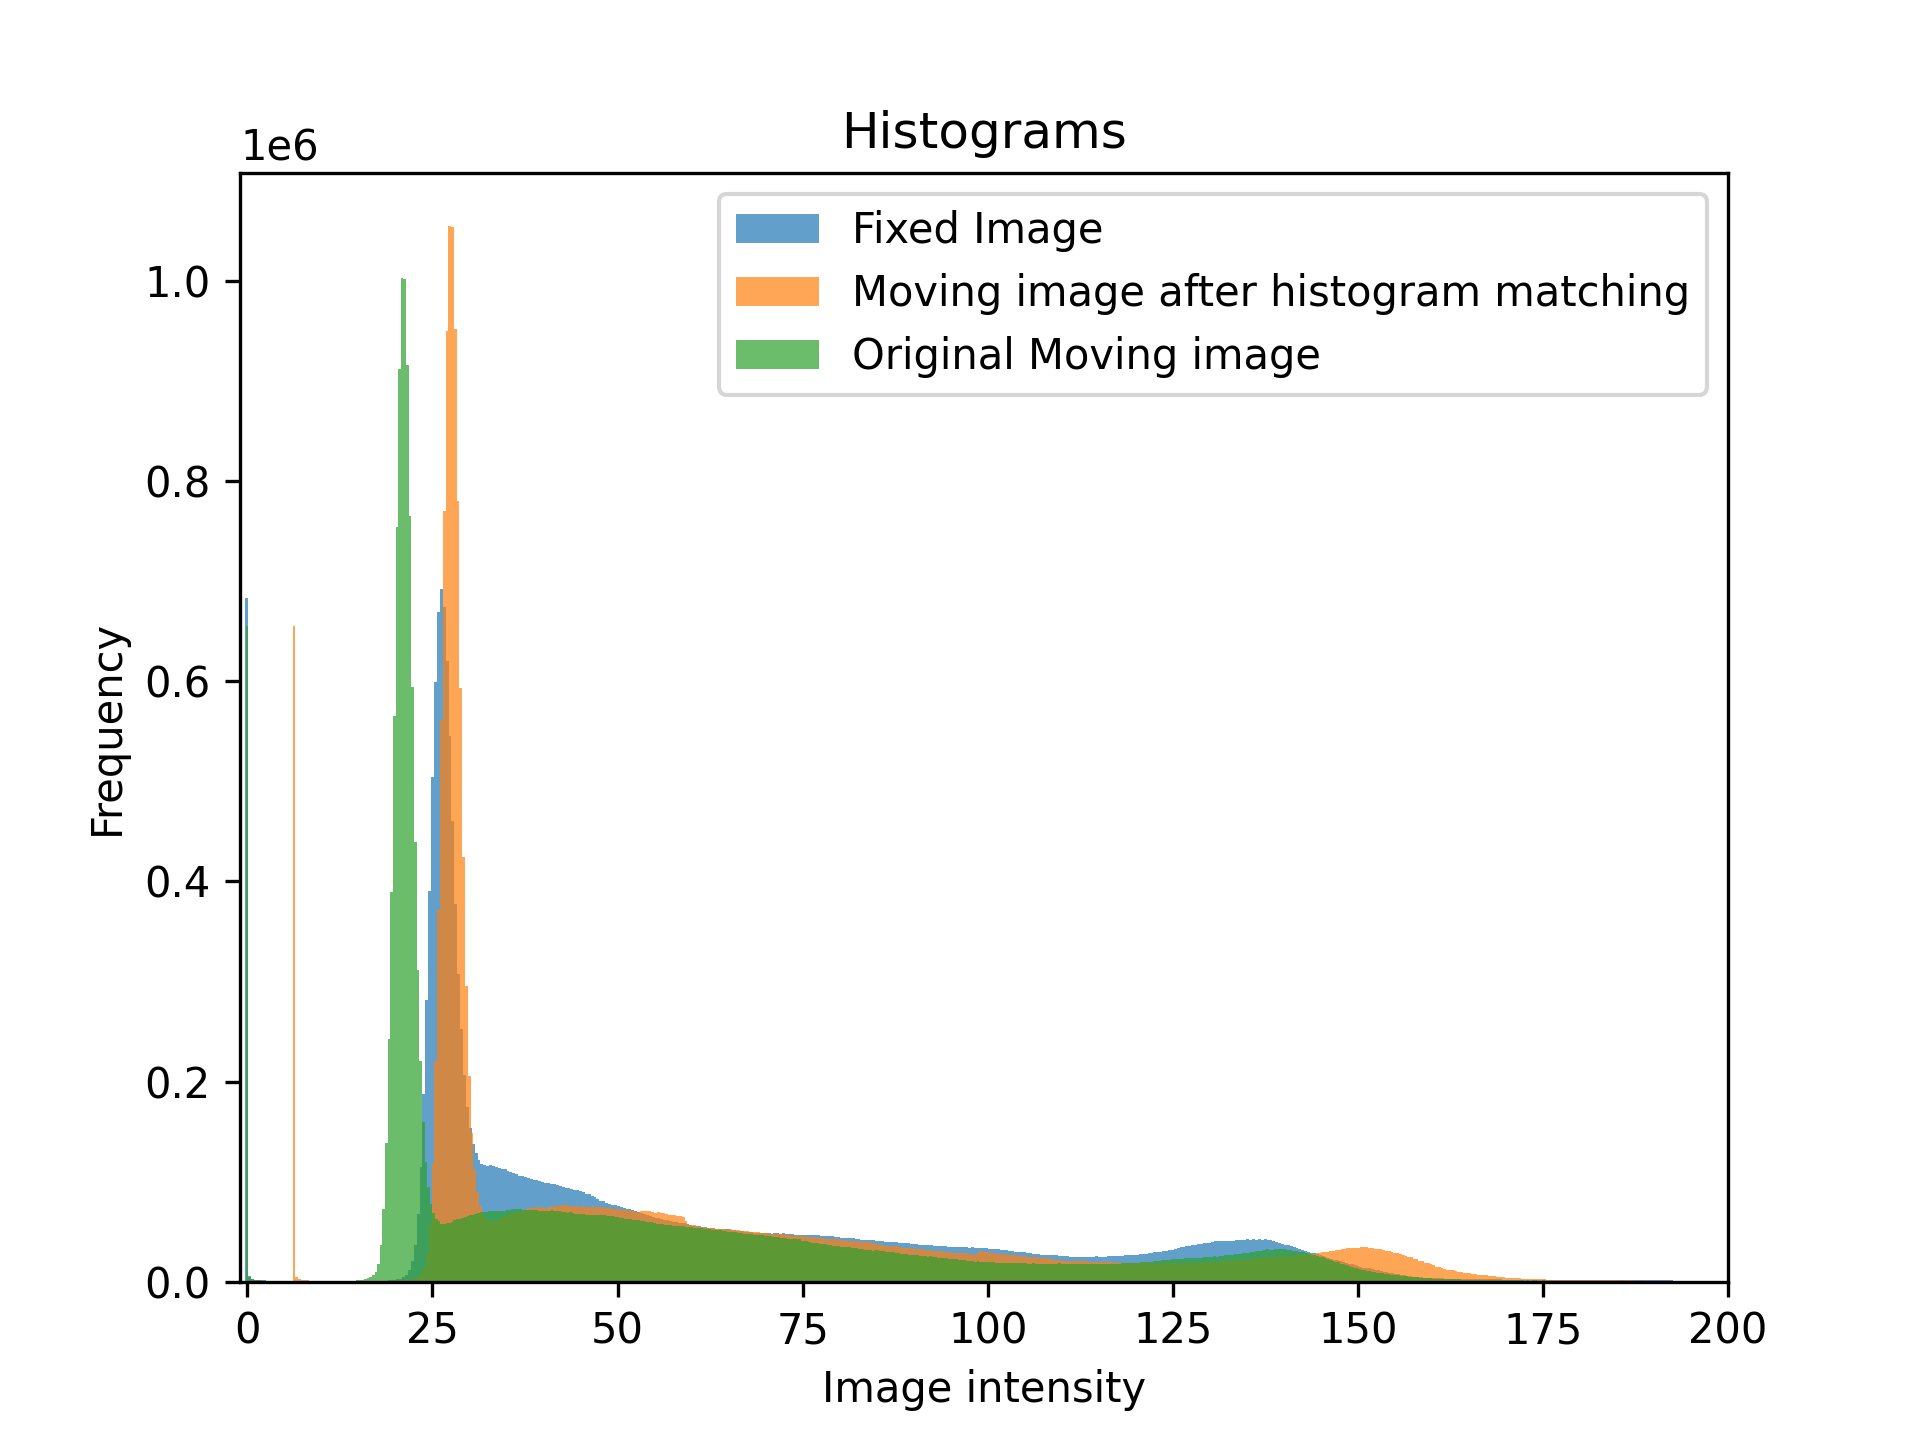
\includegraphics[width=\linewidth]{histogram_plot.png}
    \caption{Ιστογράμματα σταθερής απεικόνισης και κινούμενης πριν και μετά την
             αντιστοίχιση}
    \label{fig:histogram_matching:1}
\end{figure}


\begin{figure}[H]
    \centering

    \begin{subfigure}[t]{0.4\linewidth}
    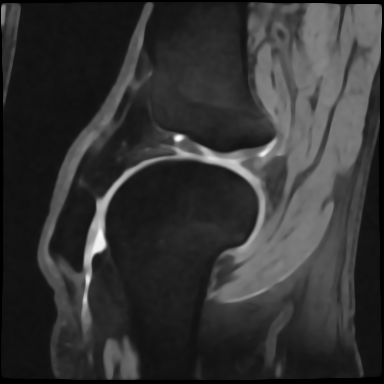
\includegraphics[width=\linewidth]{original_moving_1.png}
    \caption{Κινούμενη απεικόνιση πριν της αντιστοίχιση ιστογράμματος}
    \end{subfigure}
    \begin{subfigure}[t]{0.4\linewidth}
    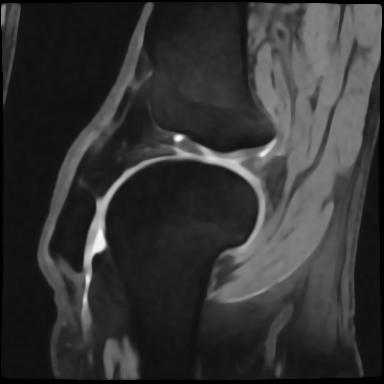
\includegraphics[width=\linewidth]{original_moving_histogram_matching_1.png}
    \caption{Κινούμενη απεικόνιση πριν της αντιστοίχιση ιστογράμματος}
    \end{subfigure}

    \begin{subfigure}[t]{0.4\linewidth}
    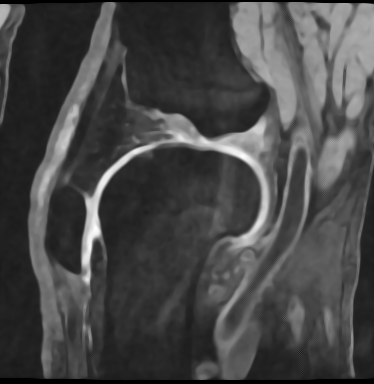
\includegraphics[width=\linewidth]{curvature_1.png}
    \caption{Σταθερή απεικόνιση}
    \end{subfigure}

    \caption{Τομή απεικονίσεων σταθερή και κινούμενης εικόνας πριν και μετά την
             αντιστοίχιση ιστογράμματος.}
    \label{fig:histogram_matching:2}
\end{figure}


\subsection{Καταχώρηση απεικονίσεων}

Πριν την κατάτμηση των απεικονίσεων είναι απαραίτητο να καταχωρηθούν οι
απεικονίσεις των ατλάντων που θα χρησιμοποιηθούν για την κατάτμηση της σταθερής
απεικόνισης. Άτλας είναι ο συνδυασμός μίας απεικόνισης και του αντίστοιχου χάρτη
των ετικετών της απεικόνισης. Όπως αναφέρθηκε στο \ref{registration:1}, μέσω της
καταχώρησης επιδιώκεται τα κοινά χαρακτηριστικά των δύο απεικονίσεων (σταθερή
και κινούμενη) να επικαλυφθούν. Με αυτό τον τρόπο αντίστοιχα εικονοστοιχεία των
δύο απεικονίσεων θα αναπαριστούν όμοια βιολογικά σημεία.

Για την διαδικασία την καταχώρησης χρησιμοποιήθηκε ο αγχίγραμμος μετασχηματισμός
(\ref{reg:affine:1}). Επίσης η μέτρηση της ομοιότητας των δύο απεικονίσεων έγινε
με την μέση διαφορά τετραγώνων (\ref{MSSD}), με την υπόθεση ότι όμοια βιολογικά
σημεία στις απεικονίσεις έχουν την ίδια φωτεινότητα. Ο αλγόριθμος
βελτιστοποίησης που χρησιμοποιήθηκε ώστε να βρεθούν οι βέλτιστες παράμετροι
είναι ο αλγόριθμος προσαρμοστικής στοχαστικής απότομης καθόδου
(\ref{reg:asgd:1}). Η παρεμβολή των σημείων των απεικονίσεων έγινε με γραμμική
παρεμβολή (\ref{reg:linear:1}).  Χρησιμοποιήθηκε δειγματοληψία
(\ref{reg:sampling:1}) $80\%$ του συνολικού αριθμού των εικονοστοιχείων μίας
απεικόνισης για να μειωθεί ο χρόνο υπολογισμού που απαιτείται για την
καταχώρηση.

Ο χώρος κλίμακας Gauss (\ref{reg:gauss:1}) χρησιμοποιήθηκε ούτως ώστε να
υπάρχουν μεγαλύτερες πιθανότητες να μην καταλήξει η βελτιστοποίηση σε κάποιο
ολικό ελάχιστο. Χρησιμοποιήθηκαν τέσσερα στάδια. Η τυπική απόκλιση του πυρήνα
\eqref{gaussian_kernel:1} για κάθε στάδιο ορίζεται από τον τύπο:

\begin{equation} \label{standard_deviation:1}
    \sigma = \frac {f} {2} s
\end{equation}

Όπου $f$ αναπαριστά το επίπεδο μείωσης της πληροφορίας και έχει τιμές για κάθε
στάδιο $8,4,2,1$ αντίστοιχα. $s$ είναι η απόσταση των εικονοστοιχείων της
απεικόνισης για κάθε διάσταση (μπορεί να βρεθεί στον \autoref{dataset:1}).
\iffalse
Επειδή η τιμή αυτή δεν είναι ίδια σε όλες τις διαστάσεις μπορεί να θεωρηθεί ότι
χρησιμοποιείται μονοδιάστατος πυρήνας Gauss με τυπική απόκλιση που ορίζεται από
την εξίσωση \eqref{standard_deviation:1} για κάθε διάσταση της απεικόνισης και
ορίζεται από τον τύπο:

\begin{equation*}
    g(x) = \frac {1} {\sigma\sqrt{2\pi}} \exp{\left( -\frac{1}{2}
           \frac {x^2} {\sigma^2} \right)}
\end{equation*}
\fi

Τέλος χρησιμοποιήθηκε μάσκα (\ref{reg:mask:1}) για την κινούμενη εικόνα. Η μάσκα
αυτή αποτελείται από όλα τα εικονοστοιχεία της απεικόνισης που δεν ανήκουν στο
υπόβαθρο. Με αυτόν τον τρόπο συνεισφέρουν μόνο τα εικονοστοιχεία των
απεικονίσεων που ανήκουν σε βιολογικές ομάδες που πρόκειται να κατανεμηθούν.

Στα \autoref{fig:registration_before:1}, \autoref{fig:registration_before:2} και
\autoref{fig:registration_before:3} παρουσιάζονται οι ετικέτες δύο απεικονίσεων
πριν την καταχώρηση. Στα \autoref{fig:registration_after:1},
\autoref{fig:registration_after:2} και \autoref{fig:registration_after:3}
παρουσιάζονται οι αντίστοιχες ετικέτες μετά την καταχώρηση. Από τα σχήματα αυτά
παρατηρείται ότι οι αντίστοιχες ετικέτες ανάμεσα στις δύο απεικόνισης έχουν
επικαλυφθεί αρκετά αλλά όχι τελείως. Αυτό οφείλεται στον αγχίγραμμο
μετασχηματισμό που μπορεί να εφαρμόσει μετατόπιση, περιστροφή, αλλαγή κλίμακας
και στρέβλωση. Ακόμα στο γεγονός ότι η μορφολογία την δύο γονάτων δεν είναι
ίδια.

\begin{figure}[H]
    \centering

    \begin{subfigure}[t]{0.4\linewidth}
    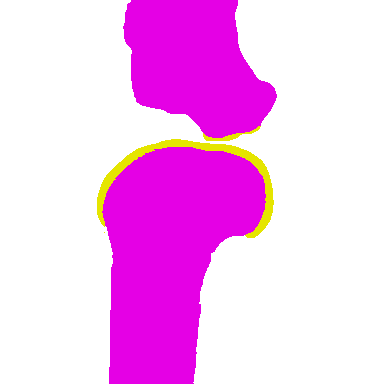
\includegraphics[width=\linewidth]{original_label_registration_1.png}
    \caption{Σταθερή απεικόνιση}
    \end{subfigure}
    \begin{subfigure}[t]{0.4\linewidth}
    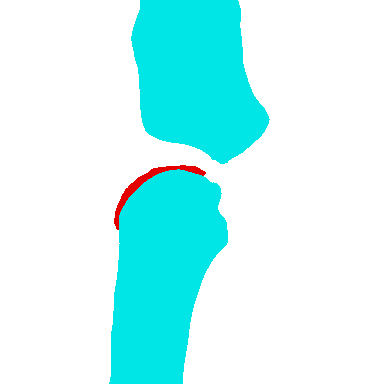
\includegraphics[width=\linewidth]{moving_label_before_registration_1.png}
    \caption{Κινούμενη απεικόνιση}
    \end{subfigure}

    \begin{subfigure}[t]{0.4\linewidth}
    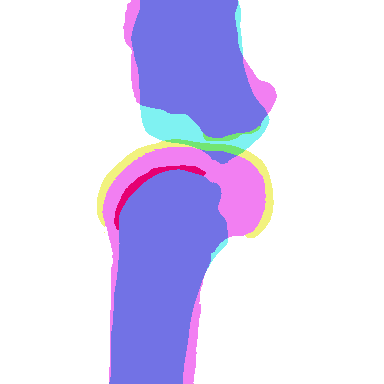
\includegraphics[width=\linewidth]{combination_label_before_registration_1.png}
    \caption{Σταθερή και κινούμενη}
    \end{subfigure}

    \caption{Τομή απεικονίσεων σταθερής και κινούμενης απεικόνισης και του
             συνδυασμού τους μετά την καταχώρηση.}
    \label{fig:registration_before:1}
\end{figure}

\begin{figure}[H]
    \centering

    \begin{subfigure}[t]{0.4\linewidth}
    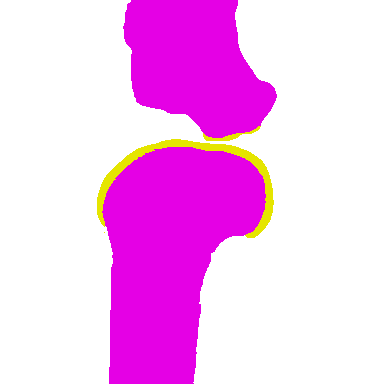
\includegraphics[width=\linewidth]{original_label_registration_1.png}
    \caption{Σταθερή απεικόνιση}
    \end{subfigure}
    \begin{subfigure}[t]{0.4\linewidth}
    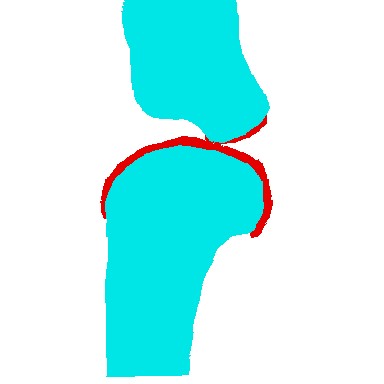
\includegraphics[width=\linewidth]{moving_label_after_registration_1.png}
    \caption{Κινούμενη απεικόνιση}
    \end{subfigure}

    \begin{subfigure}[t]{0.4\linewidth}
    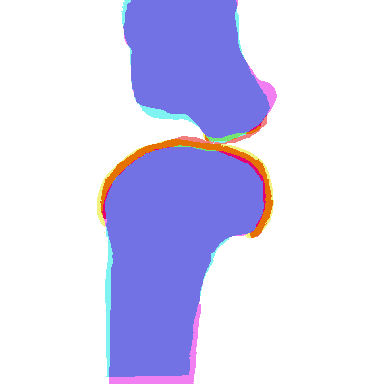
\includegraphics[width=\linewidth]{combination_label_after_registration_1.png}
    \caption{Σταθερή και κινούμενη}
    \end{subfigure}

    \caption{Τομή απεικονίσεων σταθερής και κινούμενης απεικόνισης και του
             συνδυασμού τους μετά την καταχώρηση.}
    \label{fig:registration_after:1}
\end{figure}

% 2
\begin{figure}[H]
    \centering

    \begin{subfigure}[t]{0.4\linewidth}
    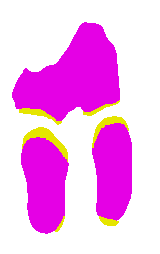
\includegraphics[width=\linewidth]{original_label_registration_2.png}
    \caption{Σταθερή απεικόνιση}
    \end{subfigure}
    \begin{subfigure}[t]{0.4\linewidth}
    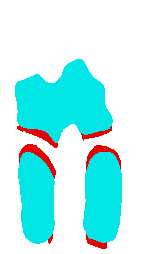
\includegraphics[width=\linewidth]{moving_label_before_registration_2.png}
    \caption{Κινούμενη απεικόνιση}
    \end{subfigure}

    \begin{subfigure}[t]{0.4\linewidth}
    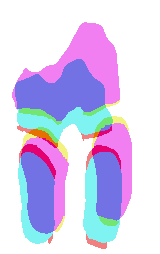
\includegraphics[width=\linewidth]{combination_label_before_registration_2.png}
    \caption{Σταθερή και κινούμενη}
    \end{subfigure}

    \caption{Τομή απεικονίσεων σταθερής και κινούμενης απεικόνισης και του
             συνδυασμού τους μετά την καταχώρηση.}
    \label{fig:registration_before:2}
\end{figure}

\begin{figure}[H]
    \centering

    \begin{subfigure}[t]{0.4\linewidth}
    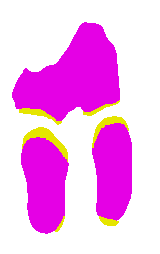
\includegraphics[width=\linewidth]{original_label_registration_2.png}
    \caption{Σταθερή απεικόνιση}
    \end{subfigure}
    \begin{subfigure}[t]{0.4\linewidth}
    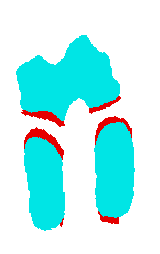
\includegraphics[width=\linewidth]{moving_label_after_registration_2.png}
    \caption{Κινούμενη απεικόνιση}
    \end{subfigure}

    \begin{subfigure}[t]{0.4\linewidth}
    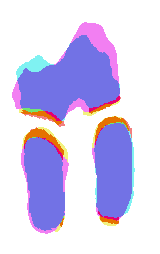
\includegraphics[width=\linewidth]{combination_label_after_registration_2.png}
    \caption{Σταθερή και κινούμενη}
    \end{subfigure}

    \caption{Τομή απεικονίσεων σταθερής και κινούμενης απεικόνισης και του
             συνδυασμού τους μετά την καταχώρηση.}
    \label{fig:registration_after:2}
\end{figure}

% 3
\begin{figure}[H]
    \centering

    \begin{subfigure}[t]{0.4\linewidth}
    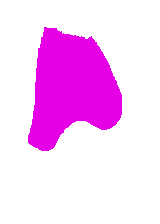
\includegraphics[width=\linewidth]{original_label_registration_3.png}
    \caption{Σταθερή απεικόνιση}
    \end{subfigure}
    \begin{subfigure}[t]{0.4\linewidth}
    
\includegraphics[width=\linewidth]{moving_label_before_registration_3.png}
    \caption{Κινούμενη απεικόνιση}
    \end{subfigure}

    \begin{subfigure}[t]{0.4\linewidth}
    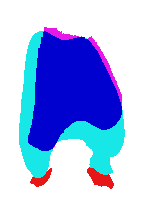
\includegraphics[width=\linewidth]{combination_label_before_registration_3.png}
    \caption{Σταθερή και κινούμενη}
    \end{subfigure}

    \caption{Τομή απεικονίσεων σταθερής και κινούμενης απεικόνισης και του
             συνδυασμού τους μετά την καταχώρηση.}
    \label{fig:registration_before:3}
\end{figure}

\begin{figure}[H]
    \centering

    \begin{subfigure}[t]{0.4\linewidth}
    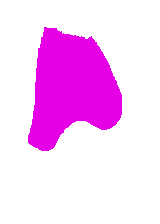
\includegraphics[width=\linewidth]{original_label_registration_3.png}
    \caption{Σταθερή απεικόνιση}
    \end{subfigure}
    \begin{subfigure}[t]{0.4\linewidth}
    
\includegraphics[width=\linewidth]{moving_label_after_registration_3.png}
    \caption{Κινούμενη απεικόνιση}
    \end{subfigure}

    \begin{subfigure}[t]{0.4\linewidth}
    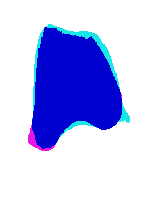
\includegraphics[width=\linewidth]{combination_label_after_registration_3.png}
    \caption{Σταθερή και κινούμενη}
    \end{subfigure}

    \caption{Τομή απεικονίσεων σταθερής και κινούμενης απεικόνισης και του
             συνδυασμού τους μετά την καταχώρηση.}
    \label{fig:registration_after:3}
\end{figure}


\subsection{Επιλογή ατλάντων}

Έπειτα από την καταχώρηση των ατλάντων επιλέγεται ένα υποσύνολο τους για να
χρησιμοποιηθεί στην κατάτμηση. Αυτό γίνεται ώστε να μειωθεί ο υπολογιστικός
χρόνος που απαιτείται. Ως μετρική για την επιλογή αυτή χρησιμοποιείται η μέση
διαφορά τετραγώνων των εικονοστοιχείων των απεικονίσεων που δεν ανήκουν στο
παρασκήνιο.  Συγκεκριμένα αν $I$ είναι η σταθερή απεικόνιση, $I_i$ και $L_i$ μία
κινούμενη απεικόνιση και οι ετικέτες της αντίστοιχα για τον $i$-οστό άτλαντα. Τα
στοιχεία της κινούμενης εικόνας που δεν ανήκουν στο παρασκήνιο είναι:

\begin{equation*}
    p_i = \{\bm{x}| \bm{x} \in L_i, L_i > 0 \}
\end{equation*}

Οι ετικέτες $L_i$ έχουν την τιμή $0$ για το παρασκήνιο και για τις υπόλοιπες
ακέραιους μεγαλύτερους του $0$. Έχοντας τα στοιχεία αυτά η μετρική ορίζεται ως:

\begin{equation} \label{mse_selection:1}
    mse_i = \frac {1} {\abs{p_i}} \sum_{\bm{x} \in p_i} ( I(\bm{x}) -
                I_i(\bm{x})  )^2
\end{equation}

Όπου $\abs{p_i}$ είναι ο αριθμός των στοιχείων που χρησιμοποιούνται για τον
υπολογισμό της μετρικής.

Έχοντας υπολογίσει την μετρική για όλους τους άτλαντες μέσω της
\eqref{mse_selection:1}, αν ο επιθυμητός αριθμός ατλάντων είναι $N$, τότε
επιλέγονται οι $N$ άτλαντες με την μικρότερη τιμή.


\subsection{Μέθοδοι κατάτμησης}

Για την κατάτμηση των απεικονίσεων χρησιμοποιήθηκαν τρεις μέθοδοι που έχουν
χρησιμοποιηθεί για την κατάτμηση απεικονίσεων μαγνητικής τομογραφίας του
εγκεφάλου \cite{Zhang:1} \cite{Tong:1} \cite{Coupe:1}.

\subsubsection{Αραιή μέθοδος βασισμένη σε τμήματα} \label{SPBM:1}

Η αραιή μέθοδος βασισμένη σε τμήματα (Sparse Patch-Based Method, SPBM) βασίζεται
στο \cite{Zhang:1}. Η μέθοδος αυτή ανοικοδομεί τα τμήματα γύρο από κάθε
εικονοστοιχείο της σταθερής απεικόνισης με αραιή γραμμική υπέρθεση των τμημάτων
των ατλάντων. Έπειτα χρησιμοποιεί τους συντελεστές της ανοικοδόμησης για να
εξαχθεί η δομή γειτνίασης γραφήματος και τα βάρη γραφήματος ταυτόχρονα, ώστε να
χρησιμοποιηθούν στο πλαίσιο συγχώνευσης κατηγοριών βασισμένο σε γράφους
(\ref{Graph-Based_Framework:1}).

Συγκεκριμένα έστω το ζεύγος $\{(I_i,L_i), i=1,...,n\}$ όπου $I_i$ είναι η
απεικόνιση ενός άτλαντα, $L_i$ ο χάρτης των κατηγοριών της αντίστοιχης
απεικόνισης και $n$ το σύνολο των ατλάντων. Για κάθε εικονοστοιχείο $\bm{x}$ της
σταθερής απεικόνισης $I$ και κάθε εικονοστοιχείο $\bm{y} \in N_i(\bm{x})$ σε
κάθε άτλαντα $I_i$, είναι επιθυμητό τα βάρη $w_i(\bm{x},\bm{y})$ να
βελτιστοποιηθούν βάση της αραιής αναπαράσταση. $N_i(\bm{x})$ είναι μία γειτονιά
εικονοστοιχείων γύρω από τον άτλαντα $I_i$. Επίσης τα βάρη $w_i(\bm{x},\bm{y})$
είναι οι συντελεστές ανοικοδόμησης.

Ακόμα, έστω $A^i_y \triangleq col(\{I_i(\bm{y'} | \bm{y'} \in
P_{I_i}(\bm{y})\})$ και $b_{\bm{x}} \triangleq col( \{ I(\bm{x'} | \bm{x'} \in
P_{I}(\bm{y})\})$ διανύσματα και $P_{I}(\bm{x})$, $P_{I_i}(\bm{y})$ τμήματα της
απεικόνισης $I$ και $I_i$ γύρο από τα εικονοστοιχεία $\bm{x}$ και $\bm{y}$
αντίστοιχα. Επίσης $col$ είναι ένας τελεστής που ευθυγραμμίζει όλα τα στοιχεία
ενός συνόλου σε ένα διάνυσμα στήλης. Ο συντελεστής ανοικοδόμησης
$w_i(\bm{x},\bm{y})$ υπολογίζεται από την παρακάτω συνάρτηση:

\begin{equation} \label{eq:SPBM:1}
    \argminB_{\{w_i(\bm{x},\bm{y})\}} { \frac{1} {2} \norm {\sum_{i=1}^{n}
    \sum_{\bm{y} \in N_i(\bm{x})} A_{\bm{y}}^i w_i(\bm{x},\bm{y}) -
    b_{\bm{x}}}_2^2 }
    + \lambda \sum_{i=1}^{n} \sum_{\bm{y} \in N_i(\bm{x})}
    \abs{w_i(\bm{x},\bm{y})}
\end{equation}

Με την συνάρτηση \eqref{eq:SPBM:1} επιθυμείτε η ανοικοδόμηση του διανύσματος
$b_{\bm{x}}$ της σταθερής εικόνας από το διάνυσμα $A^i_{\bm{y}}$ των ατλάντων. Ο
πρώτος όρος ελαχιστοποιεί το σφάλμα ανοικοδόμησης ενώ ο δεύτερος χρησιμοποιείται
ώστε να επιτευχθεί αραιή λύση. Η παράμετρος $\lambda$ χρησιμοποιείται για να
ελέγξει την συνεισφορά κάθε όρου και επομένως και το πόσο αραιό θα είναι το
αποτέλεσμα. Η συνάρτηση \eqref{eq:SPBM:1} μπορεί να ελαχιστοποιηθεί με τον
ελάχιστα απόλυτο τελεστή συρρίκνωσης και επιλογής (\ref{lasso:1}).

Έπειτα, αφού έχει υπολογιστεί ο συντελεστής ανοικοδόμησης $w_i(\bm{x},\bm{y})$, 
χρησιμοποιείται η εξίσωση \eqref{label_fusion:1} του πλαισίου συγχώνευσης
κατηγοριών, για να παραχθεί η ετικέτα $L(\bm{x})$ για το εικονοστοιχείο
$\bm{x}$.  Η διαδικασία του πλαισίου συγχώνευσης κατηγοριών επαναλαμβάνεται για
κάθε ετικέτα των δεδομένων εκτός του υποβάθρου. Η συνάρτηση αυτή επιστρέφει
τιμές στο διάστημα $[0,1]$. Αν όλες οι τιμές αυτές είναι μικρότερες του $0.5$,
τότε επιλέγεται για το εικονοστοιχείο $\bm{x}$ η ετικέτα του παρασκηνίου. Αλλιώς
επιλέγεται η ετικέτα με την μεγαλύτερη τιμή. Ολόκληρη η διαδικασία αυτή
επαναλαμβάνεται για κάθε εικονοστοιχείο $\bm{x} \in \Omega$ της σταθερής
απεικόνισης, όπου $\Omega$ ο χώρος των απεικονίσεων.


\subsubsection{Ταξινόμηση αραιής αναπαράστασης} \label{SRC:1}

Η μέθοδος ταξινόμησης αραιής αναπαράστασης (Sparse Representation
Classification, SRC) βασίζεται στο \cite{Tong:1} και χρησιμοποιεί μία βιβλιοθήκη
πρότυπων τμημάτων ως προκαθορισμένο λεξικό. Όπως και στην προηγούμενη μέθοδο, τα
τμήματα γύρο από κάθε εικονοστοιχείο της σταθερής απεικόνισης ανοικοδομούνται με
αραιή γραμμική υπέρθεση των τμημάτων των ατλάντων (δημιουργία βιβλιοθήκης
πρότυπων τμημάτων). Η κατηγορία-ετικέτα του εικονοστοιχείου προς ταξινόμηση
καθορίζεται από το σφάλμα ανοικοδόμησης για κάθε κατηγορία.

Τα βήματα για τη δημιουργία της βιβλιοθήκης πρότυπων τμημάτων είναι τα ίδια με
την αραιή μέθοδος βασισμένη σε τμήματα (\ref{SPBM:1}). Οι συντελεστές
$w_i(\bm{x},\bm{y})$ ανοικοδόμησης υπολογίζονται μέσω της \eqref{eq:SPBM:1}.

Για ευκολία η συνάρτηση \eqref{eq:SPBM:1} μπορεί να γραφτεί ως:

\begin{equation} \label{eq:SPBM:2}
    \argminB_{w_{\bm{x}}} { \frac{1} {2} \norm { A w_{\bm{x}} - b_{\bm{x}} }_2^2
              + \lambda \norm{w_{\bm{x}}}_1 }
\end{equation}

Όπου $w_{\bm{x}} \triangleq col( w_i( \bm{x}, \bm{y}) | \bm{y} \in N_i( \bm{x}),
i \in {{1,...,n}})$ και \\
$A \triangleq row( {{A_{\bm{y}}^i | \bm{y} \in N_i(\bm{x}), i \in {{1,...,n}}
}})$. Ο τελεστής $row$ ευθυγραμμίζει όλα τα διανύσματα κατά γραμμές, οπότε το
$A$ είναι πίνακας.

Έχοντας υπολογίσει τους συντελεστές ανοικοδόμησης (το διάνυσμα $w_{\bm{x}}$ στην
συνάρτηση \eqref{eq:SPBM:2}) μέσω του ελάχιστα απόλυτου τελεστή συρρίκνωσης και
επιλογής (\ref{lasso:1}), το σφάλμα ανοικοδόμησης για κάθε κλάση ορίζεται ως:

\begin{equation} 
    r_j(b_{\bm{x}}) = \norm{ b_{\bm{x}} - A^j w_{\bm{x}}^j }
\end{equation}

Όπου $A^j$ και $w_{\bm{x}}^j$ είναι τα $A$ και $w_{\bm{x}}$ αντίστοιχα που
σχετίζονται με την ετικέτα $j$. Δηλαδή τα στοιχεία των $A$ και $w_{\bm{x}}$ που
δεν ανήκουν στην κατηγορία-ετικέτα $j$ έχουν την τιμή $0$ ή με άλλα λόγια δεν
συνεισφέρουν στον υπολογισμό του σφάλματος ανοικοδόμησης.

Τέλος, η τελική ετικέτα $v$ του εικονοστοιχείου προς ταξινόμηση ορίζεται ως:

\begin{equation*} 
    v = \argminB_{j} { \left( r_j(b_{\bm{x}}) \right) } \text{ , } j = 0,...,C
\end{equation*}

Όπου $C$ είναι ο μεγαλύτερος αριθμός ετικέτας. Η διαδικασία αυτή επαναλαμβάνεται
για κάθε εικονοστοιχείο $\bm{x} \in \Omega$ της σταθερής απεικόνισης, όπου
$\Omega$ ο χώρος των απεικονίσεων.


\subsubsection{Κατάτμηση βασισμένη σε τμήματα με τη χρήση πληροφορίας από
ειδικούς}

Η κατάτμηση βασισμένη σε τμήματα με τη χρήση πληροφορίας από ειδικούς
(Patch-Based Segmentation using Expert Priors, PBSEP) βασίζεται στο
\cite{Coupe:1}. Η μέθοδος αυτή αρχικά επιλέγει τα τμήματα των ατλάντων, γύρο από
το εικονοστοιχείο προς κατάτμηση, που ξεπερνούν ένα επίπεδο ομοιότητας σε σχέση
με το τμήματα της σταθερής απεικόνισης, γύρο από το εικονοστοιχείο προς
κατάτμηση, βάση απλών στατιστικών, όπως φωτεινότητα και αντίθεση. Έπειτα,
συγκρίνει τα τμήματα αυτά. Με την σύγκριση αυτή εξάγει μία μετρική ομοιότητας
των τμημάτων, ώστε να χρησιμοποιηθούν στο πλαίσιο συγχώνευσης κατηγοριών
βασισμένο σε γράφους (\ref{Graph-Based_Framework:1}).

Για την μετρική της ομοιότητας χρησιμοποιούνται οι όροι της φωτεινότητας και της
αντίθεσης του δείκτη δομικής ομοιότητας (\ref{SSIM:1}). Οι σταθερές της εξίσωσης
\eqref{eq:SSIM:1} είναι $\alpha = 1, \beta = 1, \gamma = 0$. Οπότε η μετρική
ορίζεται ως:

\begin{equation} \label{eq:ss:1}
    ss = \frac {2 \mu_i \mu_{s,j}} {\mu_i^2 + \mu_{s,j}^2} 
         \frac {2 \sigma_i \sigma_{s,j}} {\sigma_i^2 + \sigma_{s,j}^2}
\end{equation}

Όπου $\mu_i$ και $\sigma_i$ είναι η μέση τιμή και η τυπική απόκλιση αντίστοιχα
του τμήματος γύρο από το εικονοστοιχείο προς κατάτμηση. Επίσης, $\mu_{s,j}$ και
$\sigma_{s,j}$ είναι η μέση τιμή και η τυπική απόκλιση του τμήματος γύρο από το
εικονοστοιχείο $j$ του άτλαντα $s$.

Η επιλογή τμημάτων και η μετρική ομοιότητας ορίζονται από την εξίσωση:

\begin{equation} \label{eq:w_PBSEP:1}
    w(x_i, x_{s,j}) = 
    \begin{cases}
        exp\left( \frac {- \norm{P(x_i) - P(x_{s,j})}_2^2 } {h} \right)
            & \text{if } ss > th\\
        0   & \text{otherwise}
    \end{cases}
\end{equation}

Όπου $P(x_i)$ αναπαριστά ένα κυβικό τμήμα γύρο από το εικονοστοιχείο $x_i$. Τα
$x_i$ και $x_{s,j}$ είναι εικονοστοιχεία της σταθερής εικόνας στη θέση $i$ και
του άτλαντα $s$ στη θέση $j$ αντίστοιχα. Τα τμήματα που επιλέγονται έχουν τιμή
για την μετρική ομοιότητας της εξίσωσης \eqref{eq:ss:1} μεγαλύτερη της σταθεράς
$th$. Η παράμετρος απόσβεσης $h$ ορίζει την συνεισφορά των τμημάτων και ορίζεται
ως:

\begin{equation*} 
    h = \argminB_{x_{x,j}} \norm{P(x_i) - P(x_{s,j})}_2 + \epsilon
\end{equation*}

Το $\epsilon$ χρησιμοποιείται για υπολογιστική σταθερότητα της εξίσωσης
\eqref{eq:w_PBSEP:1} και είναι μία μικρή σταθερά.

Έπειτα, αφού έχει αφού έχει γίνει η επιλογή τμημάτων και έχουν υπολογιστεί τα
βάρη $w(x_i, x_{s,j})$ για $j \in N(x_i)$, όπου $N(x_i)$ αναπαριστά ένα κυβικό
τμήμα γύρο από το εικονοστοιχείο $x_i$, χρησιμοποιείται η εξίσωση
\eqref{label_fusion:1} του πλαισίου συγχώνευσης κατηγοριών για να παραχθεί η
ετικέτα $L(x_i)$ για το εικονοστοιχείο $x_i$. Αν όλα τα βάρη $w(x_i, x_{s,j})$
έχουν τιμή $0$, τότε επιλέγεται η ετικέτα του παρασκηνίου αυθαίρετα.
Διαφορετικά, η διαδικασία του πλαισίου συγχώνευσης κατηγοριών επαναλαμβάνεται
για κάθε ετικέτα των δεδομένων εκτός του υποβάθρου. Η συνάρτηση αυτή επιστρέφει
τιμές στο διάστημα $[0,1]$. Αν όλες οι τιμές αυτές είναι μικρότερες του $0.5$,
τότε επιλέγεται για το εικονοστοιχείο $x_i$ η ετικέτα του παρασκηνίου. Αλλιώς
επιλέγεται η ετικέτα με την μεγαλύτερη τιμή. Ολόκληρη η διαδικασία αυτή
επαναλαμβάνεται για κάθε εικονοστοιχείο $x_i \in \Omega$ της σταθερής
απεικόνισης, όπου $\Omega$ ο χώρος των απεικονίσεων.


\section{Πειράματα και αποτελέσματα}

\subsection{Τρόπος αξιολόγησης και σύγκρισης}

Για τις μεθόδους που προτάθηκαν στο προηγούμενο κεφάλαιο αρχικά, θα επιλεγούν οι
καλύτερες παράμετροι τους και έπειτα θα συγκριθούν μεταξύ τους. Τα δεδομένα που
θα χρησιμοποιηθούν για την παραπάνω διαδικασία παρουσιάστηκαν στο \ref{data:1}.
Επίσης ως μετρική του αποτελέσματος χρησιμοποιείται ο συντελεστής ομοιότητας
Dice (\ref{Dice:1}) που ορίζεται από την εξίσωση \eqref{eq:Dice:1}. Η μετρική
αυτή υπολογίζεται για κάθε ετικέτα των δεδομένων.

Επίσης, για κάθε πείραμα χρησιμοποιήθηκε η διασταυρωμένη επικύρωση αφήνω ένα έξω
(\ref{leave_one_out:1}). Η επιλογή αυτή έγινε ούτως ώστε να αξιολογηθεί η
δυνατότητα του μοντέλου να πραγματοποιεί σωστές προβλέψεις για δεδομένα που δεν
χρησιμοποιήθηκαν για την εκπαίδευση του.

\subsection{Λεπτομέρειες υλοποίησης}

Η υλοποίηση των μεθόδων έγινε στις γλώσσες προγραμματισμού \emph{Python 3} και
\emph{Cython}. Συγκεκριμένα, για την διαχείριση και επεξεργασία των
απεικονίσεων χρησιμοποιήθηκε το εργαλείο \emph{Simple ITK}. Για την καταχώριση
των απεικονίσεων χρησιμοποιήθηκε το εργαλείο \emph{Simple Elastix}. Οι μέθοδοι
κατάτμησης υλοποιήθηκαν σε \emph{Cython} για λόγους υπολογιστικής ταχύτητας.
Τέλος, το εργαλείο \emph{SPAMS} χρησιμοποιήθηκε για την επίλυση του ελάχιστα
απόλυτου τελεστή συρρίκνωσης και επιλογής (\ref{lasso:1}).

\subsection{Επιλογή παραμέτρων}

Οι παράμετροι που είναι κοινοί για όλες τις μεθόδους είναι:

\begin{enumerate}
    \item Ο αριθμός των ατλάντων που χρησιμοποιείται στην κατάτμηση.
    \item Το τμήμα αναζήτησης στους άτλαντες.
    \item Το τμήμα γύρο από κάθε εικονοστοιχείο προς κατάτμηση. Θα μπορούσε να
          χαρακτηριστεί και ως τμήμα χαρακτηριστικών.
\end{enumerate}

Ακόμα, η αραιή μέθοδος βασισμένη σε τμήματα (\ref{SPBM:1}) και η μέθοδος
ταξινόμησης αραιής αναπαράστασης (\ref{SRC:1}) έχουν την παράμετρο $\lambda$ του
ελάχιστα απόλυτου τελεστή συρρίκνωσης και επιλογής.

\subsubsection{Παράμετρος $\lambda$ του ελάχιστα απόλυτου τελεστή συρρίκνωσης
και επιλογής}

Αρχικά, επιλέγεται η καλύτερη τιμή της παραμέτρου $\lambda$ του ελάχιστα
απόλυτου τελεστή συρρίκνωσης και επιλογής. Η παράμετρος αυτή ελέγχει την
συνεισφορά του σφάλματος ανοικοδόμησης σε σχέση με τον όρο της πρώτης νόρμας που
χρησιμοποιείται ώστε να επιτευχθεί αραιή λύση.

\paragraphLine{Αραιή μέθοδος βασισμένη σε τμήματα}

Στην αραιή μέθοδο βασισμένη σε τμήματα η παράμετρος αυτή υπάρχει στην εξίσωση
\eqref{eq:SPBM:1}. Οι τιμές των υπόλοιπων παραμέτρων παρουσιάζονται στον
\autoref{table:lambda:1}.

\begin{table}[h!]
    \centering
    \begin{tabular}{|c|c|} 
        \hline
        Αριθμός ατλάντων & 4 \\ 
        \hline
        Τμήμα αναζήτησης & [5,5,5] \\ 
        \hline
        Τμήμα χαρακτηριστικών & [3,3,3] \\ 
        \hline
    \end{tabular}
    \caption{Παράμετροι που παραμένουν σταθεροί για την επιλογή της παραμέτρου
             $\lambda$.}
    \label{table:lambda:1}
\end{table}

Στα \autoref{fig:SPBM:lambda:1}, \autoref{fig:SPBM:lambda:2} και
\autoref{fig:SPBM:lambda:3} παρουσιάζονται οι τιμές του συντελεστή ομοιότητας
Dice για τις τιμές της παραμέτρου $\lambda$ που χρησιμοποιήθηκαν. Από τα
\autoref{fig:SPBM:lambda:1} και \autoref{fig:SPBM:lambda:2} παρατηρείται ότι
δεν υπάρχει μεγάλη διαφορά ανάμεσα στις τιμές του συντελεστή. Στο
\autoref{fig:SPBM:lambda:3} για τιμή $\lambda = 0.01$ παρατηρείται η μεγαλύτερη
τιμή του συντελεστή. Για το λόγο αυτό επιλέχτηκε η τιμή $\lambda = 0.01$.

\begin{figure}[H]
    \centering
    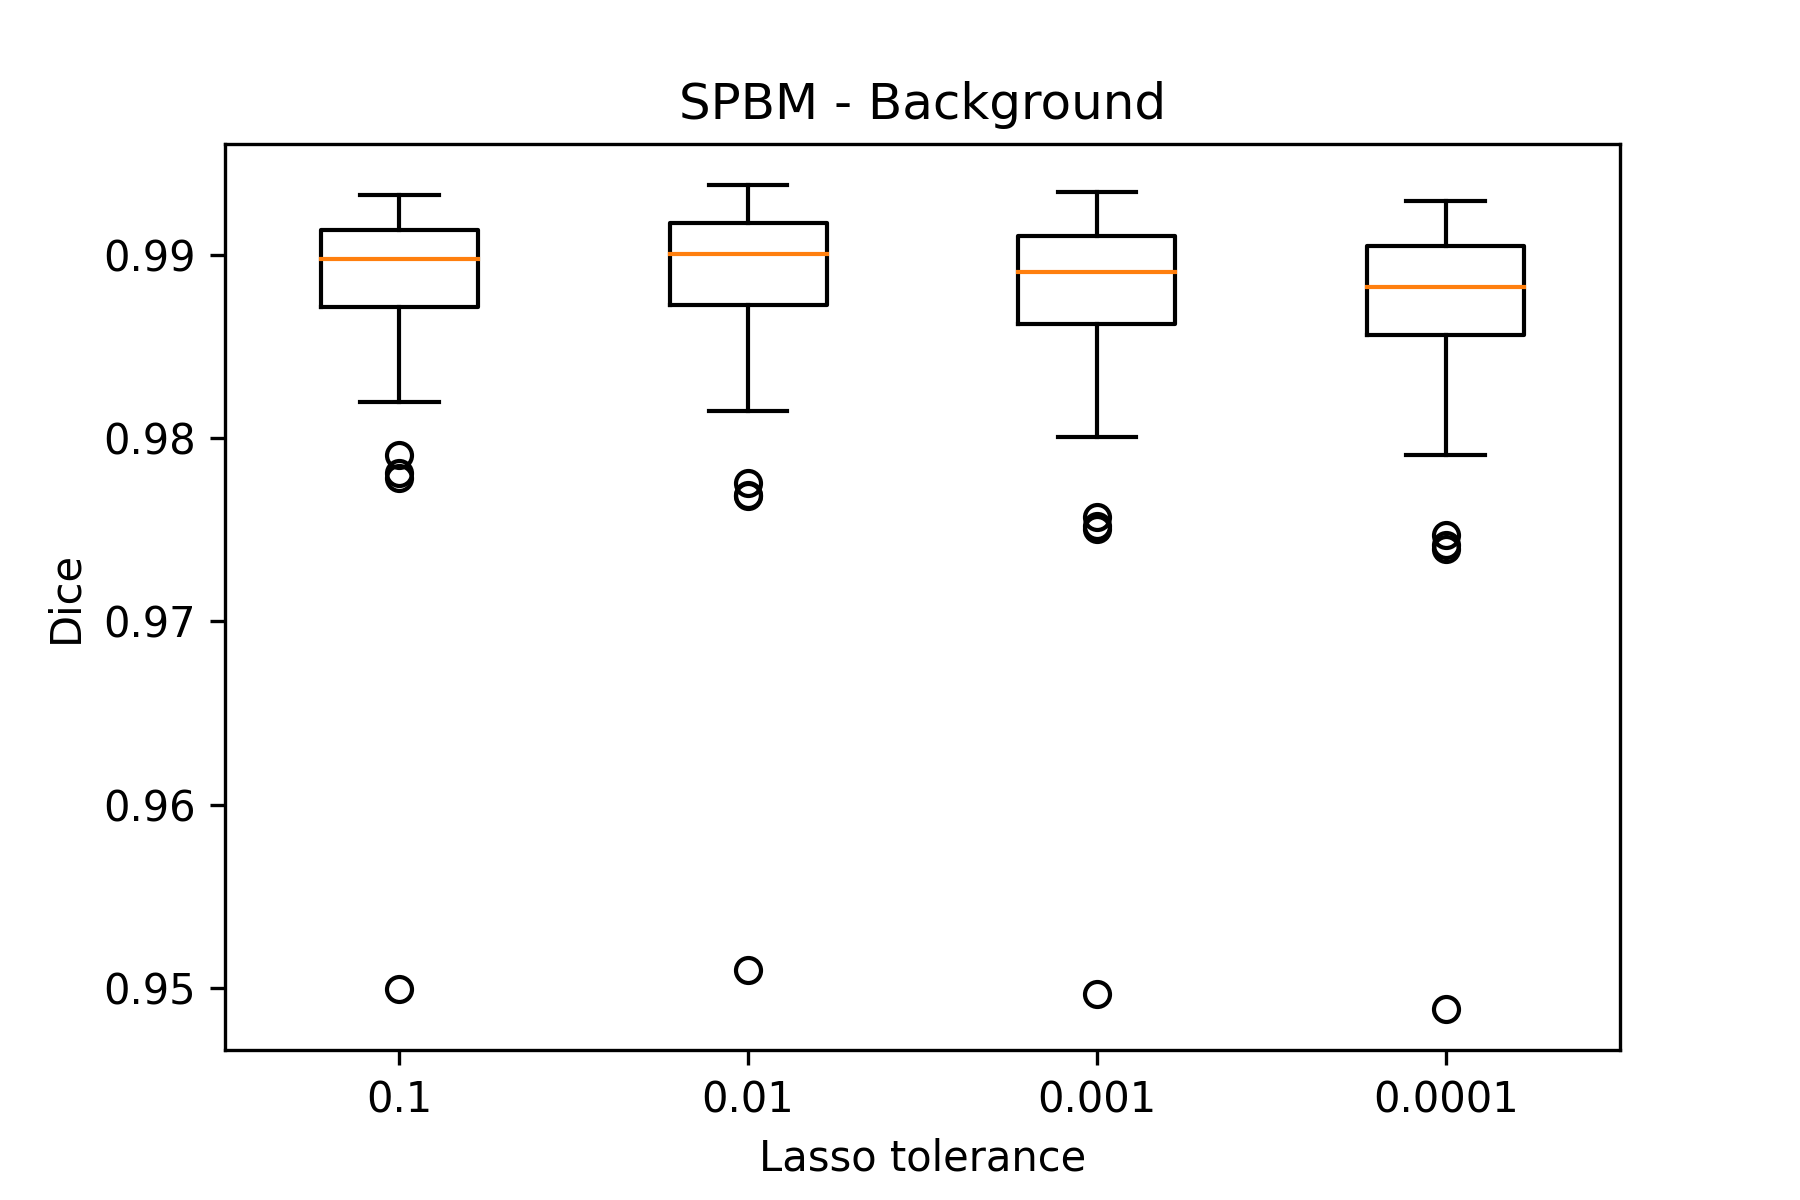
\includegraphics[width=0.85\linewidth]{SPBM_Lasso_tolerance_Background_plot.png}
    \caption{Μεταβολή της παραμέτρου $\lambda$ της αραιής μεθόδου βασισμένης σε
             τμήματα για την ετικέτα του παρασκηνίου.}
    \label{fig:SPBM:lambda:1}
\end{figure}

\begin{figure}[H]
    \centering
    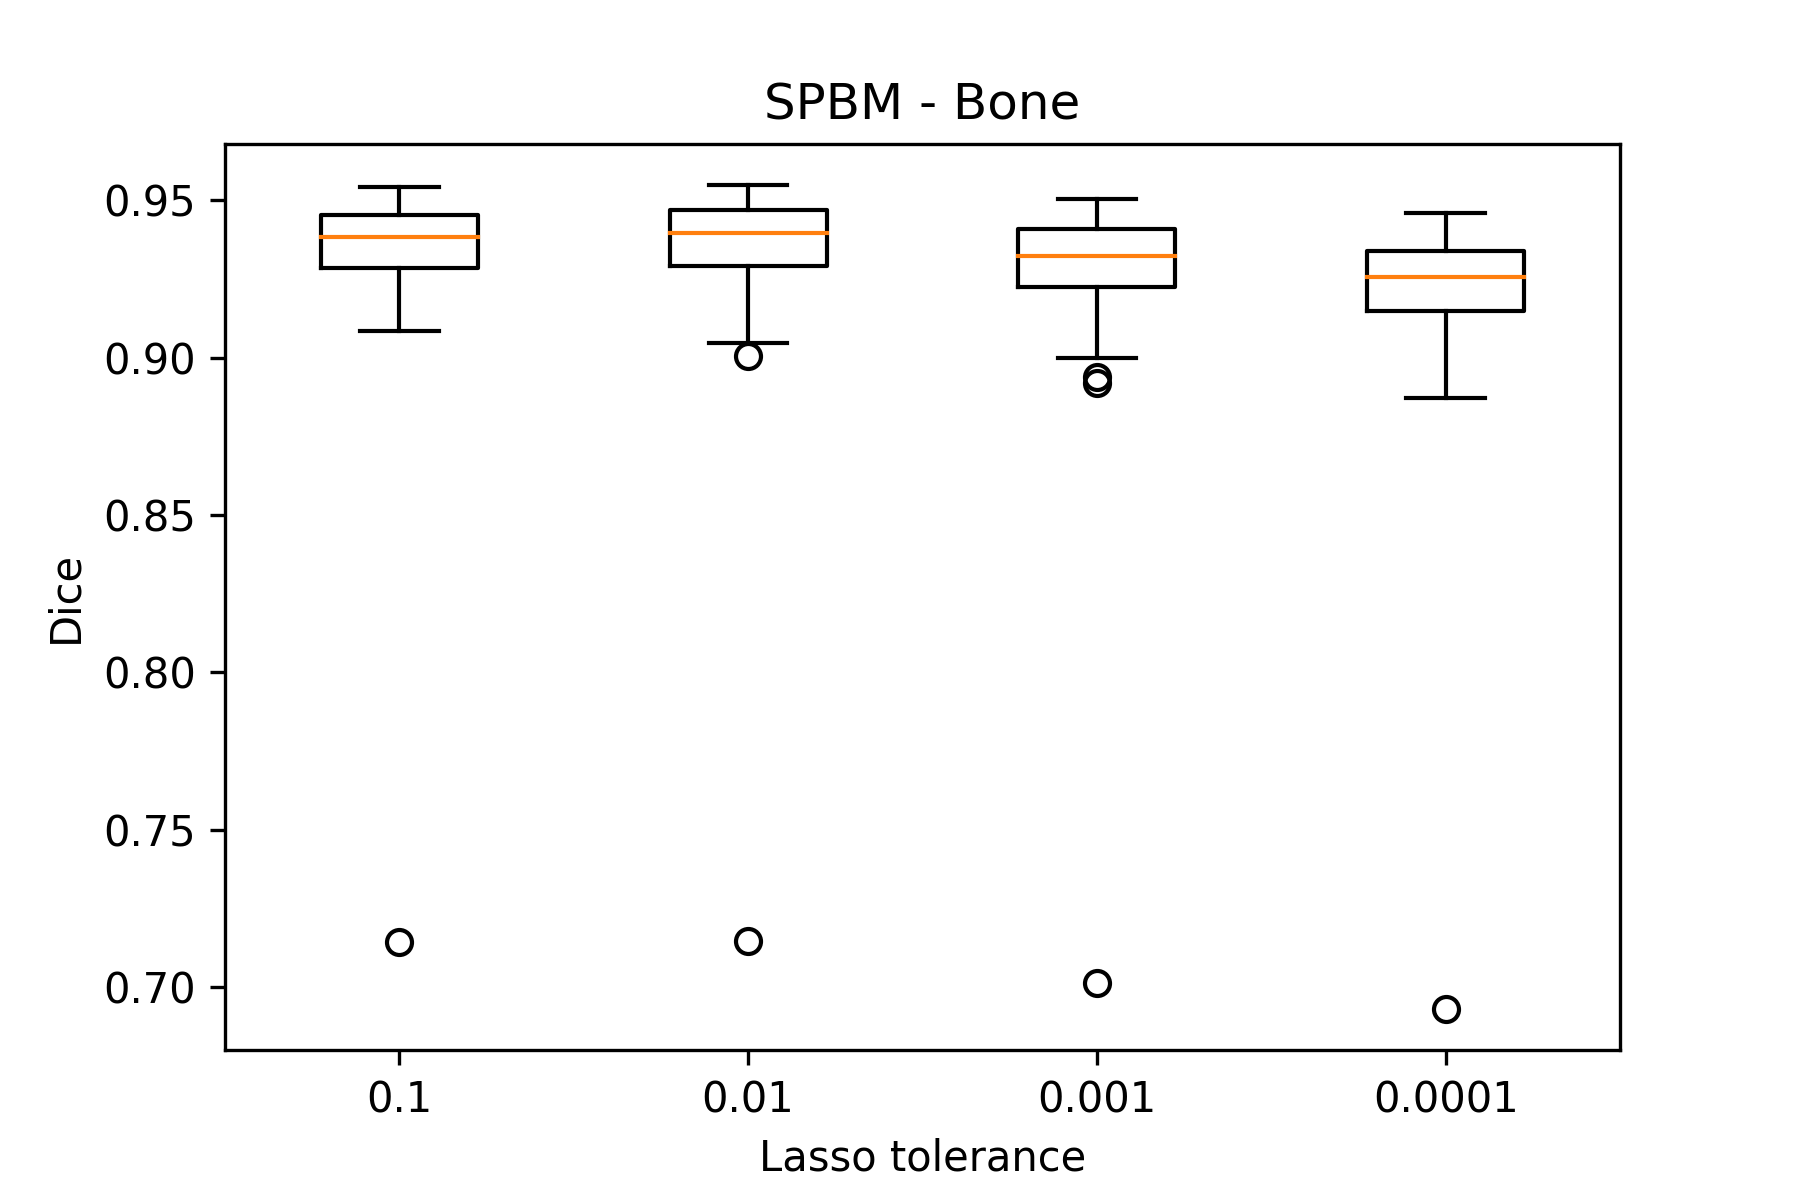
\includegraphics[width=0.85\linewidth]{SPBM_Lasso_tolerance_Bone_plot.png}
    \caption{Μεταβολή της παραμέτρου $\lambda$ της αραιής μεθόδου βασισμένης σε
             τμήματα για την ετικέτα των οστών.}
    \label{fig:SPBM:lambda:2}
\end{figure}

\begin{figure}[H]
    \centering
    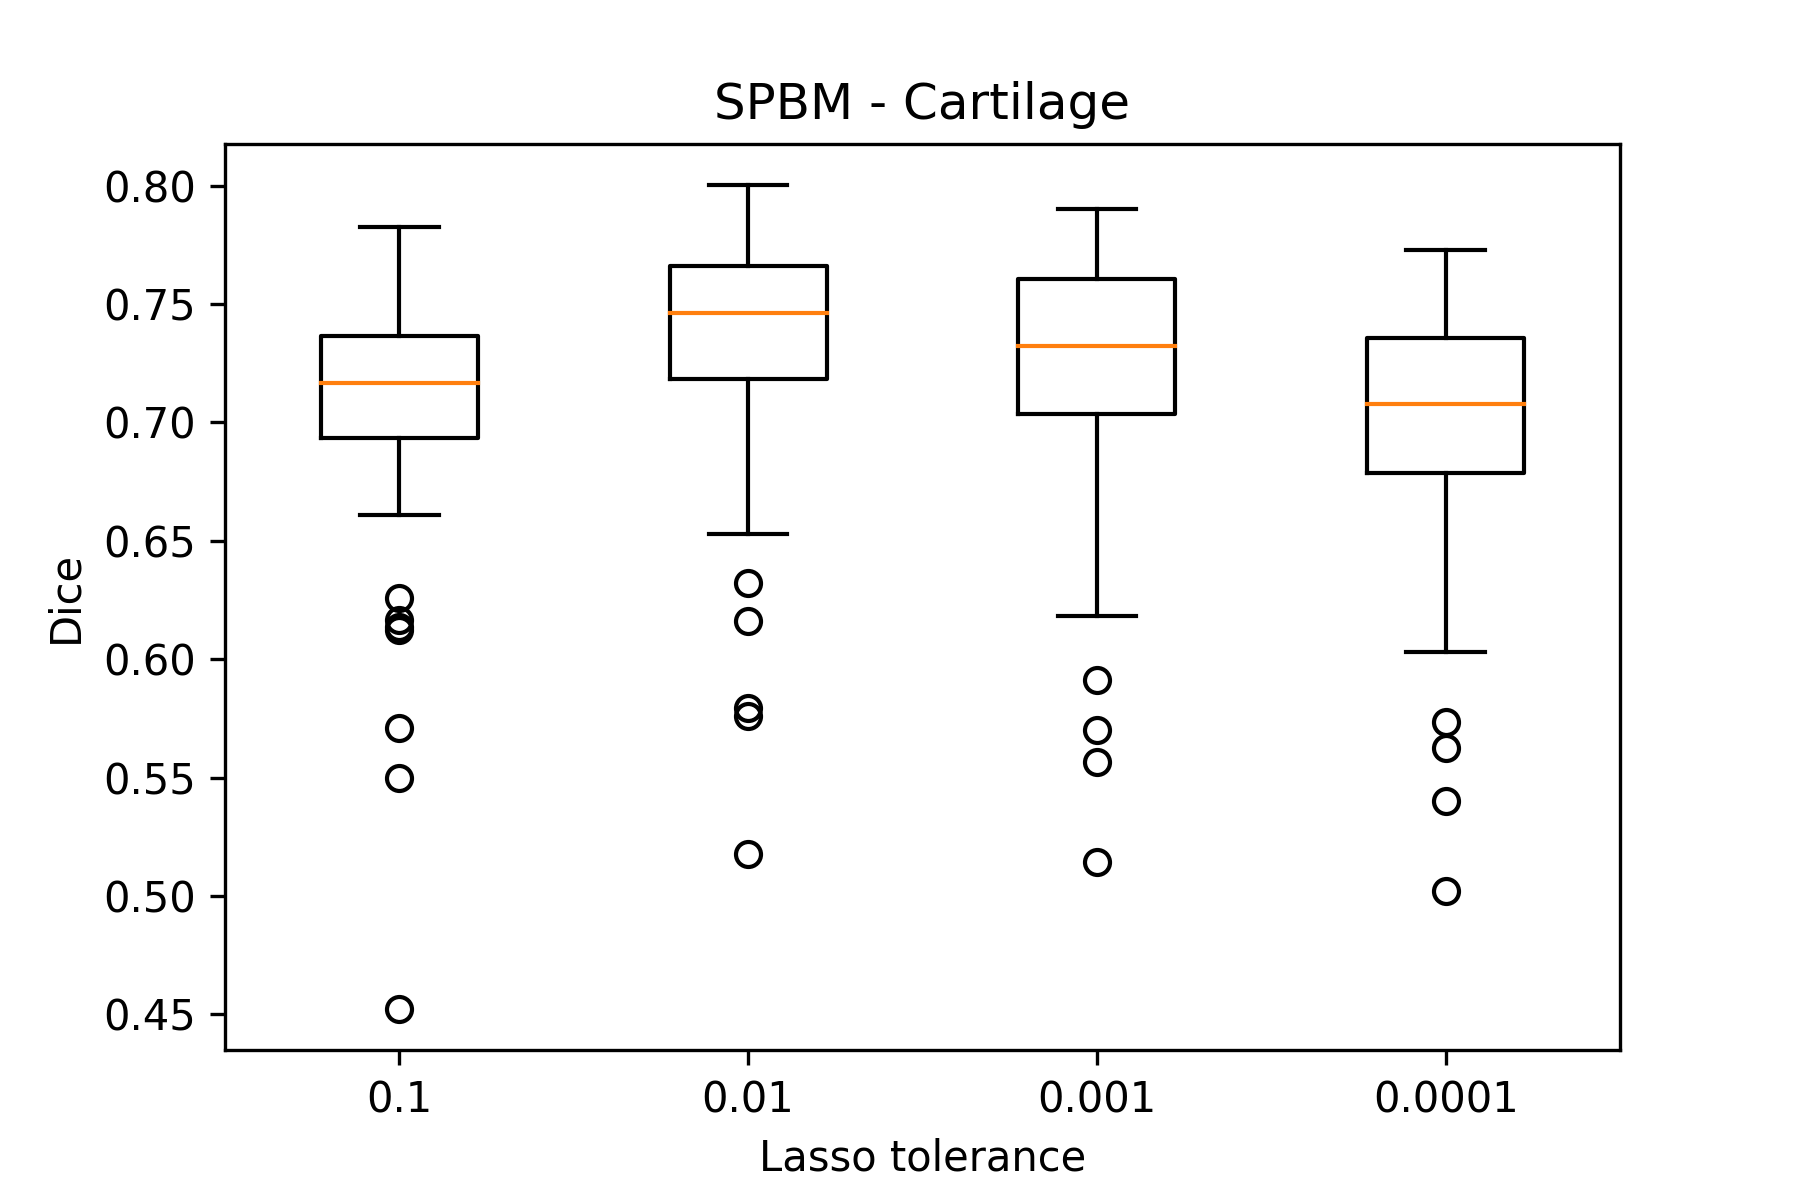
\includegraphics[width=0.85\linewidth]{SPBM_Lasso_tolerance_Cartilage_plot.png}
    \caption{Μεταβολή της παραμέτρου $\lambda$ της αραιής μεθόδου βασισμένης σε
             τμήματα για την ετικέτα των χόνδρων.}
    \label{fig:SPBM:lambda:3}
\end{figure}

\paragraphLine{Ταξινόμηση αραιής αναπαράστασης}

Στην μέθοδο ταξινόμησης αραιής αναπαράστασης η παράμετρος αυτή υπάρχει στην
εξίσωση \eqref{eq:SPBM:2}. Οι τιμές των υπόλοιπων παραμέτρων παρουσιάζονται στον
\autoref{table:lambda:1} και είναι ίδιες με αυτές που χρησιμοποιήθηκαν στην
αραιή μέθοδο βασισμένη σε τμήματα.

Στα \autoref{fig:SRC:lambda:1}, \autoref{fig:SRC:lambda:2} και
\autoref{fig:SRC:lambda:3} παρουσιάζονται οι τιμές του συντελεστή ομοιότητας
Dice για τις τιμές της παραμέτρου $\lambda$ που χρησιμοποιήθηκαν. Παρατηρείται,
ιδίως στο \autoref{fig:SRC:lambda:3}, ότι για μικρότερες τιμές της παραμέτρου
$\lambda$ το αποτέλεσμα είναι καλύτερο. Γι᾽ αυτό το λόγο, επιλέχτηκε η τιμή
$\lambda = 0.1$.

\begin{figure}[H]
    \centering
    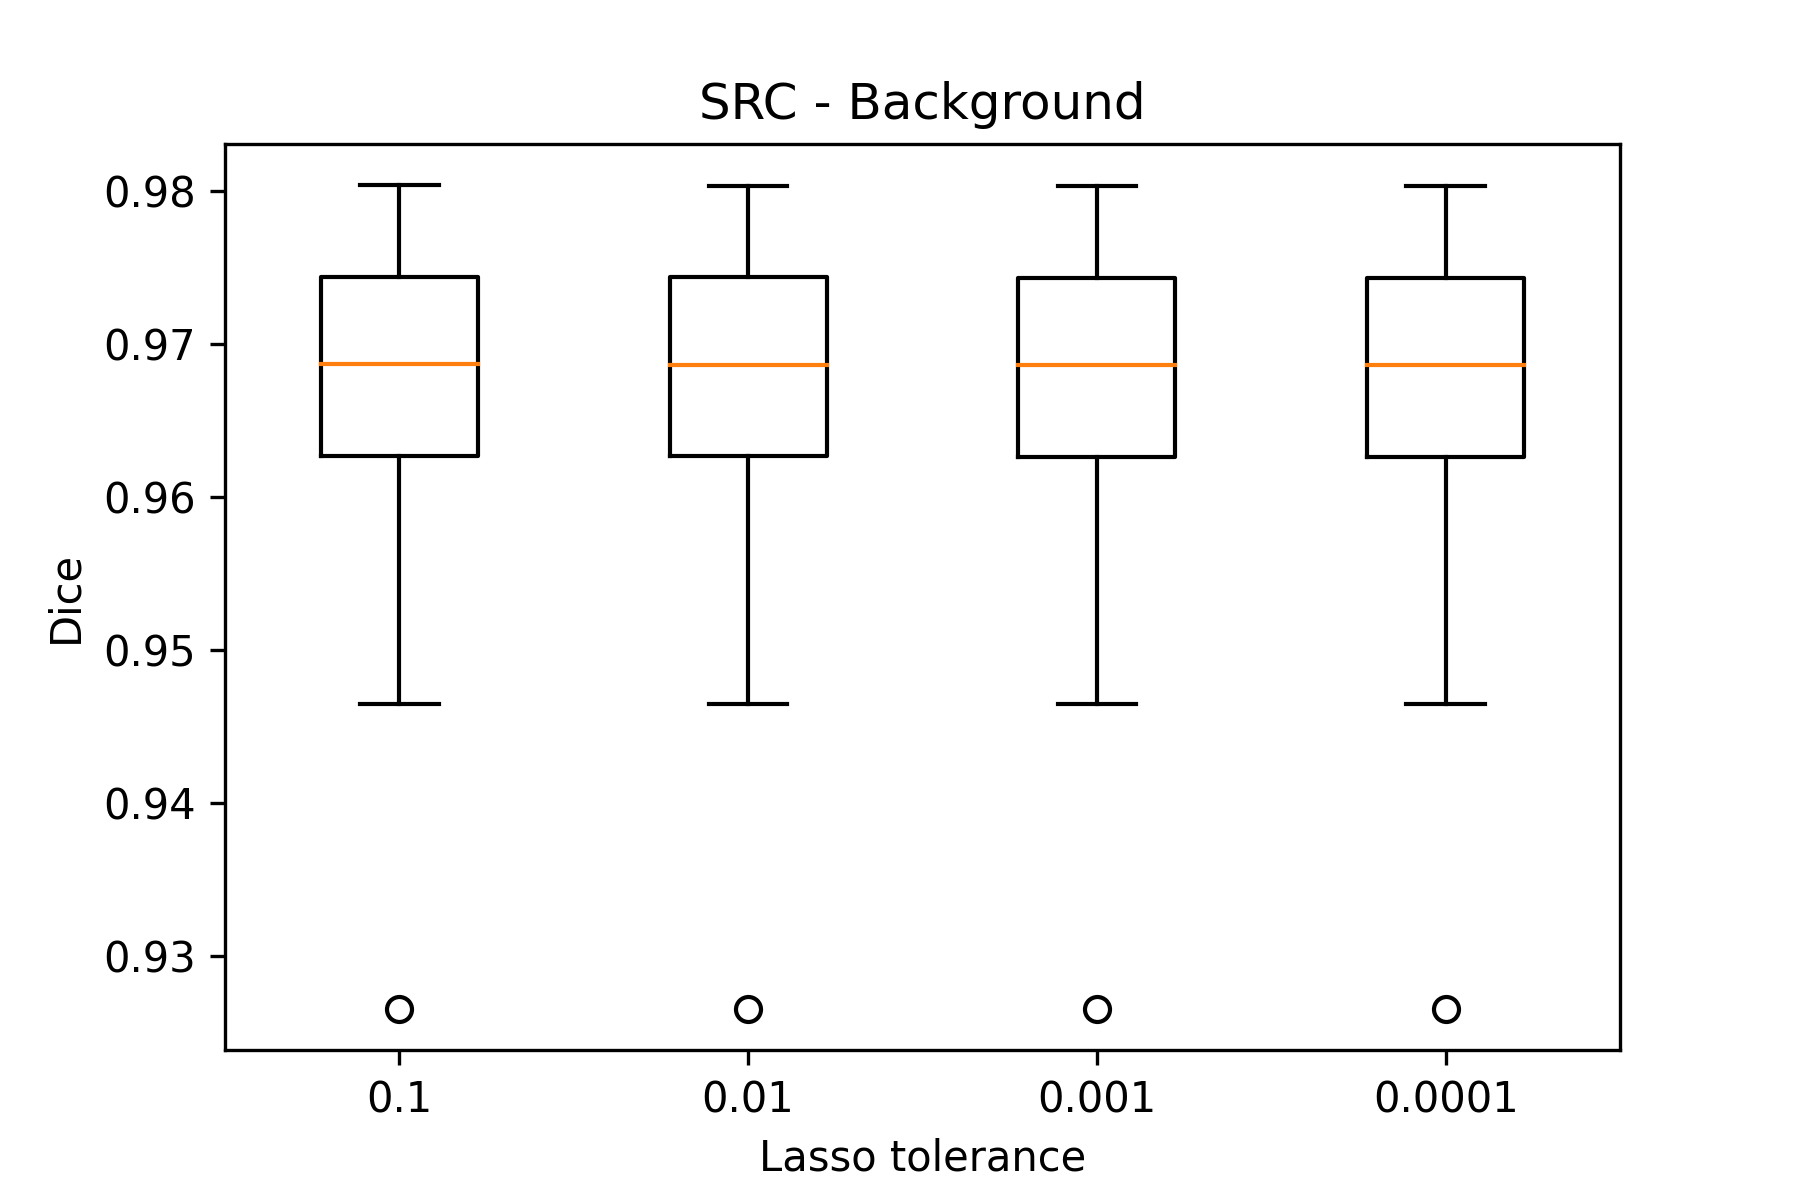
\includegraphics[width=0.85\linewidth]{SRC_Lasso_tolerance_Background_plot.png}
    \caption{Μεταβολή της παραμέτρου $\lambda$ της μεθόδου ταξινόμησης αραιής
             αναπαράστασης για την ετικέτα του παρασκηνίου.}
    \label{fig:SRC:lambda:1}
\end{figure}

\begin{figure}[H]
    \centering
    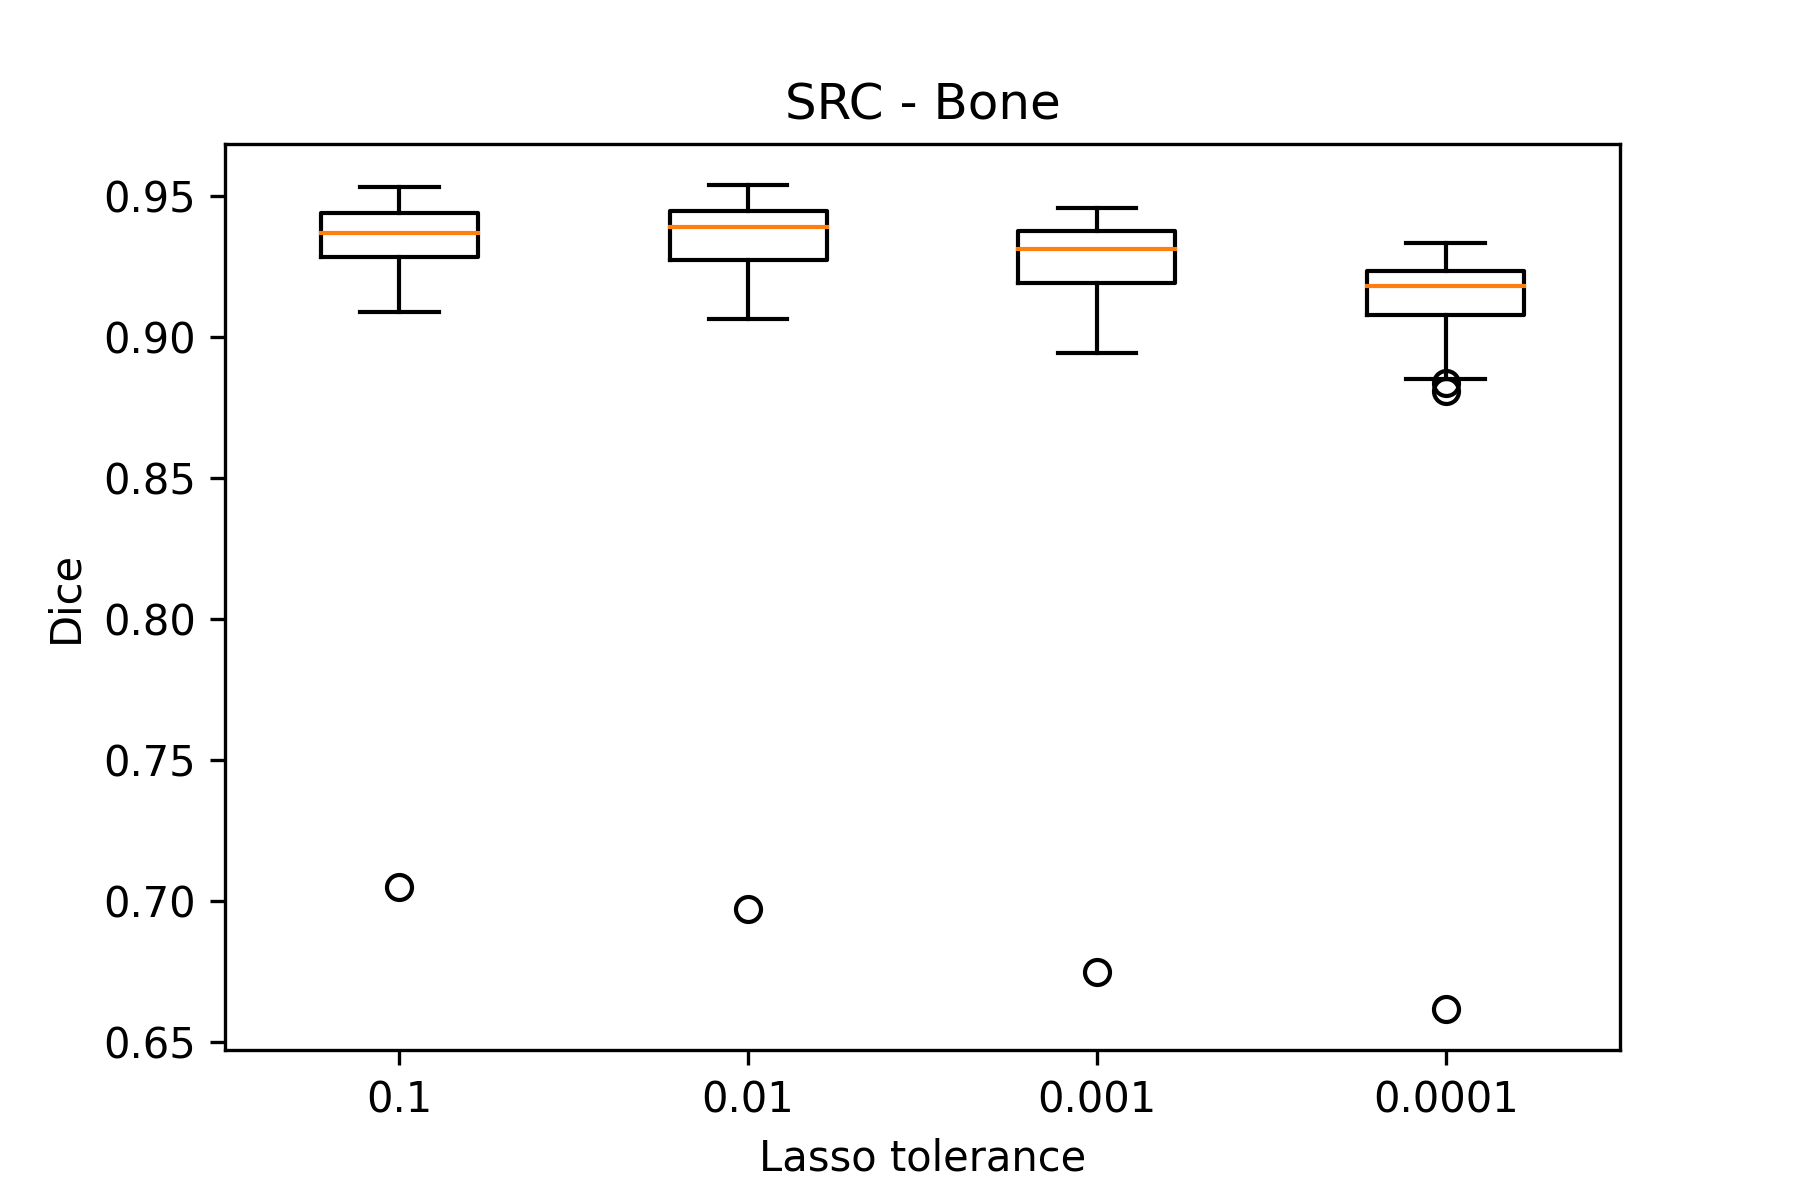
\includegraphics[width=0.85\linewidth]{SRC_Lasso_tolerance_Bone_plot.png}
    \caption{Μεταβολή της παραμέτρου $\lambda$ της μεθόδου ταξινόμησης αραιής
             αναπαράστασης για την ετικέτα των οστών.}
    \label{fig:SRC:lambda:2}
\end{figure}

\begin{figure}[H]
    \centering
    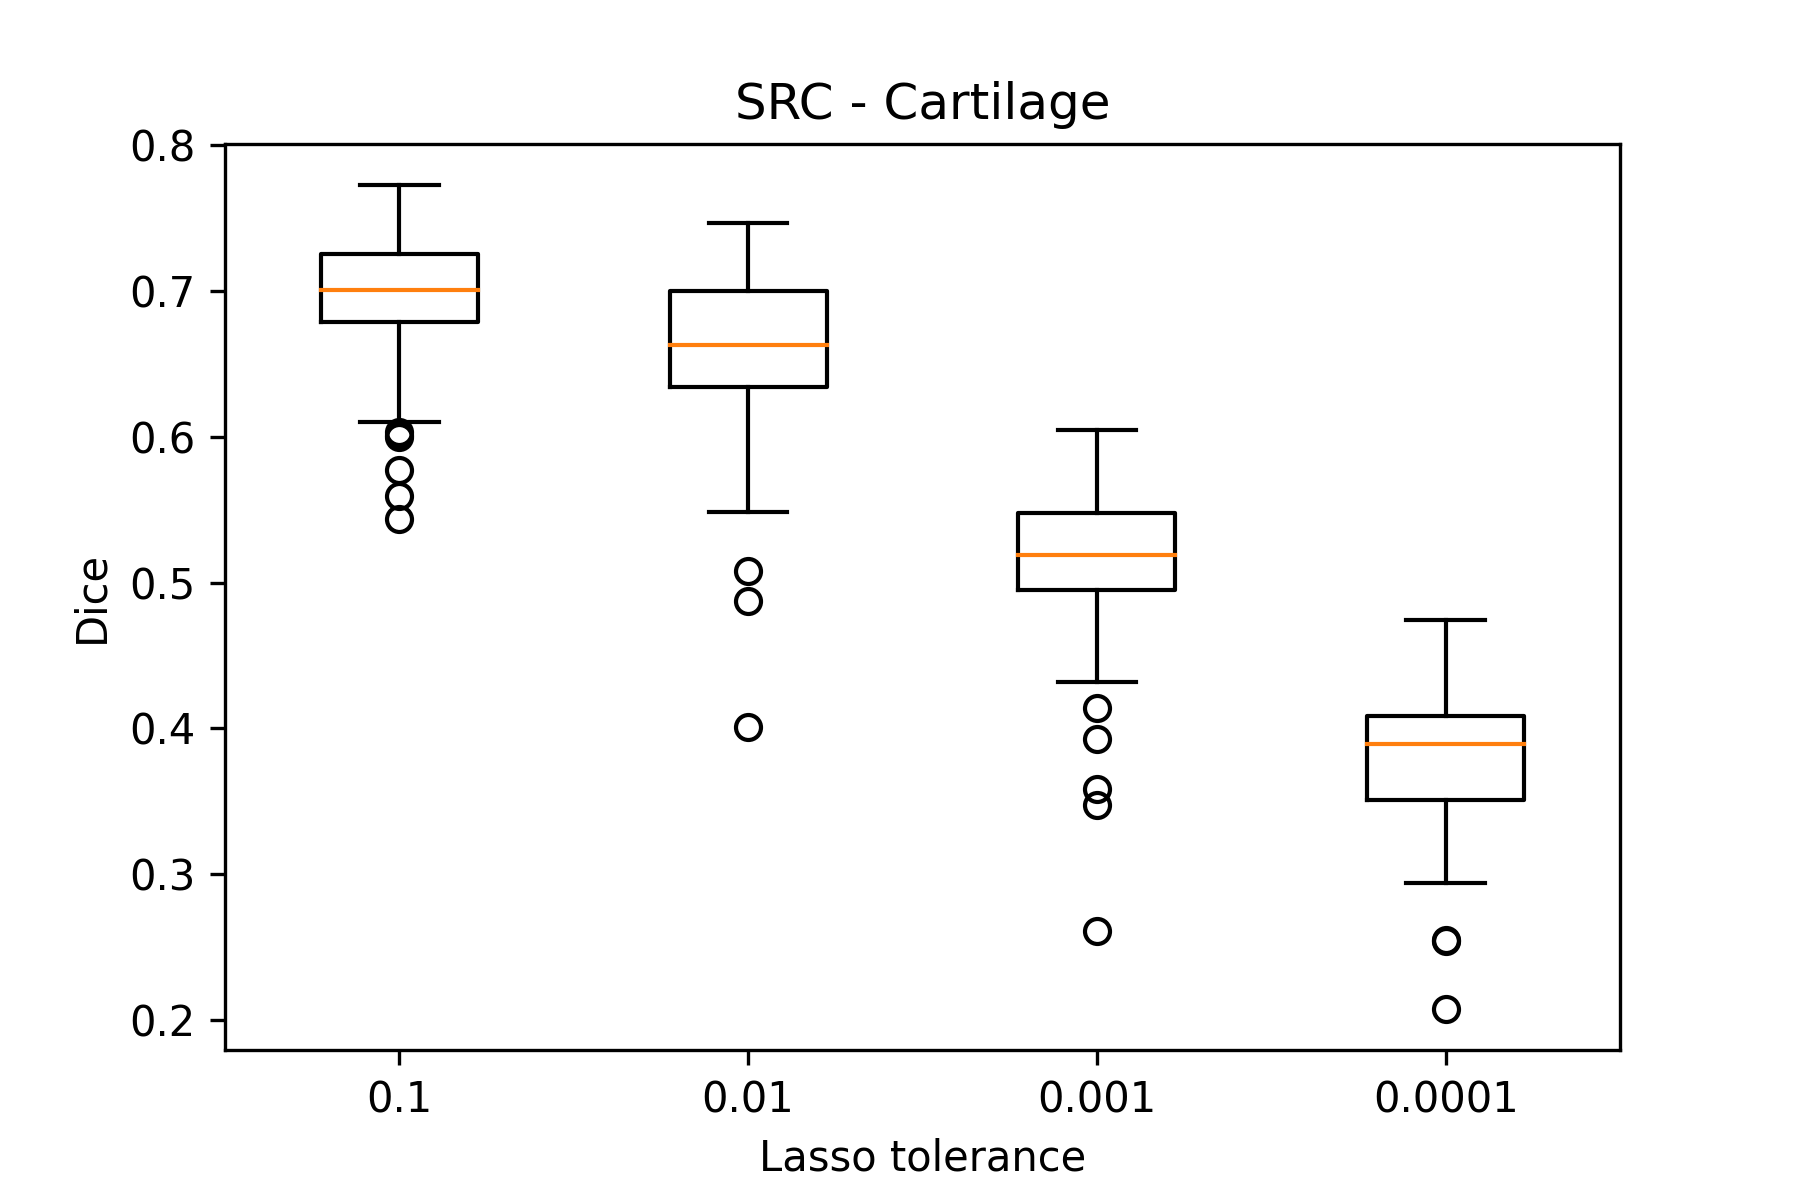
\includegraphics[width=0.85\linewidth]{SRC_Lasso_tolerance_Cartilage_plot.png}
    \caption{Μεταβολή της παραμέτρου $\lambda$ της μεθόδου ταξινόμησης αραιής
             αναπαράστασης για την ετικέτα των χόνδρων.}
    \label{fig:SRC:lambda:3}
\end{figure}


\subsubsection{Τμήμα αναζήτησης}

\paragraphLine{Αραιή μέθοδος βασισμένη σε τμήματα}

Τα πειράματα για την επιλογή του τμήματος αναζήτησης έγιναν με τις σταθερές
παραμέτρους που παρουσιάζονται στον \autoref{table:N:1}.

\begin{table}[h!]
    \centering
    \begin{tabular}{|c|c|} 
        \hline
        Παράμετρος $\lambda$ & 0.01 \\ 
        \hline
        Αριθμός ατλάντων & 4 \\ 
        \hline
        Τμήμα χαρακτηριστικών & [3,3,3] \\ 
        \hline
    \end{tabular}
    \caption{Παράμετροι που παραμένουν σταθεροί για την επιλογή του τμήματος
             αναζήτησης της αραιής μεθόδου βασισμένης σε τμήματα.}
    \label{table:N:1}
\end{table}

Στα \autoref{fig:SPBM:N:1}, \autoref{fig:SPBM:N:2} και \autoref{fig:SPBM:N:3}
παρουσιάζονται οι τιμές του συντελεστή ομοιότητας Dice για διάφορες τιμές του
τμήματος αναζήτησης. Παρατηρείται, κυρίως στο \autoref{fig:SPBM:N:3}, ότι για
μικρότερες τιμές του τμήματος το αποτέλεσμα είναι καλύτερο. Το γεγονός αυτό αυτό
δεν είναι αναμενόμενο αφού θα περίμενε κανείς, το μέγεθος του τμήματος
αναζήτησης και η ποιότητα του αποτελέσματος να είναι ανάλογα μεγέθη. Μία πιθανή
εξήγηση είναι ότι το αποτέλεσμα της καταχώρισης είναι αρκετά καλό ώστε, τμήματα
με κεντρικό εικονοστοιχείο μακριά από το εικονοστοιχείο προς καταχώρηση να είναι
ασυσχέτιστα με το εικονοστοιχείο αυτό, έτσι ώστε να θεωρούνται θόρυβος
και να έχουν μόνο αρνητική επίδραση στο αποτέλεσμα. Η εξήγηση αυτή είναι λάθος
διότι, όπως θα παρουσιαστεί παρακάτω, το φαινόμενο αυτό δεν παρατηρείται στη
κατάτμηση βασισμένη σε τμήματα με τη χρήση πληροφορίας από ειδικούς. Οπότε,
πιθανότατα αυτή η μέθοδος είναι πιο επιρρεπής στο θόρυβο. Για το λόγο αυτό
επιλέχτηκε η τιμή $[3,3,3]$ του τμήματος αναζήτησης.


\begin{figure}[H]
    \centering
    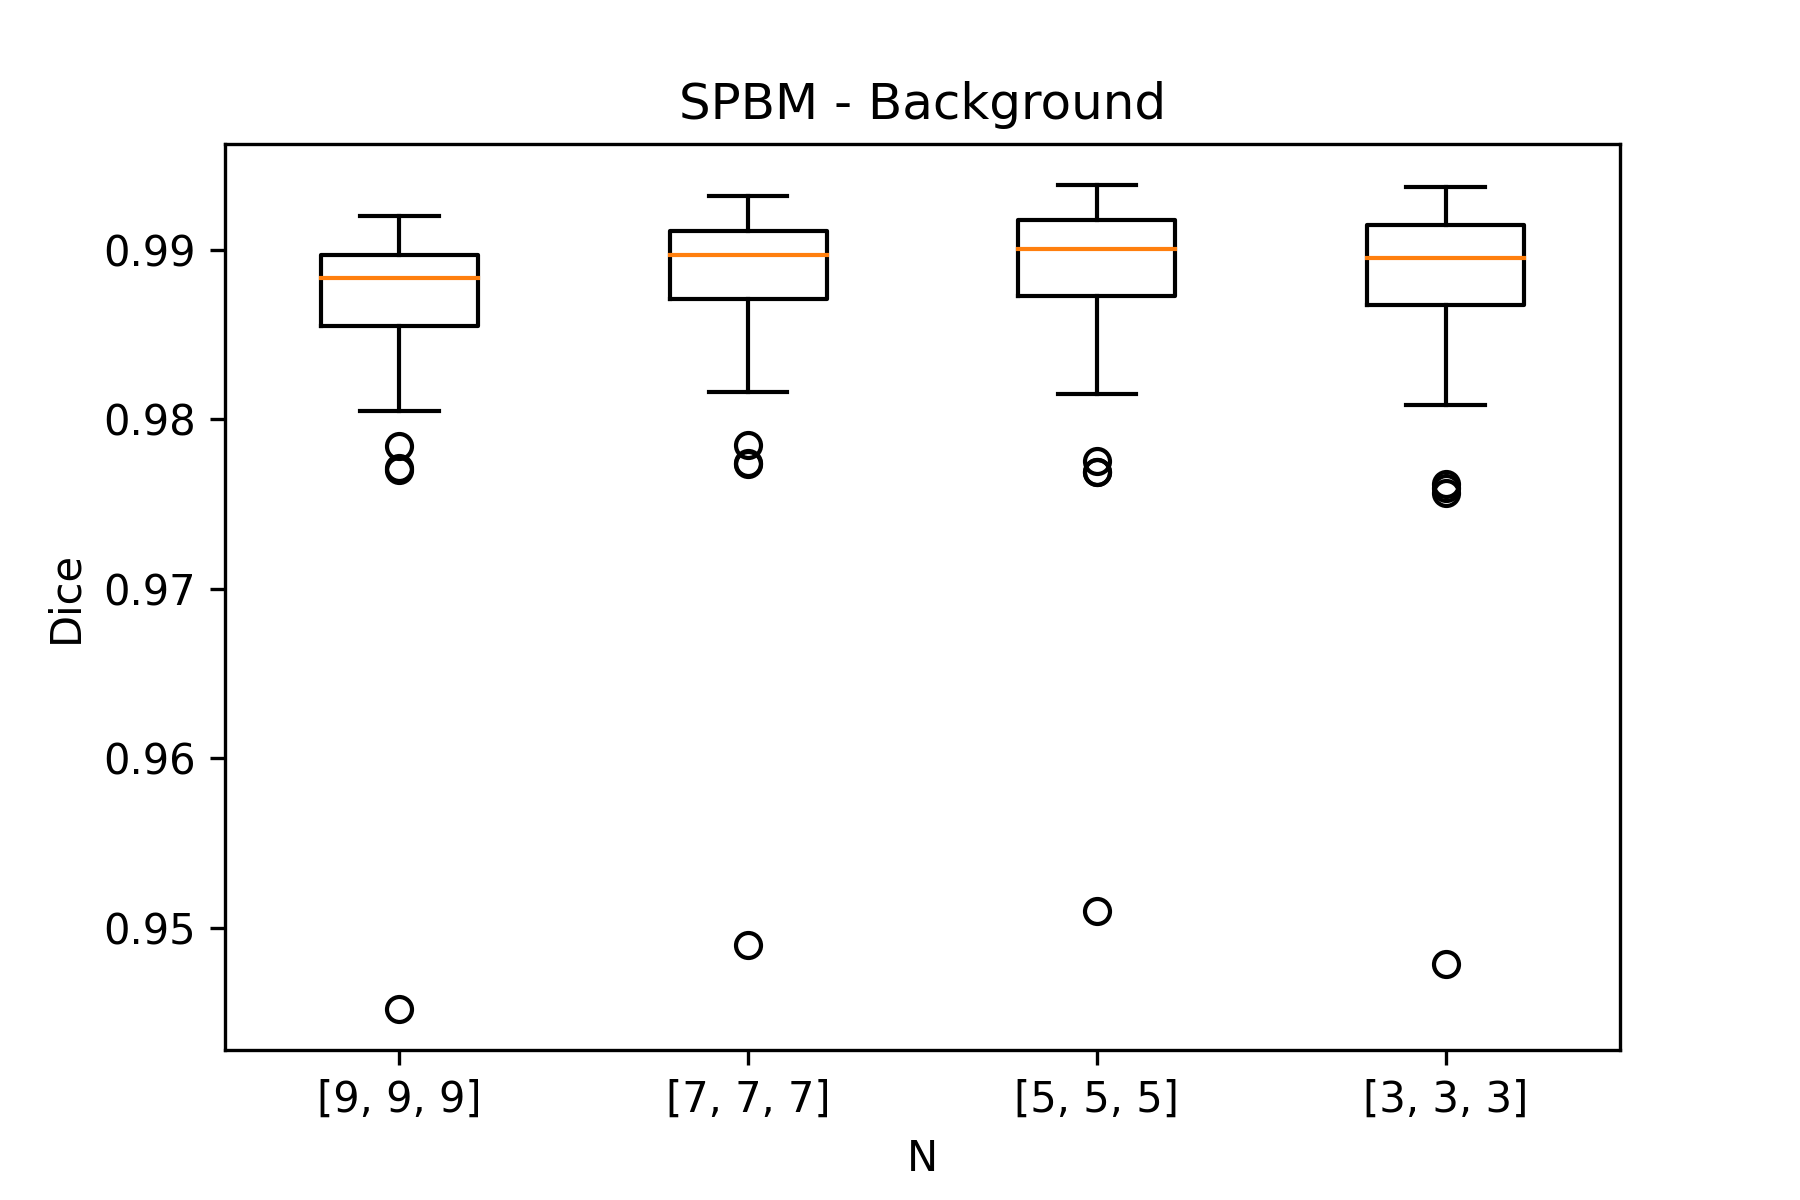
\includegraphics[width=0.85\linewidth]{SPBM_N_Background_plot.png}
    \caption{Μεταβολή του τμήματος αναζήτησης της αραιής μεθόδου βασισμένης σε
             τμήματα για την ετικέτα του παρασκηνίου.}
    \label{fig:SPBM:N:1}
\end{figure}

\begin{figure}[H]
    \centering
    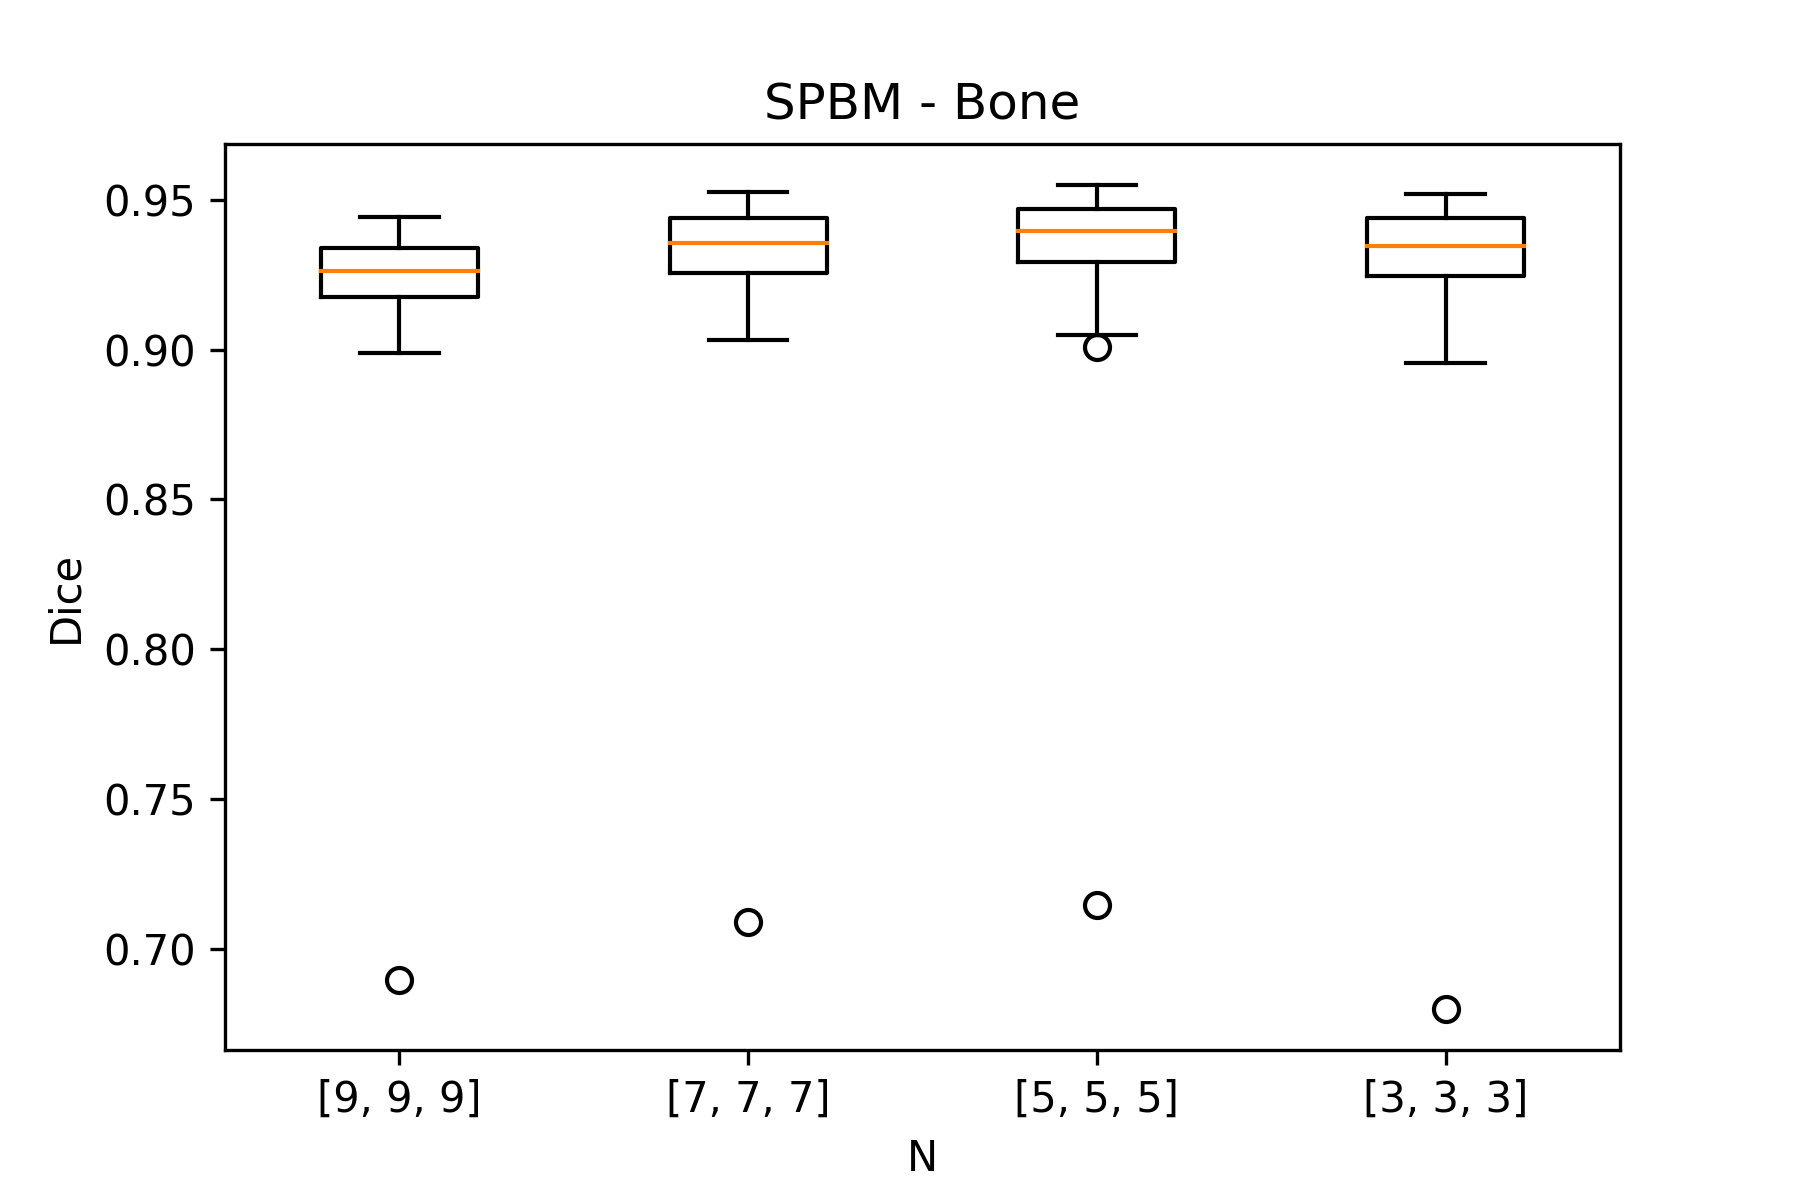
\includegraphics[width=0.85\linewidth]{SPBM_N_Bone_plot.png}
    \caption{Μεταβολή του τμήματος αναζήτησης της αραιής μεθόδου βασισμένης σε
             τμήματα για την ετικέτα των οστών.}
    \label{fig:SPBM:N:2}
\end{figure}

\begin{figure}[H]
    \centering
    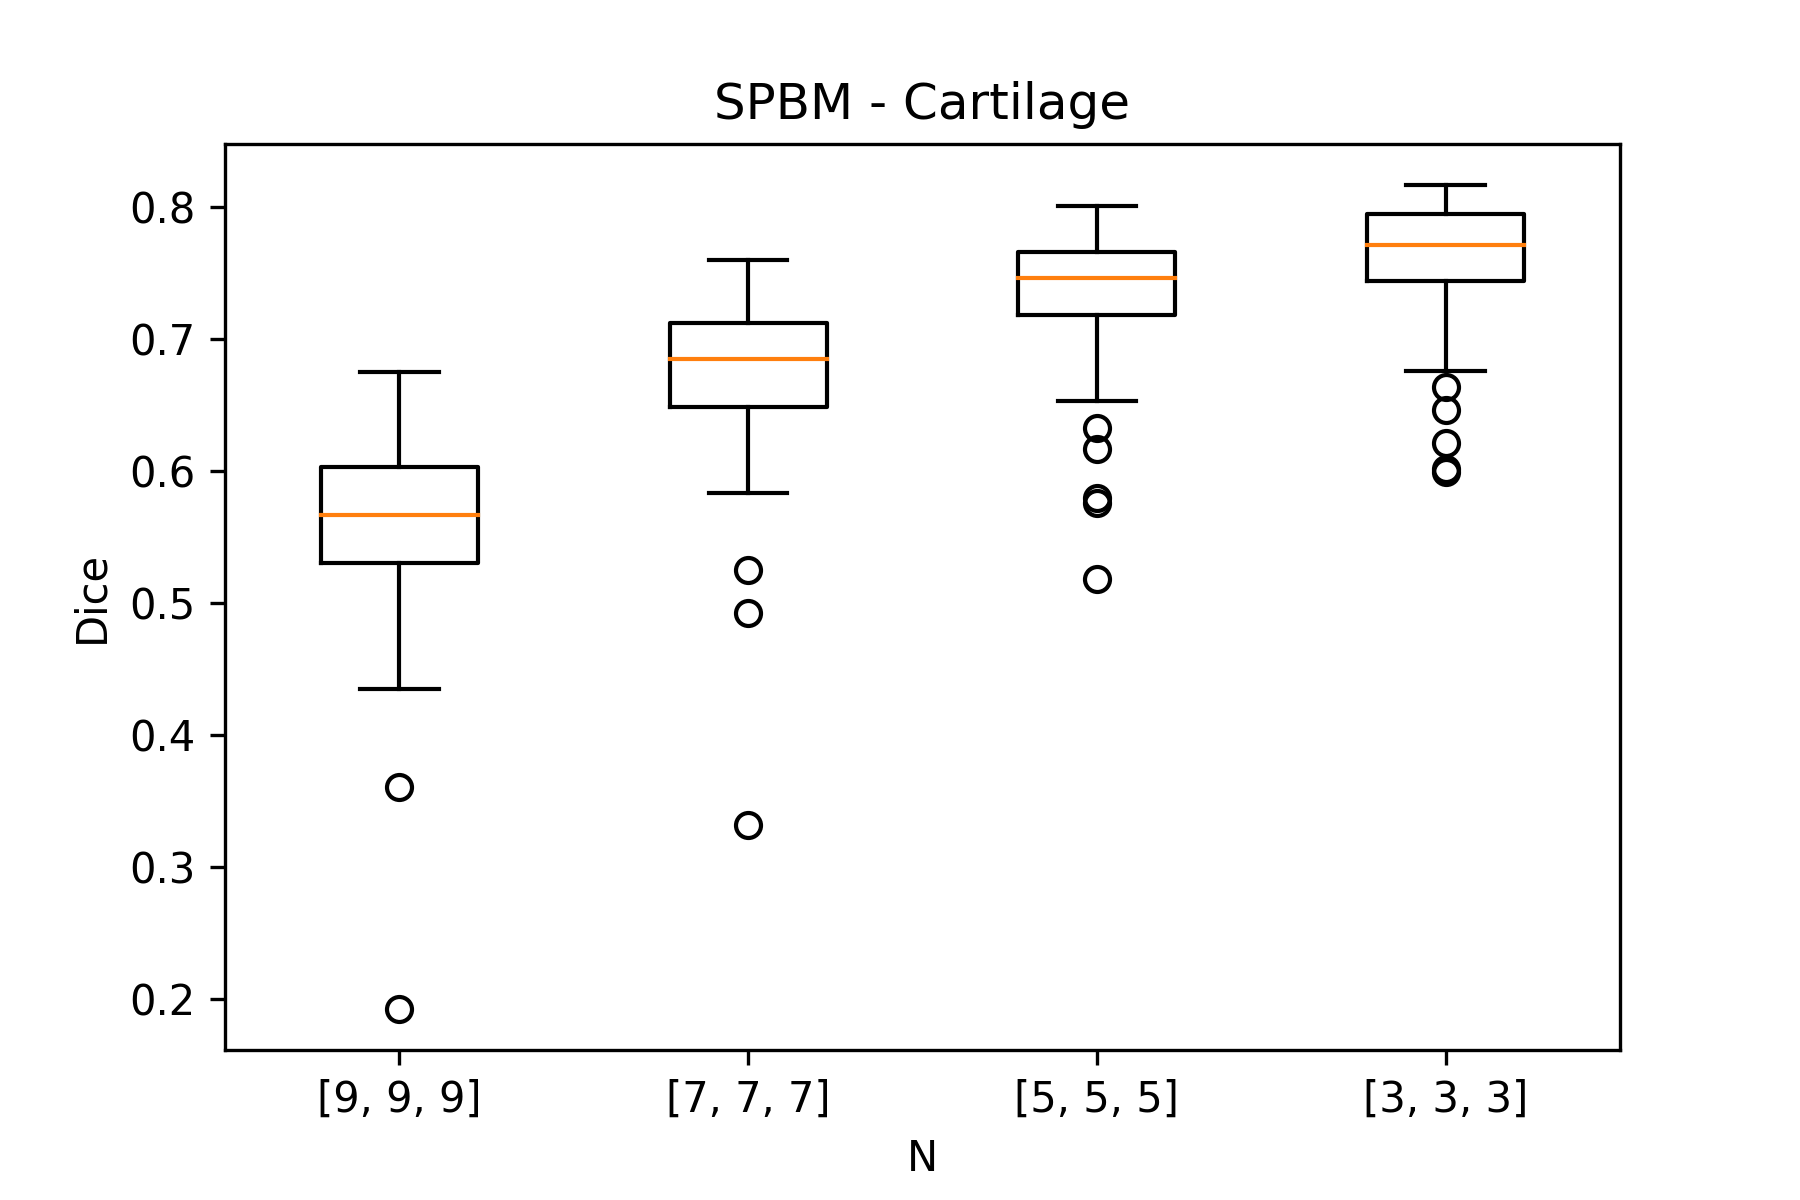
\includegraphics[width=0.85\linewidth]{SPBM_N_Cartilage_plot.png}
    \caption{Μεταβολή του τμήματος αναζήτησης της αραιής μεθόδου βασισμένης σε
             τμήματα για την ετικέτα των χόνδρων.}
    \label{fig:SPBM:N:3}
\end{figure}

\paragraphLine{Ταξινόμηση αραιής αναπαράστασης}

Τα πειράματα για την επιλογή του τμήματος αναζήτησης έγιναν με τις σταθερές
παραμέτρους που παρουσιάζονται στον \autoref{table:N:SRC}.

\begin{table}[h!]
    \centering
    \begin{tabular}{|c|c|} 
        \hline
        Παράμετρος $\lambda$ & 0.1 \\ 
        \hline
        Αριθμός ατλάντων & 4 \\ 
        \hline
        Τμήμα χαρακτηριστικών & [3,3,3] \\ 
        \hline
    \end{tabular}
    \caption{Παράμετροι που παραμένουν σταθεροί για την επιλογή του τμήματος
             αναζήτησης της μεθόδου ταξινόμησης αραιής αναπαράστασης.}
    \label{table:N:SRC}
\end{table}

Στα \autoref{fig:SRC:N:1}, \autoref{fig:SRC:N:2} και \autoref{fig:SRC:N:3}
παρουσιάζονται οι τιμές του συντελεστή ομοιότητας Dice για διάφορες τιμές του
τμήματος αναζήτησης. Παρατηρείται ότι το φαινόμενο που εμφανίζεται στην αραιή
μέθοδος βασισμένη σε τμήματα όπου, για μικρότερες τιμές του τμήματος το
αποτέλεσμα είναι καλύτερο, εμφανίζεται πιο έντονα και σε αυτή τη μέθοδο. Με τον
ίδιο συλλογισμό που ακολουθήθηκε στην προηγούμενη μέθοδο, επιλέχτηκε η τιμή
$[3,3,3]$ του τμήματος αναζήτησης.

\begin{figure}[H]
    \centering
    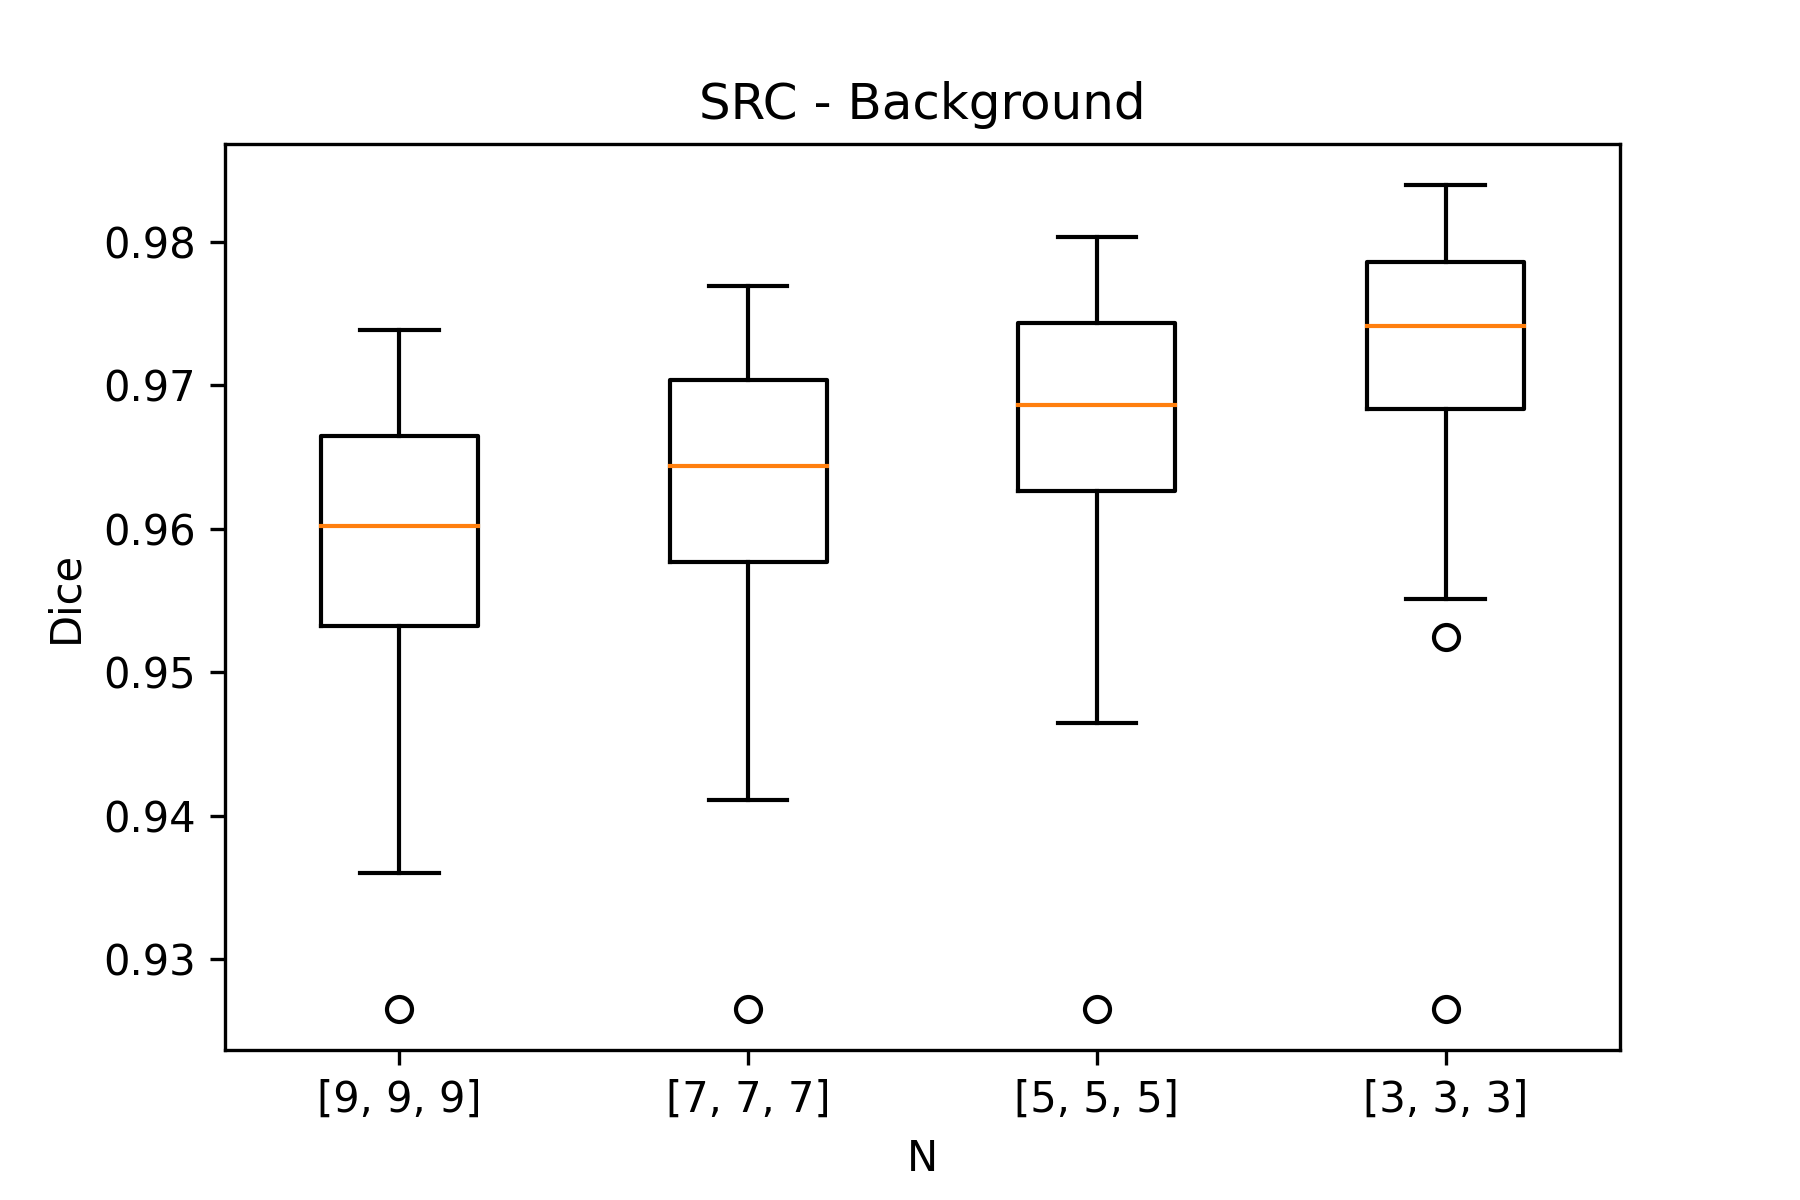
\includegraphics[width=0.85\linewidth]{SRC_N_Background_plot.png}
    \caption{Μεταβολή του τμήματος αναζήτησης της μεθόδου ταξινόμησης αραιής
             αναπαράστασης για την ετικέτα του παρασκηνίου.}
    \label{fig:SRC:N:1}
\end{figure}

\begin{figure}[H]
    \centering
    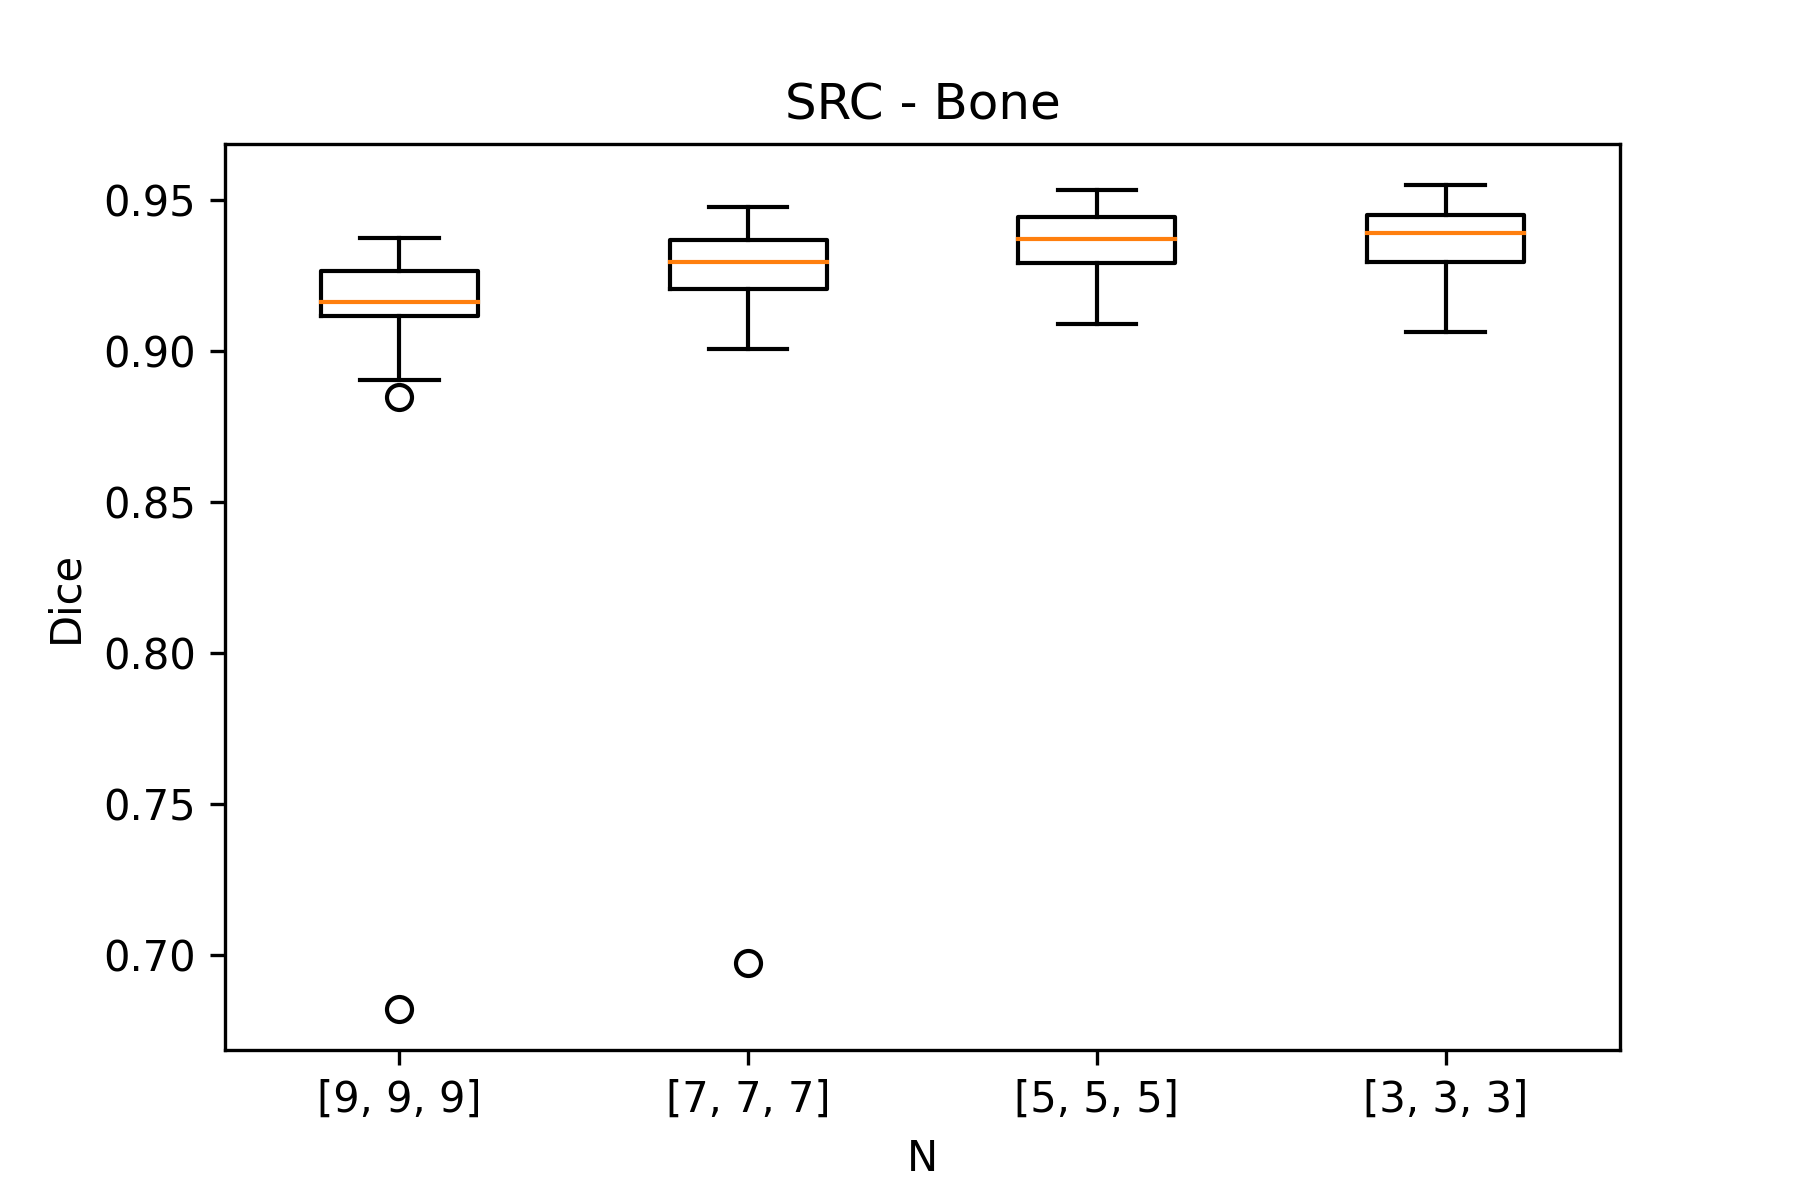
\includegraphics[width=0.85\linewidth]{SRC_N_Bone_plot.png}
    \caption{Μεταβολή του τμήματος αναζήτησης της μεθόδου ταξινόμησης αραιής
             αναπαράστασης για την ετικέτα των οστών.}
    \label{fig:SRC:N:2}
\end{figure}

\begin{figure}[H]
    \centering
    \includegraphics[width=0.85\linewidth]{SRC_N_Cartilage_plot.png}
    \caption{Μεταβολή του τμήματος αναζήτησης της μεθόδου ταξινόμησης αραιής
             αναπαράστασης για την ετικέτα των χόνδρων.}
    \label{fig:SRC:N:3}
\end{figure}

\paragraphLine{Κατάτμηση βασισμένη σε τμήματα με τη χρήση πληροφορίας από
               ειδικούς}

Τα πειράματα για την επιλογή του τμήματος αναζήτησης έγιναν με τις σταθερές
παραμέτρους που παρουσιάζονται στον \autoref{table:N:2}.

\begin{table}[h!]
    \centering
    \begin{tabular}{|c|c|} 
        \hline
        Αριθμός ατλάντων & 4 \\ 
        \hline
        Τμήμα χαρακτηριστικών & [3,3,3] \\ 
        \hline
    \end{tabular}
    \caption{Παράμετροι που παραμένουν σταθεροί για την επιλογή του τμήματος
             αναζήτησης για τη μέθοδο κατάτμησης βασισμένη σε τμήματα με τη
             χρήση πληροφορίας από ειδικούς.}
    \label{table:N:2}
\end{table}

Στα \autoref{fig:PBSEP:N:1}, \autoref{fig:PBSEP:N:2} και \autoref{fig:PBSEP:N:3}
παρουσιάζονται οι τιμές του συντελεστή ομοιότητας Dice για διάφορες τιμές του
τμήματος αναζήτησης. Παρατηρείται ότι για μεγαλύτερες τιμές του τμήματος
αναζήτησης το αποτέλεσμα είναι καλύτερο. Όσο μεγαλώνει το τμήμα αναζήτησης η
μεταβολή της απόδοσης είναι μικρότερη και για τιμή $[7,7,7]$ μηδαμινή. Για το
λόγο αυτό και υπολογιστικής ταχύτητας επιλέχτηκε η τιμή $[7,7,7]$ του τμήματος
αναζήτησης.

\begin{figure}[H]
    \centering
    \includegraphics[width=0.85\linewidth]{PBSEP_N_Background_plot.png}
    \caption{Μεταβολή του τμήματος αναζήτησης της μεθόδου κατάτμησης βασισμένη
             σε τμήματα με τη χρήση πληροφορίας από ειδικούς για την ετικέτα του
             παρασκηνίου.}
    \label{fig:PBSEP:N:1}
\end{figure}

\begin{figure}[H]
    \centering
    \includegraphics[width=0.85\linewidth]{PBSEP_N_Bone_plot.png}
    \caption{Μεταβολή του τμήματος αναζήτησης της μεθόδου κατάτμησης βασισμένη
             σε τμήματα με τη χρήση πληροφορίας από ειδικούς για την ετικέτα των
             οστών.}
    \label{fig:PBSEP:N:2}
\end{figure}

\begin{figure}[H]
    \centering
    \includegraphics[width=0.85\linewidth]{PBSEP_N_Cartilage_plot.png}
    \caption{Μεταβολή του τμήματος αναζήτησης της μεθόδου κατάτμησης βασισμένη
             σε τμήματα με τη χρήση πληροφορίας από ειδικούς για την ετικέτα των
             χόνδρων.}
    \label{fig:PBSEP:N:3}
\end{figure}


\subsubsection{Τμήμα χαρακτηριστικών}

\paragraphLine{Αραιή μέθοδος βασισμένη σε τμήματα}

Τα πειράματα για την επιλογή του τμήματος χαρακτηριστικών έγιναν με τις σταθερές
παραμέτρους που παρουσιάζονται στον \autoref{table:P:1}.

\begin{table}[h!]
    \centering
    \begin{tabular}{|c|c|} 
        \hline
        Παράμετρος $\lambda$ & 0.01 \\ 
        \hline
        Αριθμός ατλάντων & 4 \\ 
        \hline
        Τμήμα αναζήτησης & [3,3,3] \\ 
        \hline
    \end{tabular}
    \caption{Παράμετροι που παραμένουν σταθεροί για την επιλογή του τμήματος
             χαρακτηριστικών της αραιής μεθόδου βασισμένης σε τμήματα.}
    \label{table:P:1}
\end{table}

Στα \autoref{fig:SPBM:P:1}, \autoref{fig:SPBM:P:2} και \autoref{fig:SPBM:P:3}
παρουσιάζονται οι τιμές του συντελεστή ομοιότητας Dice για διάφορες τιμές του
τμήματος χαρακτηριστικών. Παρατηρείται, κυρίως στο \autoref{fig:SPBM:P:3}, ότι
για μεγαλύτερες τιμές του τμήματος χαρακτηριστικών το αποτέλεσμα είναι καλύτερο.
Για το λόγο αυτό επιλέχτηκε η τιμή $[9,9,9]$ του τμήματος χαρακτηριστικών.

\begin{figure}[H]
    \centering
    \includegraphics[width=0.85\linewidth]{SPBM_P_Background_plot.png}
    \caption{Μεταβολή του τμήματος χαρακτηριστικών της αραιής μεθόδου βασισμένης
             σε τμήματα για την ετικέτα του παρασκηνίου.}
    \label{fig:SPBM:P:1}
\end{figure}

\begin{figure}[H]
    \centering
    \includegraphics[width=0.85\linewidth]{SPBM_P_Bone_plot.png}
    \caption{Μεταβολή του τμήματος χαρακτηριστικών της αραιής μεθόδου βασισμένης
             σε τμήματα για την ετικέτα των οστών.}
    \label{fig:SPBM:P:2}
\end{figure}

\begin{figure}[H]
    \centering
    \includegraphics[width=0.85\linewidth]{SPBM_P_Cartilage_plot.png}
    \caption{Μεταβολή του τμήματος χαρακτηριστικών της αραιής μεθόδου βασισμένης
             σε τμήματα για την ετικέτα των χόνδρων.}
    \label{fig:SPBM:P:3}
\end{figure}

\paragraphLine{Ταξινόμηση αραιής αναπαράστασης}

Τα πειράματα για την επιλογή του τμήματος χαρακτηριστικών έγιναν με τις σταθερές
παραμέτρους που παρουσιάζονται στον \autoref{table:P:SRC}.

\begin{table}[h!]
    \centering
    \begin{tabular}{|c|c|} 
        \hline
        Παράμετρος $\lambda$ & 0.1 \\ 
        \hline
        Αριθμός ατλάντων & 4 \\ 
        \hline
        Τμήμα αναζήτησης & [3,3,3] \\ 
        \hline
    \end{tabular}
    \caption{Παράμετροι που παραμένουν σταθεροί για την επιλογή του τμήματος
             χαρακτηριστικών της μεθόδου ταξινόμησης αραιής αναπαράστασης.}
    \label{table:P:SRC}
\end{table}

Στα \autoref{fig:SRC:P:1}, \autoref{fig:SRC:P:2} και \autoref{fig:SRC:P:3}
παρουσιάζονται οι τιμές του συντελεστή ομοιότητας Dice για διάφορες τιμές του
τμήματος χαρακτηριστικών. Παρατηρείται, κυρίως στο \autoref{fig:SRC:P:3}, ότι
για μεγαλύτερες τιμές του τμήματος χαρακτηριστικών το αποτέλεσμα είναι καλύτερο.
Για το λόγο αυτό επιλέχτηκε η τιμή $[9,9,9]$ του τμήματος χαρακτηριστικών.

\begin{figure}[H]
    \centering
    \includegraphics[width=0.85\linewidth]{SRC_P_Background_plot.png}
    \caption{Μεταβολή του τμήματος χαρακτηριστικών της μεθόδου ταξινόμησης
             αραιής αναπαράστασης για την ετικέτα του παρασκηνίου.}
    \label{fig:SRC:P:1}
\end{figure}

\begin{figure}[H]
    \centering
    \includegraphics[width=0.85\linewidth]{SRC_P_Bone_plot.png}
    \caption{Μεταβολή του τμήματος χαρακτηριστικών της μεθόδου ταξινόμησης
             αραιής αναπαράστασης για την ετικέτα των οστών.}
    \label{fig:SRC:P:2}
\end{figure}

\begin{figure}[H]
    \centering
    \includegraphics[width=0.85\linewidth]{SRC_P_Cartilage_plot.png}
    \caption{Μεταβολή του τμήματος χαρακτηριστικών της μεθόδου ταξινόμησης
             αραιής αναπαράστασης για την ετικέτα των χόνδρων.}
    \label{fig:SRC:P:3}
\end{figure}

\paragraphLine{Κατάτμηση βασισμένη σε τμήματα με τη χρήση πληροφορίας από
               ειδικούς}

Τα πειράματα για την επιλογή του τμήματος χαρακτηριστικών έγιναν με τις σταθερές
παραμέτρους που παρουσιάζονται στον \autoref{table:P:2}.

\begin{table}[h!]
    \centering
    \begin{tabular}{|c|c|} 
        \hline
        Αριθμός ατλάντων & 4 \\ 
        \hline
        Τμήμα χαρακτηριστικών & [7,7,7] \\ 
        \hline
    \end{tabular}
    \caption{Παράμετροι που παραμένουν σταθεροί για την επιλογή του τμήματος
             χαρακτηριστικών για τη μέθοδο κατάτμησης βασισμένη σε τμήματα με τη
             χρήση πληροφορίας από ειδικούς.}
    \label{table:P:2}
\end{table}

Στα \autoref{fig:PBSEP:P:1}, \autoref{fig:PBSEP:P:2} και \autoref{fig:PBSEP:P:3}
παρουσιάζονται οι τιμές του συντελεστή ομοιότητας Dice για διάφορες τιμές του
τμήματος χαρακτηριστικών. Παρατηρείται ότι για όλες τις τιμές του τμήματος
χαρακτηριστικών η απόδοση είναι παρόμοια. Για το λόγο αυτό και υπολογιστικής
ταχύτητας επιλέχτηκε η τιμή $[3,3,3]$ του τμήματος αναζήτησης.

\begin{figure}[H]
    \centering
    \includegraphics[width=0.85\linewidth]{PBSEP_P_Background_plot.png}
    \caption{Μεταβολή του τμήματος χαρακτηριστικών της μεθόδου κατάτμησης
             βασισμένη σε τμήματα με τη χρήση πληροφορίας από ειδικούς για την
             ετικέτα του παρασκηνίου.}
    \label{fig:PBSEP:P:1}
\end{figure}

\begin{figure}[H]
    \centering
    \includegraphics[width=0.85\linewidth]{PBSEP_P_Bone_plot.png}
    \caption{Μεταβολή του τμήματος χαρακτηριστικών της μεθόδου κατάτμησης
             βασισμένη σε τμήματα με τη χρήση πληροφορίας από ειδικούς για την
             ετικέτα των οστών.}
    \label{fig:PBSEP:P:2}
\end{figure}

\begin{figure}[H]
    \centering
    \includegraphics[width=0.85\linewidth]{PBSEP_P_Cartilage_plot.png}
    \caption{Μεταβολή του τμήματος χαρακτηριστικών της μεθόδου κατάτμησης
             βασισμένη σε τμήματα με τη χρήση πληροφορίας από ειδικούς για την
             ετικέτα των χόνδρων.}
    \label{fig:PBSEP:P:3}
\end{figure}

\subsubsection{Αριθμός ατλάντων}

\paragraphLine{Αραιή μέθοδος βασισμένη σε τμήματα}

Τα πειράματα για την επιλογή του αριθμού των ατλάντων έγιναν με τις σταθερές
παραμέτρους που παρουσιάζονται στον \autoref{table:atlases:1}.

\begin{table}[h!]
    \centering
    \begin{tabular}{|c|c|} 
        \hline
        Παράμετρος $\lambda$ & 0.01 \\ 
        \hline
        Τμήμα αναζήτησης & [3,3,3] \\ 
        \hline
        Τμήμα χαρακτηριστικών & [9,9,9] \\ 
        \hline
    \end{tabular}
    \caption{Παράμετροι που παραμένουν σταθεροί για την επιλογή του αριθμού των
             ατλάντων της αραιής μεθόδου βασισμένης σε τμήματα.}
    \label{table:atlases:1}
\end{table}

Στα \autoref{fig:SPBM:atlases:1}, \autoref{fig:SPBM:atlases:2} και
\autoref{fig:SPBM:atlases:3} παρουσιάζονται οι τιμές του συντελεστή ομοιότητας
Dice για διάφορες τιμές του αριθμού των ατλάντων. Παρατηρείται ότι για
μεγαλύτερες τιμές του αριθμού των ατλάντων το αποτέλεσμα είναι καλύτερο. Επίσης,
για $9$ άτλαντες υπάρχει κορεσμός του αποτελέσματος. Για το λόγο αυτό επιλέχτηκε
η τιμή $9$ του αριθμού των ατλάντων.

\begin{figure}[H]
    \centering
    \includegraphics[width=0.85\linewidth]{SPBM_Number_of_atlases_Background_plot.png}
    \caption{Μεταβολή του αριθμού των ατλάντων της αραιής μεθόδου βασισμένης σε
             τμήματα για την ετικέτα του παρασκηνίου.}
    \label{fig:SPBM:atlases:1}
\end{figure}

\begin{figure}[H]
    \centering
    \includegraphics[width=0.85\linewidth]{SPBM_Number_of_atlases_Bone_plot.png}
    \caption{Μεταβολή του αριθμού των ατλάντων της αραιής μεθόδου βασισμένης σε
             τμήματα για την ετικέτα των οστών.}
    \label{fig:SPBM:atlases:2}
\end{figure}

\begin{figure}[H]
    \centering
    \includegraphics[width=0.85\linewidth]{SPBM_Number_of_atlases_Cartilage_plot.png}
    \caption{Μεταβολή του αριθμού των ατλάντων της αραιής μεθόδου βασισμένης σε
             τμήματα για την ετικέτα των χόνδρων.}
    \label{fig:SPBM:atlases:3}
\end{figure}

\paragraphLine{Ταξινόμηση αραιής αναπαράστασης}

Τα πειράματα για την επιλογή του του αριθμού των ατλάντων έγιναν με τις σταθερές
παραμέτρους που παρουσιάζονται στον \autoref{table:atlases:SRC}.

\begin{table}[h!]
    \centering
    \begin{tabular}{|c|c|} 
        \hline
        Παράμετρος $\lambda$ & 0.1 \\ 
        \hline
        Τμήμα αναζήτησης & [3,3,3] \\ 
        \hline
        Τμήμα χαρακτηριστικών & [9,9,9] \\ 
        \hline
    \end{tabular}
    \caption{Παράμετροι που παραμένουν σταθεροί για την επιλογή του αριθμού των
             ατλάντων της μεθόδου ταξινόμησης αραιής αναπαράστασης.}
    \label{table:atlases:SRC}
\end{table}

Στα \autoref{fig:SRC:atlases:1}, \autoref{fig:SRC:atlases:2} και
\autoref{fig:SRC:atlases:3} παρουσιάζονται οι τιμές του συντελεστή ομοιότητας
Dice για διάφορες τιμές του αριθμού των ατλάντων. Παρατηρείται ότι για μεγάλες
τιμές του αριθμού των ατλάντων το αποτέλεσμα είναι καλύτερο. Επίσης, όπως και
στην αραιή μέθοδο βασισμένη σε τμήματα, για $9$ άτλαντες υπάρχει κορεσμός του
αποτελέσματος. Για το λόγο αυτό επιλέχτηκε η τιμή $9$ του αριθμού των ατλάντων.

\begin{figure}[H]
    \centering
    \includegraphics[width=0.85\linewidth]{SRC_Number_of_atlases_Background_plot.png}
    \caption{Μεταβολή του αριθμού των ατλάντων της μεθόδου ταξινόμησης αραιής
             αναπαράστασης για την ετικέτα του παρασκηνίου.}
    \label{fig:SRC:atlases:1}
\end{figure}

\begin{figure}[H]
    \centering
    \includegraphics[width=0.85\linewidth]{SRC_Number_of_atlases_Bone_plot.png}
    \caption{Μεταβολή του αριθμού των ατλάντων της μεθόδου ταξινόμησης αραιής
             αναπαράστασης για την ετικέτα των οστών.}
    \label{fig:SRC:atlases:2}
\end{figure}

\begin{figure}[H]
    \centering
    \includegraphics[width=0.85\linewidth]{SRC_Number_of_atlases_Cartilage_plot.png}
    \caption{Μεταβολή του αριθμού των ατλάντων της μεθόδου ταξινόμησης αραιής
             αναπαράστασης για την ετικέτα των χόνδρων.}
    \label{fig:SRC:atlases:3}
\end{figure}

\paragraphLine{Κατάτμηση βασισμένη σε τμήματα με τη χρήση πληροφορίας από
               ειδικούς}

Τα πειράματα για την επιλογή του αριθμού των ατλάντων έγιναν με τις σταθερές
παραμέτρους που παρουσιάζονται στον \autoref{table:atlases:2}.

\begin{table}[h!]
    \centering
    \begin{tabular}{|c|c|} 
        \hline
        Τμήμα αναζήτησης & [7,7,7] \\ 
        \hline
        Τμήμα χαρακτηριστικών & [3,3,3] \\ 
        \hline
    \end{tabular}
    \caption{Παράμετροι που παραμένουν σταθεροί για την επιλογή του αριθμού των
             ατλάντων για τη μέθοδο κατάτμησης βασισμένη σε τμήματα με τη χρήση
             πληροφορία από ειδικούς.}
    \label{table:atlases:2}
\end{table}

Στα \autoref{fig:PBSEP:atlases:1}, \autoref{fig:PBSEP:atlases:2} και
\autoref{fig:PBSEP:atlases:3} παρουσιάζονται οι τιμές του συντελεστή ομοιότητας
Dice για διάφορες τιμές του αριθμού των ατλάντων. Παρατηρείται ότι για
μεγαλύτερες τιμές του αριθμού των ατλάντων το αποτέλεσμα είναι καλύτερο. Επίσης,
όπως και στις προηγούμενες μεθόδους, υπάρχει κορεσμός του αποτελέσματος για $9$
άτλαντες. Για το λόγο αυτό επιλέγεται η τιμή $9$ για τον αριθμό των ατλάντων.

\begin{figure}[H]
    \centering
    \includegraphics[width=0.85\linewidth]{PBSEP_Number_of_atlases_Background_plot.png}
    \caption{Μεταβολή του αριθμού των ατλάντων της μεθόδου κατάτμησης βασισμένη
             σε τμήματα με τη χρήση πληροφορίας από ειδικούς για την ετικέτα του
             παρασκηνίου.}
    \label{fig:PBSEP:atlases:1}
\end{figure}

\begin{figure}[H]
    \centering
    \includegraphics[width=0.85\linewidth]{PBSEP_Number_of_atlases_Bone_plot.png}
    \caption{Μεταβολή του αριθμού των ατλάντων της μεθόδου κατάτμησης βασισμένη
             σε τμήματα με τη χρήση πληροφορίας από ειδικούς για την ετικέτα των
             οστών.}
    \label{fig:PBSEP:atlases:2}
\end{figure}

\begin{figure}[H]
    \centering
    \includegraphics[width=0.85\linewidth]{PBSEP_Number_of_atlases_Cartilage_plot.png}
    \caption{Μεταβολή του αριθμού των ατλάντων της μεθόδου κατάτμησης βασισμένη
             σε τμήματα με τη χρήση πληροφορίας από ειδικούς για την ετικέτα των
             χόνδρων.}
    \label{fig:PBSEP:atlases:3}
\end{figure}


\subsection{Σύγκριση μεθόδων}

\subsubsection{Σύγκριση απόδοσης}

Στα \autoref{fig:dice_final:1}, \autoref{fig:dice_final:2} και
\autoref{fig:dice_final:3} παρουσιάζονται οι τιμές του συντελεστή ομοιότητας
Dice για όλες τις μεθόδους. Παρατηρείται, ιδίως στο \autoref{fig:dice_final:3},
ότι η μέθοδος κατάτμησης βασισμένη σε τμήματα με τη χρήση πληροφορίας από
ειδικούς έχει το καλύτερο αποτέλεσμα. Ακόμα, παρατηρείται ότι η αραιή μέθοδος
βασισμένη σε τμήματα έχει καλύτερο αποτέλεσμα στην ετικέτα των χόνδρων από την
μέθοδο ταξινόμησης αραιής αναπαράστασης, ενώ το αντίθετο συμβαίνει στην ετικέτα
των οστών σε πιο μικρό βαθμό. Το αποτέλεσμα για την ετικέτα του παρασκηνίου
είναι παρόμοιο για όλες τις μεθόδους. 

Ακόμα στα παραπάνω σχήματα παρουσιάζονται πειράματα όπου το αποτέλεσμα τους
είναι πολύ χειρότερο σε σχέση με τα υπόλοιπα αποτελέσματα. Αυτό μπορεί να
οφείλεται είτε σε απεικονίσεις που διαφέρουν σε σχέση με τους άτλαντες, είτε στη
καταχώρηση και επιλογή των ατλάντων.

Στο \autoref{table:final_reuslts:1} παρουσιάζονται οι τιμές της μέσης τιμής και
της διαμέσου για όλες τις ετικέτες και μεθόδους. Ο πίνακας αυτός επιβεβαιώνει τα
συμπεράσματα της προηγούμενης παραγράφου.

Τέλος, στα \autoref{fig:final_dice_SPBM}, \autoref{fig:final_dice_SPBM}
και \autoref{fig:final_dice_SPBM} παρουσιάζεται το χειρότερο, μέσο και καλύτερο
αποτέλεσμα βάση της ετικέτας των χόνδρων για κάθε μέθοδο.


\begin{figure}[H]
    \centering
    \includegraphics[width=0.85\linewidth]{Dice_final_Background_plot.png}
    \caption{Για όλες τις μεθόδους η τιμή του συντελεστή ομοιότητας Dice για την
             ετικέτα του παρασκηνίου.}
    \label{fig:dice_final:1}
\end{figure}

\begin{figure}[H]
    \centering
    \includegraphics[width=0.85\linewidth]{Dice_final_Bone_plot.png}
    \caption{Για όλες τις μεθόδους η τιμή του συντελεστή ομοιότητας Dice για την
             ετικέτα των οστών.}
    \label{fig:dice_final:2}
\end{figure}

\begin{figure}[H]
    \centering
    \includegraphics[width=0.85\linewidth]{Dice_final_Cartilage_plot.png}
    \caption{Για όλες τις μεθόδους η τιμή του συντελεστή ομοιότητας Dice για την
             ετικέτα των χόνδρων.}
    \label{fig:dice_final:3}
\end{figure}

\begin{table}[h!]
    \centering
    \begin{tabular}{|c|c||c|c|} 
        \hline
        Μέθοδος & Ετικέτα & Μέσος όρος & Διάμεσος \\ 
        \hline
        \hline
        \multirow{3}{4em}{SPBM} & Παρασκήνιο & 0.9914 & 0.9926 \\ 
        & Οστά & 0.9521 & 0.9556 \\ 
        & Χόνδροι & 0.8209 & 0.8352 \\ 
        \hline
        \multirow{3}{4em}{SRC} & Παρασκήνιο & 0.9914 & 0.9926 \\ 
        & Οστά & 0.9528 & 0.9585 \\ 
        & Χόνδροι & 0.8056 & 0.8187 \\ 
        \hline
        \multirow{3}{4em}{PBSEP} & Παρασκήνιο & 0.9916 & 0.9933 \\ 
        & Οστά & 0.956 & 0.9624 \\ 
        & Χόνδροι & 0.8281 & 0.8451 \\ 
        \hline
    \end{tabular}
    \caption{Μέσος όρος και διάμεσος του συντελεστή ομοιότητας Dice για όλες
             τις μεθόδους και ετικέτες.}
    \label{table:final_reuslts:1}
\end{table}

\begin{figure}[H]
    \centering

    \begin{subfigure}[b]{0.32\linewidth}
    \includegraphics[width=\linewidth]{final_SPBM_worst.png}
    \caption{Dice = 0.6614}
    \end{subfigure}
    \begin{subfigure}[b]{0.32\linewidth}
    \includegraphics[width=\linewidth]{final_SPBM_median.png}
    \caption{Dice = 0.8352}
    \end{subfigure}
    \begin{subfigure}[b]{0.32\linewidth}
    \includegraphics[width=\linewidth]{final_SPBM_best.png}
    \caption{Dice = 0.8604}
    \end{subfigure}

    \caption{Το χειρότερο (αριστερά), μέσο (μέση) και καλύτερο (δεξιά)
             αποτέλεσμα, βάση της ετικέτας των χόνδρων, για την αραιή μέθοδο
             βασισμένη σε τμήματα.}
    \label{fig:final_dice_SPBM}
\end{figure}

\begin{figure}[H]
    \centering

    \begin{subfigure}[b]{0.32\linewidth}
    \includegraphics[width=\linewidth]{final_SRC_worst.png}
    \caption{Dice = 0.662}
    \end{subfigure}
    \begin{subfigure}[b]{0.32\linewidth}
    \includegraphics[width=\linewidth]{final_SRC_median.png}
    \caption{Dice = 0.8187}
    \end{subfigure}
    \begin{subfigure}[b]{0.32\linewidth}
    \includegraphics[width=\linewidth]{final_SRC_best.png}
    \caption{Dice = 0.8578}
    \end{subfigure}

    \caption{Το χειρότερο (αριστερά), μέσο (μέση) και καλύτερο (δεξιά)
             αποτέλεσμα, βάση της ετικέτας των χόνδρων, για τη μέθοδο
             ταξινόμησης αραιής αναπαράστασης.}
    \label{fig:final_dice_SRC}
\end{figure}

\begin{figure}[H]
    \centering

    \begin{subfigure}[b]{0.32\linewidth}
    \includegraphics[width=\linewidth]{final_SPEP_worst.png}
    \caption{Dice = 0.6614}
    \end{subfigure}
    \begin{subfigure}[b]{0.32\linewidth}
    \includegraphics[width=\linewidth]{final_SPEP_median.png}
    \caption{Dice = 0.8352}
    \end{subfigure}
    \begin{subfigure}[b]{0.32\linewidth}
    \includegraphics[width=\linewidth]{final_SPEP_best.png}
    \caption{Dice = 0.8604}
    \end{subfigure}

    \caption{Το χειρότερο (αριστερά), μέσο (μέση) και καλύτερο (δεξιά)
             αποτέλεσμα, βάση της ετικέτας των χόνδρων, για τη μέθοδο κατάτμησης
             βασισμένης σε τμήματα με τη χρήση πληροφορίας από ειδικούς.}
    \label{fig:final_dice_SPEP}
\end{figure}

\subsubsection{Σύγκριση χρόνου εκτέλεσης}

Τα πειράματα έτρεξαν σε υπολογιστή με επεξεργαστή τον \emph{Intel(R) Core(TM)
i9-7940X CPU @ 3.10GHz} και \emph{126GB} μνήμη. Κάθε πείραμα έτρεχε σε ένα νήμα
(thread) και για τον υπολογισμό των χρόνων έτρεχαν παράλληλα \emph{14} νήματα
(ένα για κάθε πείραμα).

Στο \autoref{fig:registration_time:1} παρουσιάζεται ο χρόνος εκτέλεσης για κάθε
μέθοδο της προεπεξεργασίας (μαζί με το διάβασμα των αρχείων) και της καταχώρησης
όλων των ατλάντων (45 άτλαντες). Οι χρόνοι είναι παρόμοιοι αλλά υπάρχει μία
μικρή διακύμανση. Επειδή ο κώδικας που υλοποιεί αυτό το κομμάτι για κάθε μέθοδο
είναι ο ίδιος το αποτέλεσμα είναι αναμενόμενο.

Στο \autoref{fig:segmentation_time:1} παρουσιάζεται αποκλειστικά ο χρόνος
εκτέλεσης της κατάτμησης (χωρίς ανάγνωση δεδομένων, προεπεξεργασία, καταχώρηση,
αξιολόγηση και αποθήκευση του αποτελέσματος). Αρχικά, παρατηρείται ότι η μέθοδος
κατάτμησης βασισμένη σε τμήματα με τη χρήση πληροφορίας από ειδικούς είναι η πιο
γρήγορη. Αυτό είναι αναμενόμενο αφού είναι η πιο απλή μέθοδος αφού δεν
περιλαμβάνει την επίλυση του ελάχιστα απόλυτου τελεστή συρρίκνωσης και επιλογής
όπως οι άλλες μέθοδοι. Ακόμα, παρατηρείται ότι η αραιή μέθοδος βασισμένη σε
τμήματα είναι πιο γρήγορη από τη μέθοδο ταξινόμησης αραιής αναπαράστασης. Αυτό
οφείλεται στη μοναδική διαφορά των μεθόδων δηλαδή, στον υπολογισμό της ετικέτας
έχοντας τους συντελεστές ανοικοδόμησης.

Στο \autoref{fig:total_time:1} παρουσιάζεται ο χρόνος εκτέλεσης ολόκληρης της
διαδικασίας της κατάτμησης για όλες τις μεθόδους. Επειδή η μόνη διαφορά στις
μεθόδους είναι η διαδικασία της καταχώρησης, το αποτέλεσμα είναι αναμενόμενα
σύμφωνα με τα αποτελέσματα της προηγούμενης παραγράφου.


\begin{figure}[H]
    \centering
    \includegraphics[width=0.85\linewidth]{Registration_time_plot.png}
    \caption{Ο χρόνος εκτέλεσης της προεπεξεργασίας και της καταχώρησης των
             ατλάντων για όλες τις μεθόδους.}
    \label{fig:registration_time:1}
\end{figure}

\begin{figure}[H]
    \centering
    \includegraphics[width=0.85\linewidth]{Segmentation_time_plot.png}
    \caption{Ο χρόνος εκτέλεσης της κατάτμησης (χωρίς την προεπεξεργασία, την
             καταχώρηση, αξιολόγηση και αποθήκευση των αποτελεσμάτων) για όλες
             τις μεθόδους.} 
    \label{fig:segmentation_time:1}
\end{figure}

\begin{figure}[H]
    \centering
    \includegraphics[width=0.85\linewidth]{Total_time_plot.png}
    \caption{Ο συνολικός χρόνος εκτέλεσης ολόκληρης της διαδικασίας της
             κατάτμησης για όλες τις μεθόδους.} 
    \label{fig:total_time:1}
\end{figure}


\section{Συμπεράσματα και μελλοντική εργασία}

\subsection{Συμπεράσματα} \label{conclusions}

Στο πλαίσιο της παρούσας διπλωματικής εργασίας, μελετήθηκε η κατάτμηση των
αρθρικών χόνδρων και οστών απεικονίσεων μαγνητικής τομογραφίας στη περιοχή των
γονάτων με μεθόδους μηχανικής μάθησης. Εφαρμόστηκαν τρεις διαφορετικές μέθοδοι
\cite{Zhang:1} \cite{Tong:1} \cite{Coupe:1} που είχαν εφαρμοστεί στη περιοχή του
εγκεφάλου. Και για τις τρεις μεθόδους χρησιμοποιήθηκε η ίδια μέθοδος
προεπεξεργασίας και καταχώρησης.

Τα αποτελέσματα και των τριών μεθόδων ήταν ικανοποιητικά και εξαρτιόντουσαν
κυρίως από την πολυπλοκότητα της ετικέτας (π.χ. τα αποτελέσματα για τα οστά ήταν
πολύ καλύτερα σε σχέση με τα αποτελέσματα των χόνδρων σε όλες τις μεθόδους).
Επίσης και στις τρεις μεθόδους υπήρχαν πειράματα που είχαν μικρές ακραίες τιμές
(αρκετά κακό αποτέλεσμα σε σχέση με τα υπόλοιπα). Αυτό πιθανότατα οφείλεται στην
είτε στην επιλογή των ατλάντων, είτε στην καταχώρηση.

\subsection{Μελλοντική εργασία}

Στη παρούσα διπλωματική εργασία μελετήθηκε μόνο η κατάτμηση των αρθρικών χόνδρων
και οστών. Για το λόγο αυτό θα μπορούσαν να μελετηθούν περισσότερες ανατομικές
δομές στη περιοχή των γονάτων όπως ο μηνίσκος και οι σύνδεσμοι. Επίσης, η
κατηγορίες που χρησιμοποιήθηκαν θα μπορούσαν να χωριστούν σε περισσότερες
υποκατηγορίες (π.χ. να χωριστεί η κατηγορία του χόνδρου σε χόνδρου του μηρού και
της κνήμης) ώστε να υπάρχει μεγαλύτερη ακρίβεια.

Θα μπορούσε να μελετηθεί περαιτέρω η διαδικασία της καταχώρησης και της επιλογή
των ατλάντων ώστε να μειωθεί το φαινόμενο που αναφέρθηκε στο \ref{conclusions}.
Επίσης, θα μπορούσε να μελετηθεί περαιτέρω η προεπεξεργασία των δεδομένων
επειδή, δεν δόθηκε ιδιαίτερη σημασία στην παρούσα διπλωματική εργασία, ώστε να
βελτιωθεί το αποτέλεσμα.

\newpage

\addcontentsline{toc}{section}{Βιβλιογραφία}
\printbibliography[title=Βιβλιογραφία]


\end{document}
